%%%%%%%%%%%%%%%%%%%%%%%%%%%%%%%%%%%%%%%%%
%  Telemac Documentation
%  Example of the TelemacDoc class
%
%%%%%%%%%%%%%%%%%%%%%%%%%%%%%%%%%%%%%%%%%

%----------------------------------------------------------------------------------------
%	PACKAGES AND OTHER DOCUMENT CONFIGURATIONS
%----------------------------------------------------------------------------------------
\documentclass[Telemac3D]{../../data/TelemacDoc} % Default font size and left-justified equations
%\documentclass[Telemac2D,french]{TelemacDoc} % Default font size and left-justified equations in french

\begin{document}

\let\cleardoublepage\clearpage

%----------------------------------------------------------------------------------------
%	TITLE PAGE
%----------------------------------------------------------------------------------------
\title{Telemac3d}
\subtitle{User Manual}
\version{\telmaversion}
\date{\today}
\maketitle
\clearpage


%----------------------------------------------------------------------------------------
%	COPYRIGHT PAGE
%----------------------------------------------------------------------------------------

\newpage

\thispagestyle{empty}

\TelemacCopyright{}


%----------------------------------------------------------------------------------------
%	TABLE OF CONTENTS
%----------------------------------------------------------------------------------------


\pagestyle{empty} % No headers

\tableofcontents% Print the table of contents itself

%\cleardoublepage % Forces the first chapter to start on an odd page so it's on the right

\pagestyle{fancy} % Print headers again

%----------------------------------------------------------------------------------------
%	CHAPTER 1: Introduction
%----------------------------------------------------------------------------------------

\chapter{Introduction}

The \telemac{3D} code solves such three-dimensional equations as the free
surface flow equations (with or without the hydrostatic pressure hypothesis)
and the transport-diffusion equations of intrinsic quantities (temperature,
salinity, concentration). Its main results, at each point in the resolution
mesh in 3D, are the velocity in all three directions and the concentrations of
transported quantities. Water depth is the major result as regards the 2D
surface mesh. The \telemac{3D}'s prominent applications can be found in free
surface flow, in both seas and rivers; the software can take the following
processes into account:

\begin{itemize}
\item Influence of temperature and/or salinity on density,
\item Bottom friction,
\item Influence of the Coriolis force,
\item Influence of weather elements: air pressure, rain or evaporation and
wind,
\item Consideration of the thermal exchanges with the atmosphere,
\item Sources and sinks for fluid moment within the flow domain,
\item Simple or complex turbulence models ($k$-$\epsilon$) taking the
effects of the Archimedean force (buoyancy) into account,
\item Dry areas in the computational domain: tidal flats,
\item Current drift and diffusion of a tracer, with generation or
disappearance terms,
\item Oil spill modelling.
\end{itemize}

The code is applicable to many fields. The main ones are related to the marine
environment through the investigations of currents being induced either by
tides or density gradients, with or without the influence of such an external
force as the wind or the air pressure. It can be applied either to large extent
areas (on a sea scale) or to smaller domains (coasts and estuaries) for the
impact of sewer effluents, the study of thermal plumes or even sedimentary
transport. As regards the continental waters, the study of thermal plumes in
rivers, the hydrodynamic behaviour or natural or man-made lakes can be
mentioned as well.

\telemac{3D} is developed by the LNHE (Laboratoire National d'Hydraulique et
Environnement) of the Research and Development Division of EDF (EDF-R\&D). As
for previous releases, the 7.1 release of the code complies with the Quality
Assurance procedures of scientific and technical softwares of EDF-R\&D. It is a
process of construction and verification of the product quality in the
different phases of his life. In particular, a software following the Quality
Assurance procedures comes with a Validation Folder that describes the intended
use of the software and a set of test cases. This document allows you to judge
the performance and limitations of the software, situating the field of
application. These tests are also used in development of the software and are
checked at every new release.

\section{Position of the \telemac{3d} code within the telemac modelling system}

The \telemac{3D} software is part of the \tel modelling system developed by
the LNHE of EDF R\&D. \tel is a set of modelling tools allowing to treat
every aspects of natural free surface hydraulics: currents, waves, transport of
tracers and sedimentology.

The pre-processing and post-processing of simulations can be done either
directly within the \tel system or with different software that present an
interface of communication with the system. We can particularly mention the
following tools:

\begin{itemize}
\item The FUDAA-PREPRO software, developed from the FUDAA platform
by the CEREMA's Recherche, Informatique et Modélisation Department, covers all
the pre-processing tasks involved by the achievement of a numerical hydraulic
study, as well as a graphical post-processing tool,
\item The Blue Kenue software, developed the Hydraulic Canadian
Center, proposes a powerful mesh generation tool and a user-friendly
post-processing tool,
\item The Janet software, developed by Smile Consult GmbH, which offers among
others, a mesh generation tool,
\item The ParaView software, developed by Sandia National Laboratories, Los
Alamos National Laboratory and Kitware, which enables to visualise 3D results,
big data in particular and is open source,
\item The SALOME-HYDRO software based on the SALOME platform, developed by EDF,
CEA and OPENCASCADE which enables to handle raw data (bathymetry, maps,
pictures, LIDAR\ldots) until the mesh generation.
The post-processing tool ParaViS available in the SALOME platform is based on
the ParaView software and can visualise 1D, 2D or 3D results.
A first release of SALOME-HYDRO has been available since Spring 2016,
\item The Tecplot 360 software, developed by Tecplot which enables to visualise
2D and 3D results,
\item The QGIS software, which is an open source Geographic Information System.
\end{itemize}


\section{Software environment}

All the simulation modules are written in FORTRAN 90, with no use of the
specific language extensions in a given machine. They can be run on all the PCs
(or PC "clusters") under Windows and Linux operating systems as well as on the
workstations under the Unix operating system.

\section{User programming}

When using a simulation module from the \tel system, the user may have to
program specific subroutines which are not in the code's standard release. In
particular, that is made through a number of so-called «~user~» subroutines.
These subroutines are written so that they can be modified, provided that the
user has a basic knowledge in FORTRAN language, with the help of the «~Guide
for programming in the Telemac system~» \cite{HervouetProg2009}.

The procedure to be carried out in that case comprises the steps of:

\begin{itemize}
\item Recovering the standard version of the user subroutine(s) as supplied in
the distribution and copying it into the current directory,
\item Amending the subroutine(s) according to the model to be constructed,
\item Concatenating the whole set of subroutines into a single FORTRAN file
or putting every file in one directory
which, in both cases,
will be compiled during the \telemac{3D} launching process.
\end{itemize}

During that programming stage, the user can gain access to the various
variables of the software through the FORTRAN 90 structures.

All the data structures are gathered within FORTRAN files, which are known as
modules. For \telemac{3D}, the file name is \telfile{DECLARATION\_TELEMAC3D}. To gain
access to the \telemac{3D} data, just insert the command \telfile{USE
DECLARATIONS\_TELEMAC3D} into the beginning of the subroutine. Adding the
command \telfile{USE BIEF} may also be necessary in order to reach the structure in the
\bief library.

Nearly all the arrays which are used by \telemac{3D} are declared in the form of
a structure. For example, the access to the water depth array will be in the
form \telfile{H\%R}, \telfile{\%R} meaning it is a real-typed pointer.
In case of an integer-typed pointer, the \telfile{\%R} is replaced by a \telfile{\%I}.
However, in order to avoid having to handle too many \telfile{\%R} and \telfile{\%I},
a number of aliases are defined, such as, the \telfile{NPOIN3}, \telfile{NELEM3} and
\telfile{NPTFR2} variables. For further details, the user can refer to
the programming guide in \tel \cite{HervouetProg2009}.


%----------------------------------------------------------------------------------------
%	CHAPTER 2: Theoretical aspects
%----------------------------------------------------------------------------------------

\chapter{Theoretical aspects}

\waqtel offers the use of 7 water quality (WAQ) processes.
These processes generate source terms that are added to the advection-diffusion equation
resolved in \telemac{2d} or \telemac{3d}.
These processes are the following:

\begin{itemize}
\item O$_2$ module: which gives the evolution of oxygen O$_2$ in the flow
  and accounts for the interaction with the organic load and ammoniacal load.
  This module is simple since it does not take into consideration
  all the complexity of biological phenomena linked to the production,
  the elimination and the transport of oxygen.
  For more details about this process, the reader is invited
  to the following manual and references therein (\cite{El-Kadi2012})
  or the \waqtel technical manual,

\item BIOMASS module: it allows the computation of the algal biomass.
  It estimates the vegetal colonization as a function of several parameters
  such as sunshine, water temperature, ratio of renewing of water etc.
  This module introduces and uses 5 tracers:

\begin{enumerate}
\item phytoplanktonic biomass (PHY),

\item dissolved mineral phosphorus (PO$_4$),

\item degradable phosphorus assimilated by phytoplankton (POR),

\item dissolved mineral nitrogen assimilated by phytoplankton (NO$_3$),

\item degradable nitrogen assimilated by phytoplankton (NOR),
\end{enumerate}

\item EUTRO module: this module describes the oxygenation of a river.
  It is much more complex than the O$_2$ module since it takes into account
  vegetal photosynthesis and nutrients and their interactions with phytoplankton.
  This module introduces 8 tracers:
\begin{enumerate}
\item phosphorus assimilated by phytoplankton (POR),

\item dissolved oxygen (O$_2$),

\item phytoplanktonic biomass (PHY),

\item dissolved mineral phosphorus (PO$_4$),

\item dissolved mineral nitrogen assimilated by phytoplankton (NO$_3$),

\item degradable nitrogen assimilated by phytoplankton (NOR),

\item ammoniacal load (NH$_4$),

\item  organic load (L).
\end{enumerate}

These tracers are in mg/l, except biomass which is given in $\mu$g.

\item MICROPOL module: this module gives the evolution of micro-pollutants
  (radio-elements or heavy metals) in the main locations in river flows
  i.e. water, suspended load and bed sediments.
  This module introduces 5 tracers:
\begin{enumerate}
\item suspended sediments (SS),

\item bed sediments (BS), which are considered fix (not advected neither dispersed),

\item micro-pollutant species in dissolved form,

\item part adsorbed by suspended sediments,

\item part adsorbed by bed sediments,
\end{enumerate}

\item THERMIC module: this module computes the evolution of water temperature
  as a function of heat exchange balance with atmosphere.
  Only the exchanges with atmosphere are considered, those with lateral boundaries
  and with the bed are neglected or have to be given in the boundary conditions file,
  
\item the Aquatic Ecodynamics library (AED2):
  this library is fully developed by an Australian consortium,
  see website for more information http://aed.see.uwa.edu.au/research/models/AED/ 

\item degradation law: it enables to model the evolution of one or several tracer(s)
over time from an initial condition according to a degradation law
that is assumed to be 1$^{\rm{st}}$ order (i.e. a tracer decrease).

\end{itemize}



%----------------------------------------------------------------------------------------
%	CHAPTER 3: The inputs/ outputs
%----------------------------------------------------------------------------------------

\chapter{The inputs / outputs}

\section{Preliminary comments}

In a computation, the \telemac{3D} code uses a number of input and output files,
some of which are optional. Most of these files are similar or identical to
their counterparts in \telemac{2D}.

The input files are:

\begin{itemize}
\item The steering file (mandatory), which contains the "configuration" of the
simulation,

\item The geometry file (mandatory), which contains the information regarding
the mesh,

\item The boundary conditions file (mandatory), which contains the description
of the type of each boundary,

\item The FORTRAN file, which contains the specific subroutines of the
simulation (modified TELEMAC subroutine or specifically created),

\item The bottom topography file, which contains the description of the bottom
topography. Generally, the topographic data are already contained in the
geometry file and the bottom topography file is generally not used,

\item The liquid boundaries file, which contains the information on the
imposed values at liquid boundaries,

\item The previous computation file, which provides the initial state of the
calculation in the case of a restart calculation,

\item The reference file, which contains the calculation of "reference" used
for the validation process,

\item The stage-discharge curves file, which contains the information on the
imposed values at liquid boundaries in case of height / flow rate law,

\item The sources file, which contains the information regarding the sources.
\end{itemize}

The output files are:

\begin{itemize}
\item The 3D result file, which contains the graphical results associated to
the 3D mesh,

\item The 2D result file, which contains the graphical results associated to
the 2D mesh,

\item The output listing, which is simulation report. In case of difficulty in
performing a calculation, the user can request the printing of additional
information by activating the logical keyword \telkey{DEBUGGER}.
\telkey{DEBUGGER = 1} provides the calling sequences of subroutines from the
main program \telfile{telemac3d.f}. This technique is useful in case of
critical computation crash to identify the responsible subroutine,

%\item The file for Scope, which is an additional test file available for the
%user,
%
\item The restart file, allowing to perform a restart computation without
information loss.
\end{itemize}

In addition, the user may have to manage additional files:

\begin{itemize}
\item The binary data files 1 and 2, in input,

\item The formatted data files 1 and 2, in input,

\item The binary results file, in output,

\item The formatted results file, in output.
\end{itemize}


\subsection{Binary files format}
\label{sec:binfile}
The binary files used within the TELEMAC system can have various formats. The
most common format is the SERAFIN format (also known as SELAFIN, for
misidentified historical reasons) which is the standard internal TELEMAC system
format (described in Appendix \ref{sec:srffmt}). This SERAFIN format can be
configured so as to store the real-typed values in single or double precision.
The other available format is the MED format which is used by the SALOME
platform jointly developed by EDF and the French atomic energy commission
(CEA). In the current TELEMAC release, this format is restricted to EDF
internal use.

Depending on the specified format, the binary files may be treated by different
software. However, in the current release of TELEMAC, only the SERAFIN single
precision format can be read by the post-processing tools like RUBENS,
FUDAA-PREPRO or Blue Kenue.

The selection of the format of a file is done by the corresponding keyword.
Thereby, the keyword \telkey{GEOMETRY FILE FORMAT} specifies the format of the
geometry file. Those keywords may take 3 different values (as an 8 character
string): the value 'SERAFIN' corresponds to the standard single precision
SERAFIN format, which is the default and recommended value (do not forget the
space in last position). The 'SERAFIND' value corresponds to the double
precision SERAFIN format which allows to increase the precision of the results,
especially in case of a restart or reference file. Finally, the 'MED' value
corresponds to the hdf5 MED format (internal EDF use), double precision.

The keywords involved are:

\begin{itemize}
\item \telkey{2D RESULT FILE FORMAT},

\item \telkey{3D RESULT FILE FORMAT},

\item \telkey{BINARY DATA FILE 1 FORMAT},

\item \telkey{FILE FOR 2D CONTINUATION FORMAT},

\item \telkey{GEOMETRY FILE FORMATGEOMETRY FILE FORMAT},

\item \telkey{PREVIOUS COMPUTATION FILE FORMAT},

\item \telkey{REFERENCE FILE FORMAT},

\item \telkey{RESTART FILE FORMAT}.
\end{itemize}

\section{The steering file}

The steering file contains all the data about the selection of computational
options (physical, numerical, etc.). It is an ASCII file which can be generated
either through the FUDAA-PREPRO software or directly using a text
editor. In a way, it serves as the computation dashboard. It includes a set of
keywords to which values are assigned. If a keyword does not occur in that
file, then \telemac{3D} will assign it the default value as defined in the
dictionary file. If such a default value is not defined in the dictionary, then
the computation will be interrupted with an error message. For instance, the
command \telkey{TIME STEP = 10.0} specifies that the computation time step
value is 10 seconds.

\telemac{3D} reads the steering file at the beginning of the computation.

Both dictionary file and steering file are read using the \telfile{DAMOCLES}
library which is included in the TELEMAC chain. It is therefore necessary,
when generating the steering file, to observe the \telfile{DAMOCLES} syntax
rules (what is performed automatically if the file is generated using
FUDAA-PREPRO).

The writing rules are as follows:

\begin{itemize}
\item The keywords can be of the Integer, Real, Logical or Character type,

\item The sequence order in the steering file is of no importance,

\item Several keywords can be on the same line,

\item Each line cannot exceed 72 characters. However, one can start a new line
as many times as one wishes provided that the keyword name is not astride two
lines,

\item For the array-types keywords, the character separating successive values
is the semicolon. For example:

\begin{lstlisting}[language=TelemacCas]
PRESCRIBED FLOWRATES =   10.0;20.0
\end{lstlisting}

\item The symbols ":" and "=" can both be used in order to separate a keyword
name and its value. They can be either preceded or followed by any number of
blanks. The value itself can occur on the following line. For example:

\begin{lstlisting}[language=TelemacCas]
TIME STEP =   10.
\end{lstlisting}

or

\begin{lstlisting}[language=TelemacCas]
TIME STEP : 10.
\end{lstlisting}

Or else

\begin{lstlisting}[language=TelemacCas]
TIME STEP =
10
\end{lstlisting}

\item The characters occurring between two "/" on one line are taken as
comments. Likewise, those characters occurring between a "/" and a line ending
are considered as comments. For example:

\begin{lstlisting}[language=TelemacCas]
/ k-epsilon model
VERTICAL TURBULENCE MODEL = 3
\end{lstlisting}

\item A line beginning with a "/" in a first column is wholly considered as a
comment, even though there is another "/" on the line. For example:

\begin{lstlisting}[language=TelemacCas]
/ The geometry file is ./mesh/geo
\end{lstlisting}

\item Writing the integers: do not exceed the maximum size allowed by the
machine (in a machine with a 32 bit architecture, the extreme values range from
-2~147~483~647 to +2~147~483~648. Do not insert any blank between the sign
(optional for the sign +) and the number. A point after the end of the number
is tolerated,

\item Writing the reals: the point and the comma are accepted as a decimal
separator, as well as the Fortran formats E and D. ( 1.E-3  0.001  0,001  1.D-3
represent the same value),

\item Writing the logical values: the values 1, OUI,  YES,  .TRUE.,  TRUE,  or
VRAI on the one hand, and 0, NON,  NO,  .FALSE.,  FALSE, or FAUX on the other
hand, are accepted,

\item Writing the character strings: the strings including blanks or reserved
symbols ("/",":", "=", "\&") should be inserted between quotes ('). The value
of a character keyword may contain up to 144 characters. As in FORTRAN, the
quotes included in a string should be doubled. A string may not begin or end
with a blank. For example:

\begin{lstlisting}[language=TelemacCas]
TITLE = 'COASTAL ENVIRONMENT STUDY'
\end{lstlisting}

\end{itemize}

In addition to the keywords, a number of pseudo instructions or metacommands
which are interpreted during the sequential reading of the steering file can
also be used:

\begin{itemize}
\item The \telkey{\&FIN} command specifies the file end (even though the
file is not over). Thus, some keywords can be disabled simply by placing them
behind that command so that they can easily be reactivated later on. However,
the computation keeps running,

\item The \telkey{\&ETA} command prints the list of keywords and the
values which are assigned to them when DAMOCLES meets that command. That
display will take place at the head of the output listing,

\item The \telkey{\&LIS} command prints the list of keywords. That
display will take place at the head of the output listing,

\item The \telkey{\&IND} command prints the detailed list of keywords.
That display will take place at the head of the output listing,

\item The \telkey{\&STO} command causes the program to be halted, whereas
the computation does not keep running.
\end{itemize}

\section{The geometry file}

It is the same file as that used by \telemac{2D}. It is a SERAFIN-formatted
binary file which can then be read by RUBENS or FUDAA-PREPRO and is generated
either by MATISSE, Blue Kenue or Janet or by the \stbtel module (from the
file(s) originating from of mesh generator). The SERAFIN format structure is
described in Appendix \ref{sec:srffmt}.

That file contains all the data about the two-dimensional mesh (see in
subsection \ref{sec:2dmesh}).
It includes the number of points in the mesh (\telfile{NPOIN2}
variable), the number of elements (\telfile{NELEM2} variable), the number of
vertices per element (\telfile{NDP} variable), the \telfile{X} and \telfile{Y}
arrays containing the co-ordinates of all the points and, lastly,
the \telfile{IKLE} array containing the connectivity table.

That file may also contain bathymetric and bottom friction data for each point
in the mesh.

NOTE: \telemac{3D} retrieves the geometry data at the beginning of the 2D result
file. Any computational 2D result file can therefore be used as a geometry file
when a further simulation on the same mesh is desirable.

That file name is provided using the keyword: \telkey{GEOMETRY FILE} and its
format is specified by the keyword: \telkey{GEOMETRY FILE FORMAT} (default
value: 'SERAFIN '), see subsection \ref{sec:binfile}.


\section{The boundary conditions file}

It is the same file as that used by \telemac{2D}. It is a formatted file which is
generated automatically by MATISSE or \stbtel and can be amended
using FUDAA-PREPRO or a text editor. Each line in that file is
dedicated to a point at the 2D mesh boundary. The edge point numbering is that
of the file lines; it first describes the domain outline in the counter
clockwise direction from the bottom left-hand point (point where the sum of
horizontal co-ordinates of which is minimum), then the islands in the clockwise
direction.

For a thorough description of that file, refer to the specific subsection
\ref{sec:bndfile}.

That name of file is provided using the keyword: \telkey{BOUNDARY CONDITIONS
FILE}.


\section{The FORTRAN file}

The FORTRAN file may include a number of subroutines (so-called "user"
subroutines) available under the \telemac{3D} tree structure which the user can
modify as well as those subroutines which have been specifically developed for
the computation.

The user subroutines from the various libraries used by \telemac{3D} are listed
in Appendix \ref{sec:usrsub}. Since \telemac{3D} is available in Open Source, every
subroutine can be freely used. Every user subroutine copied into the user
FORTRAN file is automatically substituted for the same named subroutine
occurring in the \telemac{3D} compiled libraries.

Upon the creation and every amendment of the FORTRAN file, a new executable
program is generated (compilation and link) for the simulation.

That file name is provided using the keyword: \telkey{FORTRAN FILE}.


\section{The liquid boundaries file}

It is an ASCII file enabling the user to specify time-varying boundary
conditions values (flow rate, depth, velocity, tracer concentration) at all the
liquid boundaries. That file can be generated under the FUDAA-PREPRO software
interface.

For a thorough description of that file, refer to the specific subsection
\ref{sec:liqbnd}.

That name of file is provided using the keyword: \telkey{LIQUID BOUNDARIES
FILE}.


\section{The previous computation file}
\label{sec:previousfile}

It is a \telemac{3D} result file which is used for initializing a new
computation. In order to activate the optional use of that file, the keyword
\telkey{COMPUTATION CONTINUED} should be activated. In order to specify the
previous computation file, its name should be stated through the keyword:
\telkey{PREVIOUS COMPUTATION FILE}. The initial conditions of the new
computation are defined by the last recorded time step in the previous
computation file. The whole set of data from the steering file is read and it
makes possible to redefine or amend the variables (time step, turbulence model,
addition or deletion of a tracer\dots).

A computation can also be initialized from a \telemac{2D} result. In order to
activate that option, the \telkey{2D CONTINUATION} keyword
should be validated. The \telemac{2D} result file should then be associated with
the \telkey{FILE FOR 2D CONTINUATION} keyword (default
value: 'SERAFIN '), see subsection \ref{sec:binfile}.


\section{The reference file}

During the validation step of a calculation, this file contains the reference
result.
At the end of the calculation, the result of the simulation is compared to the
last time step stored in this file. The result of the comparison is given in
the control printout in the form of a maximum difference in elevation and the
three components of velocity.

The name of this file is given by the keyword: \telkey{REFERENCE FILE} and its
format is specified by the keyword: \telkey{REFERENCE FILE FORMAT} (default
value: 'SERAFIN '), see subsection \ref{sec:binfile}.


\section{The stage-discharge curves file}

This text file enables the user to configure the evolution of the prescribed
value on specific open boundaries. This file is used when the prescribed
elevation is determined by a discharge-elevation law. The descriptions of the
appropriate laws are given through this file.

See subsection \ref{sec:discharge} for a complete description of this file.

The name of this file is specified with the keyword: \telkey{STAGE-DISCHARGE
CURVES FILE}.


\section{The sources file}

This text file enables the user to specify values for time-dependent conditions
for sources (discharge, tracers concentration).

See section \ref{sec:srcfile} for a complete description of this file.

The file name is specified with the keyword: \telkey{SOURCES FILE}.


\section{The 3d result file}
\label{sec:3dres}
It is the file into which \telemac{3D} stores the information during the
computation. It is a SERAFIN-formatted file (refer to Appendix
\ref{sec:srffmt}) or a MED-formatted file. It first contains all the data about
mesh geometry, then the names of the stored variables. It also contains, for
each graphic printout and for each mesh point, the values of the various
recorded variables.

Its content varies according to the values of the following keywords:

\telkey{NUMBER OF FIRST TIME STEP FOR GRAPHIC PRINTOUTS}: provided to set from
which time step onwards the information will be stored, in order to prevent too
large files, especially when the computation begins with an uninteresting
transient stage related to the definition of unrealistic initial conditions
(e.g. invariably zero currents). The default value is 0 (writing of the graphic
printouts at the beginning of the simulation).

\telkey{GRAPHIC PRINTOUT PERIOD}: sets the period (in number of time steps) of
printouts in order to prevent a too large file.  Default value is 1 (writing at
every time step). For instance:

\begin{lstlisting}[language=TelemacCas]
TIME STEP  =  60.0
GRAPHIC PRINTOUT PERIOD =  30
\end{lstlisting}

The results will be backed up every ${1,800}^{\rm{th}}$ second, i.e.
${30}^{\rm{th}}$ minute.

\telkey{VARIABLES FOR 3D GRAPHIC PRINTOUTS}: keyword specifying the list of
variables which will be stored in the result file. Each variable is identified
by means of a name from the list below.

\begin{itemize}
\item Z elevation (m),

\item U velocity along $x$ axis (m/s),

\item V velocity along $y$ axis (m/s),

\item W velocity along $z$ axis (m/s),

\item TA concentrations for tracers (TA1 for the ${1}^{\rm{st}}$ one, TA2 for the
${2}^{\rm{nd}}$ one\dots ),

\item NUX viscosity for U and V along $x$ axis (m${}^{2}$/s),

\item NUY viscosity for U and V along $y$ axis (m${}^{2}$/s),

\item NUZ viscosity for U and V along $z$ axis (m${}^{2}$/s),

\item NAX viscosity for tracers along $x$ axis (m${}^{2}$/s),

\item NAY viscosity for tracers along $y$ axis (m${}^{2}$/s),

\item NAZ viscosity for tracers along $z$ axis (m${}^{2}$/s),

\item RI Richardson number in case of a mixing length model,

\item K turbulent energy for $k$-$\epsilon$ model (J/kg),

\item EPS dissipation of turbulent energy (W/kg),

\item DP dynamic pressure (multiplied by DT/RHO),

\item PH hydrostatic pressure (Pa),

\item RHO relative density,

\item P1 private variable 1,

\item P2 private variable 2,

\item P3 private variable 3,

\item P4 private variable 4.
\end{itemize}

That file name is provided using the keyword: \telkey{3D RESULT FILE} and its
format using \telkey{3D RESULT FILE FORMAT} (default value: 'SERAFIN '). Stored
variables by default are `Z, U, V, W'.

Using the private arrays requires updating the keyword \telkey{NUMBER OF
PRIVATE ARRAYS} in order to perform the required memory allocations (see
section \ref{sec:privarray}).

\section{The 2d result file}

It is the file into which \telemac{3D} stores the specifically two-dimensional
data during the computation (such as the free surface, the depth-averaged
horizontal components of velocity and the depth-averaged tracers). It has a
SERAFIN format. The free surface and the horizontal components of velocity will
then physically correspond to the same data as those being supplied by
\telemac{2D}. The obtained values, however, may be different from an analogue
computation being directly made with \telemac{2D} when the flow is specifically
three-dimensional.

Its content varies according to the values of the following keywords:

\telkey{NUMBER OF FIRST TIME STEP FOR GRAPHIC PRINTOUTS}: same keyword as that
described in section \ref{sec:3dres}.

\telkey{GRAPHIC PRINTOUT PERIOD}: same keyword as that described in section
\ref{sec:3dres}.

\telkey{VARIABLES FOR 2D GRAPHIC PRINTOUTS}: keyword specifying the list of
variables which will be stored in the result file. Each variable is identified
by means of a name from the list below.

\begin{itemize}
\item U average velocity along $x$ axis (m/s),

\item V average velocity along $y$ axis (m/s),

\item C celerity (m/s),

\item H water depth (m),

\item S free surface elevation (m),

\item B bottom elevation (m),

\item TA averaged concentrations for tracers (TA1 for the ${1}^{\rm{st}}$ one, TA2 for the
${2}^{\rm{nd}}$ one\dots ),

\item F Froude number,

\item Q scalar discharge (m${}^{2}$/s),

\item I discharge along $x$ (m${}^{2}$/s),

\item J discharge along $y$ (m${}^{2}$/s),

\item M norm of velocity (m/s),

\item X wind along $x$ axis (m/s),

\item Y wind along $y$ axis (m/s),

\item P air pressure (Pa),

\item W friction coefficient,

\item RB non erodible bottom elevation (m),

\item HD thickness of the sediment bed layer (m),

\item EF erosion rate (kg/m${}^{2}$/s),

\item DF deposition flux (kg/m${}^{2}$/s),

\item DZF bed evolution,

\item PRIVE1 private array PRIVE 1,

\item PRIVE2 private array PRIVE 2,

\item PRIVE3 private array PRIVE 3,

\item PRIVE4 private array PRIVE 4,

\item QS  solid discharge (m${}^{2}$/s),

\item QSX  solid discharge along $x$ (m${}^{2}$/s),

\item QSY  solid discharge along $y$ (m${}^{2}$/s),

\item US  friction velocity (m/s),

\item MAXZ  maximum value of the water elevation during the computation (m),

\item TMXZ  time corresponding to this maximum elevation (s),

\item K turbulent energy (J/kg),

\item E dissipation (W/kg),

\item D turbulent viscosity (m$^2$/s),

\item A drift along $x$ (m),

\item G drift along $y$ (m),

\item L courant number,

\item TAIR  air temperature ($^{\circ}$C).
\end{itemize}

That file name is provided by means of the keyword: \telkey{2D RESULT FILE} and
its format using \telkey{2D RESULT FILE FORMAT} (default value: `SERAFIN ').
Stored variables by default are `U, V, H, B'.

Using the private arrays requires updating the keyword \telkey{NUMBER OF 2D
PRIVATE ARRAYS} in order to perform the required memory allocations (see
section \ref{sec:privarray}).

\section{Results in longitude-latitude}
If the geometry file is given in longitude-latitude, the result files
can also be written with the coordinates in longitude-latitude
by setting the keyword \telkey{RESULT FILE IN LONGITUDE-LATITUDE}
at YES (default value).

\section{The output listing}

It is a formatted file which can be created by \telemac{3D} during the
computation (program launched with the -s option). It contains the report of a
\telemac{3D} running. Its contents vary according to the values of the following
keywords:

\telkey{NUMBER OF FIRST TIME STEP FOR LISTING PRINTOUTS}: provided to set at
which time step it is desired to begin printing the data, in order to prevent
too large files.

\telkey{LISTING PRINTOUT PERIOD}: sets the period between two time step
printings. The value is given as a time step number. For instance, the
following sequence:

\begin{lstlisting}[language=TelemacCas]
TIME STEP = 30.0
LISTING PRINTOUT PERIOD = 2
\end{lstlisting}

Prints the output listing every minute of simulation.

\telkey{MASS-BALANCE}: if it is requested, the user will get
information about the mass flow (or rather the volumes) and the errors
(primarily linked to the precision achieved by the solvers) of that computation
in the domain. This is not done by default.

\telkey{INFORMATION ABOUT MASS-BALANCE FOR EACH LISTING PRINTOUT}: if they are
requested (that is done by default), the user will get, at each time step,
information about the flows within the domain.

The file name is directly managed by the \telemac{3D} launching procedure.
Generally, the file has a name which is created from the name in the steering
file and the number of the processors used in the computation, followed by the
suffix "\telfile{.sortie}".

%\section{The file for scope}
%
%\telemac{3D} the user an opportunity to retrieve computation variables
%along a 1D profile during a computation. These profiles will then be stored in
%a dedicated file the name of which is defined by the keyword \telkey{FILE FOR
%SCOPE}. For that purpose, the user should program the \telkey{SCOPE} subroutine.
%
%That subroutine is provided to define profiles of computed variables, or other
%variables, as created by a user along a segment with (X1, Y1, Z1) and (X2, Y2,
%Z2) co-ordinates. The user also decides the number of points as distributed
%along that segment. The data is automatically saved as per the SCOPE format at
%all the time steps (for a description of this format, see Appendix of RUBENS
%Version 4.0. Manuel Utilisateur, O. Quiquempoix, EDF report HE-45/95/031/B).
%
\section{The auxiliary files}

Other files can be used by \telemac{3D}:

\begin{itemize}
\item One or two binary data files, as specified by the keywords
\telkey{BINARY DATA FILE 1} and \telkey{BINARY DATA FILE 2}. These files can be
used to provide data to the program, the user has to handle their reading
within the \telkey{FORTRAN FILE}. The data from these files shall be read using
the \telfile{T3DBI1} logic unit for binary data file 1 and the \telfile{T3DBI2}
logic unit for binary data file 2,

\item One or two formatted data files, as specified by the keywords
\telkey{FORMATTED DATA FILE 1} and \telkey{FORMATTED DATA FILE 2}. These files
can be used to provide data to the program, the user has to handle their
reading within the \telkey{FORTRAN FILE}. The data from these files shall be
read using the \telfile{T3DFO1} logic unit for formatted data file 1 and the
\telfile{T3DFO2} logic unit for formatted data file 2,

\item A binary results file, as specified by the keyword \telkey{BINARY
RESULTS FILE}. This file can be used to store
additional results, the user has to handle their writing within the FORTRAN
program using the \telkey{T3DRBI} logic unit.

\item A formatted results file, as specified by the keyword \telkey{FORMATTED
RESULTS FILE}. This file can be used to store additional results (for instance,
results readable by an external 1D simulation code used for a coupling with
TELEMAC), the user has to handle their writing within the FORTRAN program using
the \telkey{T3DRFO} logic unit.
\end{itemize}

The read or write operations from/into these files should be thoroughly managed
by the user (the files are opened and closed by the program). That management
can be performed from any point which the user can gain access to.
The logic unit numbers are stated in the \telfile{DECLARATIONS\_TELEMAC3D}
module and the user can access them through a
\telfile{USE DECLARATIONS\_TELEMAC3D} command at the beginning of a
subroutine. For instance, using a file for providing the initial conditions
will result in managing that file within the \telfile{CONDIM subroutine}.
Likewise, using a file for inserting boundary conditions will be possible at
the \telfile{BORD3D} subroutine. In case of conflicting statements, one can use,
for example: \telfile{USE DECLARATIONS\_TELEMAC3D, ONLY: T3DBI1}.

\section{The dictionnary file}

This is a file containing all the information on the keywords (French name,
English name, default value, type, keywords documentation). This file can be
read by the user, but it should not be modified in any case.

\section{Topographic and bathymetric data}
\label{sec:topo}
Topographical and bathymetric data may be supplied to \telemac{3D} at three
levels:

\begin{itemize}
\item Either directly in the geometry file by a topographical or bathymetric
value associated with each mesh node. In this case, the data are processed
while the mesh is being built using MATISSE, Janet or Blue Kenue, MATISSE or
when the \bief module is run before \telemac{3D} is started. \bief reads
the information in one or more bottom topography files (5 at most) and
interpolates at each point in the domain,

\item Or in the form of a cluster of points with elevations that have no
relation with the mesh nodes, during the \telemac{3D} computation. \telemac{3D}
then makes the interpolation directly with the same algorithm as \bief. The
file name is provided by the keyword \telkey{BOTTOM TOPOGRAPHY FILE}. Unlike
\bief, \telemac{3D} only manages one single bottom topography file. This may be
in SINUSX format or more simply a file consisting of three columns X, Y, Z. The
SINUSX format is described in the RUBENS user manual,

\item Or using the \telfile{T3D\_CORFON} subroutine. This is usually used for schematic
test cases.
\end{itemize}

In all cases, \telemac{3D} offers the possibility of smoothing the bottom
topography in order to obtain a more regular geometry. The smoothing algorithm
can be iterated several times depending on the degree of smoothing required.
The keyword \telkey{NUMBER OF BOTTOM SMOOTHINGS} then defines the number of
iterations carried out in the \telfile{T3D\_CORFON} subroutine. The default
value of this keyword is 0.



%----------------------------------------------------------------------------------------
%	CHAPTER 4: General Setup
%----------------------------------------------------------------------------------------

\chapter{General setup of the hydrodynamic computation (Navier-Stokes equations)}

The general setup of the computation is only performed at the steering file
level.

The time data is provided by the two keywords \telkey{TIME STEP} (real, set at
1. by default) and \telkey{NUMBER OF TIME STEPS}. The first keyword sets the
period of time between two consecutive computational moments (but not
necessarily two outputs in the result file). The global duration of the
computation is provided through a number of time steps (keyword \telkey{NUMBER
OF TIME STEPS}, set at 1 by default) or a duration in seconds (keyword
\telkey{DURATION}, set at 0. by default). If both are given, \telemac{3D} follows
the instruction leading to the longest computation.

Both date and hour corresponding to the initial time of the computations can be
specified using the keywords \telkey{ORIGINAL DATE OF TIME}
(AAAA, MM, JJ format; default value = 1900; 1; 1) and \telkey{ORIGINAL
HOUR OF TIME} (HH, MM, SS format, default value = 0; 0; 0).
These two data are mandatory if using the tidal data bases.
They can be taken into account in programming by means of the \telfile{MARDAT}
and \telfile{MARTIM} variables.

The computation title is specified by the keyword \telkey{TITLE}.


\section{Mesh definition}

The three-dimensional mesh, consisting of prisms possibly cut into
tetrahedrons, is automatically constructed by \telemac{3D} from the
two-dimensional mesh. This construction is done in the subroutine
\telfile{CALCOT} from the information given by the subroutine defining the
initial conditions \telfile{CONDIM}.

The number of prisms is specified in the data file by means of the keyword
\telkey{NUMBER OF HORIZONTAL LEVELS} (default value = 2). That number of levels
is equivalent to the number of stacked prisms plus 1. Its minimum value is 2 (1
prism in the vertical direction).

\telemac{3D} uses a change of variables in order to freeze the mesh on a time
step (without such a change, the mesh dimensions $z$ would vary in
accordance with the free surface evolution). The frequently adopted change of
variables is the sigma transform which consists in shifting from the $z(x,y,t)$
co-ordinate to the $z^{*} (x,y)$ co-ordinate.
The user should enter the $z^{*}$ co-ordinates in the \telfile{CONDIM} subroutine.
The normalized co-ordinates will then range from 0 (the bottom) to 1 (the surface).

The numbering of levels is made according to upward vertical. Level 1 follows
the bottom and level $N$ corresponds to the free surface ($N$
being specified by the keyword \telkey{NUMBER OF HORIZONTAL LEVELS}).

The vertical mesh definition is based on the \telfile{TRANSF\_PLANE} table which
allows defining the behaviour of each level.

The keyword \telkey{MESH TRANSFORMATION} sets the kind of level distribution
along the vertical. The value 0 corresponds to a distribution directly defined
by the user in the \telfile{CALCOT} subroutine.

\begin{figure}[H]%
\begin{center}
%
  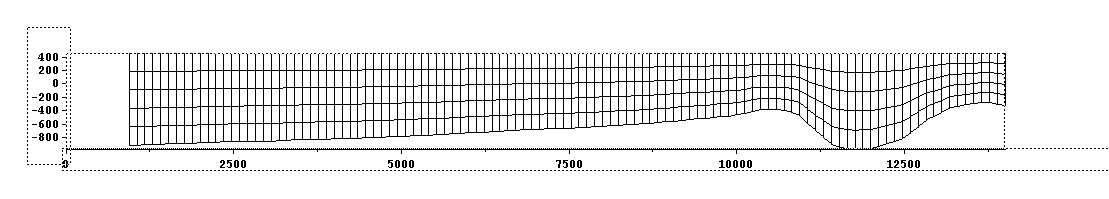
\includegraphics[width=\textwidth]{./graphics/mesh_transformation}
%
\end{center}
\caption
[Effect of the \telkey{MESH TRANSFORMATION}]
{Effect of the \telkey{MESH TRANSFORMATION} keyword -- Value 1: sigma.}
\label{fig:mesh_transf}
\end{figure}

The default value is 1 (Figure \ref{fig:mesh_transf}) and results in a
homogeneous distribution of levels in the vertical direction (classical sigma
transformation). The height of the levels varies depending on the water depth,
all planes can move (except for the bottom). In this case, no programming in
the \telfile{CONDIM} subroutine is required.

A value of 2 (Figure \ref{fig:mesh_transf2}) will allow the user to define the
distribution of levels (e.g. refinement near surface) while maintaining the
levels mobility (sigma transformation with given proportions). The latter
choice implies that the user will program his/her distribution in the
\telfile{CONDIM} subroutine to define the array \telfile{ZSTAR} that describes
the distribution of levels along the vertical as a percentage of the water depth.
Changes to make are:

\begin{itemize}
\item Specifying the variable \telfile{TRANSF\_PLANE} with a value of 2
for every level,

\item Specifying the level distribution along the vertical through the array
\telfile{ZSTAR} which describes the distribution along the vertical as a
percentage of the water depth (the values are between 0. and 1.).
\end{itemize}

For example (Figure \ref{fig:mesh_transf2}):

\begin{lstlisting}[language=TelFortran]
DO IPLAN = 1,NPLAN
  TRANSF_PLANE%I(IPLAN)=2
ENDDO

ZSTAR%R(1)=0.D0
ZSTAR%R(2)=0.02D0
ZSTAR%R(3)=0.1D0
ZSTAR%R(4)=0.4D0
ZSTAR%R(5)=0.8D0

\end{lstlisting}

\begin{figure}[H]%
\begin{center}
%
  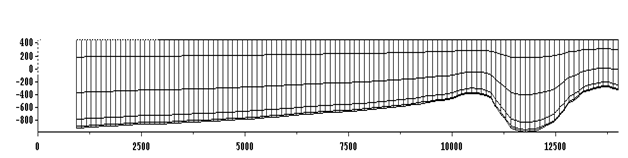
\includegraphics[width=\textwidth]{./graphics/mesh_transformation2}
%
\end{center}
\caption
[Effect of the \telkey{MESH TRANSFORMATION2}]
{Effect of the \telkey{MESH TRANSFORMATION} keyword -- Value 2: zstar.}
\label{fig:mesh_transf2}
\end{figure}

In order to better represent the densimetric stratification areas
(thermoclines, halocline and/or outfall), prescribing a maximum number of
horizontal "levels" (particularly those where the gradients are the highest) is
sometimes suitable. For that purpose, the user can select the value 3 for the
keyword \telkey{MESH TRANSFORMATION}. In this configuration, the user can
freely use the 3 types of level definition available in \telemac{3D} to create
the mesh along the vertical:

\begin{itemize}
\item Fixed levels at a given altitude (correspond to value 3 of the
\telfile{TRANSF\_PLANE} variable, the altitude is specified by the
\telfile{ZPLANE} variable),

\item Irregularly distributed movable levels between two fixed levels
(correspond to value 2 of the \telfile{TRANSF\_PLANE} variable,
the distribution is specified by the \telfile{ZSTAR} variable),

\item Evenly distributed movable levels between two fixed levels (correspond
to value 1 of the \telfile{TRANSF\_PLANE} variable).
\end{itemize}

This latter choice requires the user to make changes in the \telfile{CONDIM}
subroutine:

\begin{itemize}
\item Specifying the variable \telfile{TRANSF\_PLANE} at value 1, 2 or 3
for each level,

\item Specifying the level distribution along the vertical through the array
\telfile{ZSTAR} for levels of type 2,

\item Specifying the level altitude through the array \telfile{ZPLANE} 
for levels of type 3.
\end{itemize}

For example (Figure \ref{fig:mesh_transf3}):
\begin{lstlisting}[language=TelFortran]
DO IPLAN = 1,5
  TRANSF_PLANE%I(IPLAN)=2
ENDDO
ZSTAR%R(1)=0.D0
ZSTAR%R(2)=0.2D0
ZSTAR%R(3)=0.5D0
ZSTAR%R(4)=0.7D0
ZSTAR%R(5)=0.8D0

DO IPLAN = 7,NPLAN
 TRANSF_PLANE%I(IPLAN)=1
ENDDO

TRANSF_PLANE%I(6)=3
ZPLANE%R(6)=0.D0
\end{lstlisting}

\begin{figure}[H]%
\begin{center}
%
  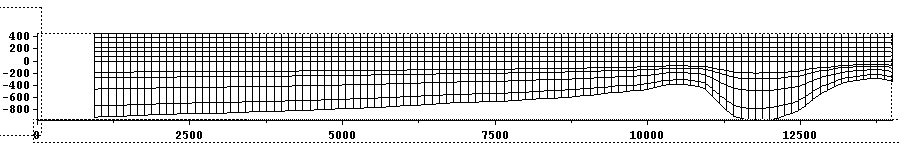
\includegraphics[width=\textwidth]{./graphics/mesh_transformation3}
%
\end{center}
\caption
[Effect of the \telkey{MESH TRANSFORMATION3}]
{Effect of the \telkey{MESH TRANSFORMATION} keyword -- Value 3: user defined.}
\label{fig:mesh_transf3}
\end{figure}

Various programming examples are provided as comments in the \telfile{CONDIM}
subroutine.

The triangular based prismatic elements can optionally be split into
tetrahedrons. This option is enabled using the \telkey{ELEMENT} keyword can
take the value 'PRISM' (default value) or 'TETRAHEDRON'.


\section{Prescribing the initial conditions}

The initial conditions aim at defining the model condition at the beginning of
the simulation.

In case of a continuing computation, the initial conditions are provided at one
time step in the result file of the previous computation (refer to section
\ref{sec:previousfile}).
The mandatory variables (at least the velocity components) when resuming
the computation should then have been stored into the file being used as
\telkey{PREVIOUS COMPUTATION FILE}.

Otherwise, the default initial condition is defined as follows:

\begin{itemize}
\item Free surface set to an elevation equal to 0,

\item Zero velocities,

\item Steady zero active and passive tracers.
\end{itemize}

If that initial condition is not suitable for a computation, then it should be
changed using keywords in the simple cases or through a programming as
described in the subsequent subsections.


\subsection{Prescription through keywords}

In all the cases, the kind of initial conditions is set by the keyword
\telkey{INITIAL CONDITIONS}. That keyword can have one of the following six
values:

\begin{itemize}
\item 'ZERO ELEVATION': Initializes the free surface elevation
to 0 (default value). The initial water depths are then computed from the
bottom depth,

\item 'CONSTANT ELEVATION': Initializes the free surface elevation to the
values as provided by the keyword \telkey{INITIAL ELEVATION}. The initial water
depths are then computed by getting the difference between the free surface
elevation and the bottom depth.  In those areas where the bottom depth exceeds
the initial elevation, the initial water depth is zero,

\item 'ZERO DEPTH': All the water depths are initialized with a zero value
(free surface coinciding with bottom). In other words, the whole domain is
"dry" at the beginning of the computation,

\item 'CONSTANT DEPTH': Initializes the water depths to the value as provided
by the keyword \telkey{INITIAL DEPTH},

\item `TPXO SATELLITE ALTIMETRY': The initial conditions are set using
information provided by the OSU harmonic constants database (TPXO for instance)
in the case of the use of this database for the imposition of maritime boundary
conditions (see subsection \ref{sec:tide}),

\item 'PARTICULAR' or 'SPECIAL': The initial conditions are defined as
programmed by the user in the \telfile{CONDIM} subroutine (refer to the next
subsection).
That procedure should be used whenever the initial conditions of the model do 
not correspond to one of above four cases.
\end{itemize}


\subsection{Prescribing particular initial conditions (Programming the \telfile{CONDIM} subroutine)}
\label{sec:prescr_IC}

The \telfile{CONDIM} subroutine should be programmed whenever the initial
conditions programmed by default are to be modified.

By default, the standard version of the \telfile{CONDIM} subroutine interrupts
the computation if the keyword \telkey{INITIAL CONDITIONS} is set to 'PARTICULAR'
without any actual amendment of the subroutine.

The \telfile{CONDIM} subroutine successively initializes the two-dimensional
variables, then the three-dimensional variables:

\begin{itemize}
\item The water depth,

\item The 3D component of velocities,

\item The active and passive tracers.
\end{itemize}

The user can quite freely fill that subroutine. For instance, he/she can
retrieve information in a formatted or binary file, using the corresponding
keywords.


\subsection{Resuming the computation}

telemac{3D} enables the user to resume a computation by taking as the initial
condition the last time step of a computation which was previously computed on
the same mesh, or possibly with a different number of levels. Thus, some
computational parameters such as the time step, some boundary conditions, the
turbulence model can be modified, or else a computation can be initiated once a
steady state is achieved.

The file to be retrieved shall then inevitably contain all the data required
for \telemac{3D}, i.e. not only the co-ordinates of the $X$, $Y$
and $Z$ computational points which it necessarily contains, but also the
3D velocities and the tracers.

If some variables do not appear in the \telkey{PREVIOUS COMPUTATION
FILE}, then they are automatically set to zero values.  A usual application
consists in using the result of a hydrodynamic computation in order to perform
a tracer transport computation. Generally, the \telkey{PREVIOUS COMPUTATION
FILE} does not include any result for the tracer.

To resume a computation, it is required to use two keywords into the steering
file.

The keyword \telkey{COMPUTATION CONTINUED} should be set to the YES value.

The keyword \telkey{PREVIOUS COMPUTATION FILE} should provide the name of the
file which will provide the initial conditions (default value = 0).

Optionally, the keyword \telkey{RECORD NUMBER FOR RESTART} can be used to
define the record number to read if it is not the last one (defined by a
default value set to 0).

\begin{WarningBlock}{Warning:}
The two-dimensional mesh on which the useful results have been computed should
be strictly identical to the mesh of the case to be handled.
\end{WarningBlock}

Resuming the computation usually leads to small differences in results
compared to the same calculation without interruption. This difference is
mainly due to the fact that the velocity advection is not treated properly at
the first time step, because this operation requires information from the
previous time step. To correct this, the user has a specific recovery procedure
to improve the accuracy of calculations, using double precision format SERAFIN
files:

\begin{itemize}
\item In the first computation, the keyword \telkey{RESTART MODE} is set to
YES, which generates a specific file containing the full information only of
the last time step of the simulation (in particular information on the
advection field of the last time step). The name of this file is specified
using the keyword \telkey{RESTART FILE},

\item In the second computation, this specific file must be used as
\telkey{PREVIOUS COMPUTATION FILE} specifying the \telkey{PREVIOUS COMPUTATION
FILE FORMAT} is 'SERAFIND' (SERAFIN double precision). In this case, the
keyword \telkey{RECORD NUMBER FOR RESTART} cannot be used because the recovery
file only contains the last time step of the simulation.
\end{itemize}

However, it has to be mentioned that even if it is not advisable, the creation
of specific restart file can be done not only SERAFIND format, but also with
any other available format in the TELEMAC system, especially in single
precision. In this case, the keyword \telkey{RESTART FILE FORMAT} (by default
set at 'SERAFIND') must be set to the proper value.

A particular aspect of the resuming technique of computation is the value of
the start time of the second simulation. By default, the start time of the
second calculation is equal to the value of the last time step of restart file.
This can be changed by using the logical keyword \telkey{INITIAL TIME SET TO
ZERO} if the user wants to start from zero (default value is NO).

It is also possible to resume a computation from a 2D results file. This is
generally useful in river hydraulic offering the possibility to initialise the
model in 2D before shifting to 3D simulation. In this case, the horizontal
velocities are considered as constant on the vertical and equal to the 2D
velocities and the vertical velocities are initialised to zero. This
possibility is activated using the \telkey{2D CONTINUATION} logical keyword
(default value = NO). The 2D results file must be given using \telkey{FILE FOR
2D CONTINUATION}. The keyword \telkey{FILE FOR 2D CONTINUATION FORMAT} gives
the format of the file and can takes the following values: `SERAFIN ' (default
value), `SERAFIND' and `MED'.


\section{Prescribing the boundary conditions}
\label{sec:prescr_BC}

The boundary conditions are handled through types of conditions which are
related to the computational variables. The combination of these types (from a
list of possible choices) describes whether the boundary is liquid or solid and
how it should be processed.

In \telemac{3D}, the water depth $H$, the horizontal velocities $U$
and $V$ and the tracers are the only variables which necessarily involve
defining their type of boundary conditions. Those types of boundary conditions
applicable to the vertical velocity and the $k$ and $\epsilon$ functions
are managed by \telemac{3D} by the user directly in the FORTRAN source files of
\telemac{3D} and therefore do not have a type. If the computation takes tracers
into account, then a single type (common to all the tracers) should also be
defined for a given boundary.

Once all the types of the boundary are defined, the user should enter the
related values for the computational variables (at least $H$, $U$ and $V$).

For example, the user may want to set the sea level and leave the velocity
field free (e.g. the tide case). The type of boundary will be: "prescribed
depth and free velocity". The values required for that type are only water
depth at every instant at that boundary. The values of velocities (if they are
entered) are not taken into account for that boundary.

Thus, for each \telemac{3D} boundary, the computational variables (at least
$H$, $U$ and $V$) are necessarily associated with one type
and each type may be associated with one value (either used or not).

The maximum number of boundaries is set to 30 by default but it can be changed
by the user with the keyword \telkey{MAXIMUM NUMBER OF BOUNDARIES}.
This avoids changing the previously hardcoded values (until version 7.0),
which required recompiling the whole package.

After such a description of what is a boundary in \telemac{3D}, we will describe
the types, then the related values.

\subsection{The boundaries in \telemac{3D}}

Water depth is the only two-dimensional variable computed. Its processing at
the boundaries is like that being performed by \telemac{2D}. The boundary points
to be handled are those of the two-dimensional mesh (refer to Figure
\ref{fig:bnd}).

For the other variables (velocities and tracers), the boundary conditions
should be handled over all the boundaries of the three-dimensional mesh which
includes:

\begin{itemize}
\item The lateral boundary points (vertical column points linked to the
boundaries of the two-dimensional mesh), whether it is a liquid or solid
boundary,

\item The points belonging either to the free surface or the bottom.
\end{itemize}

\begin{figure}[H]%
\begin{center}
%
  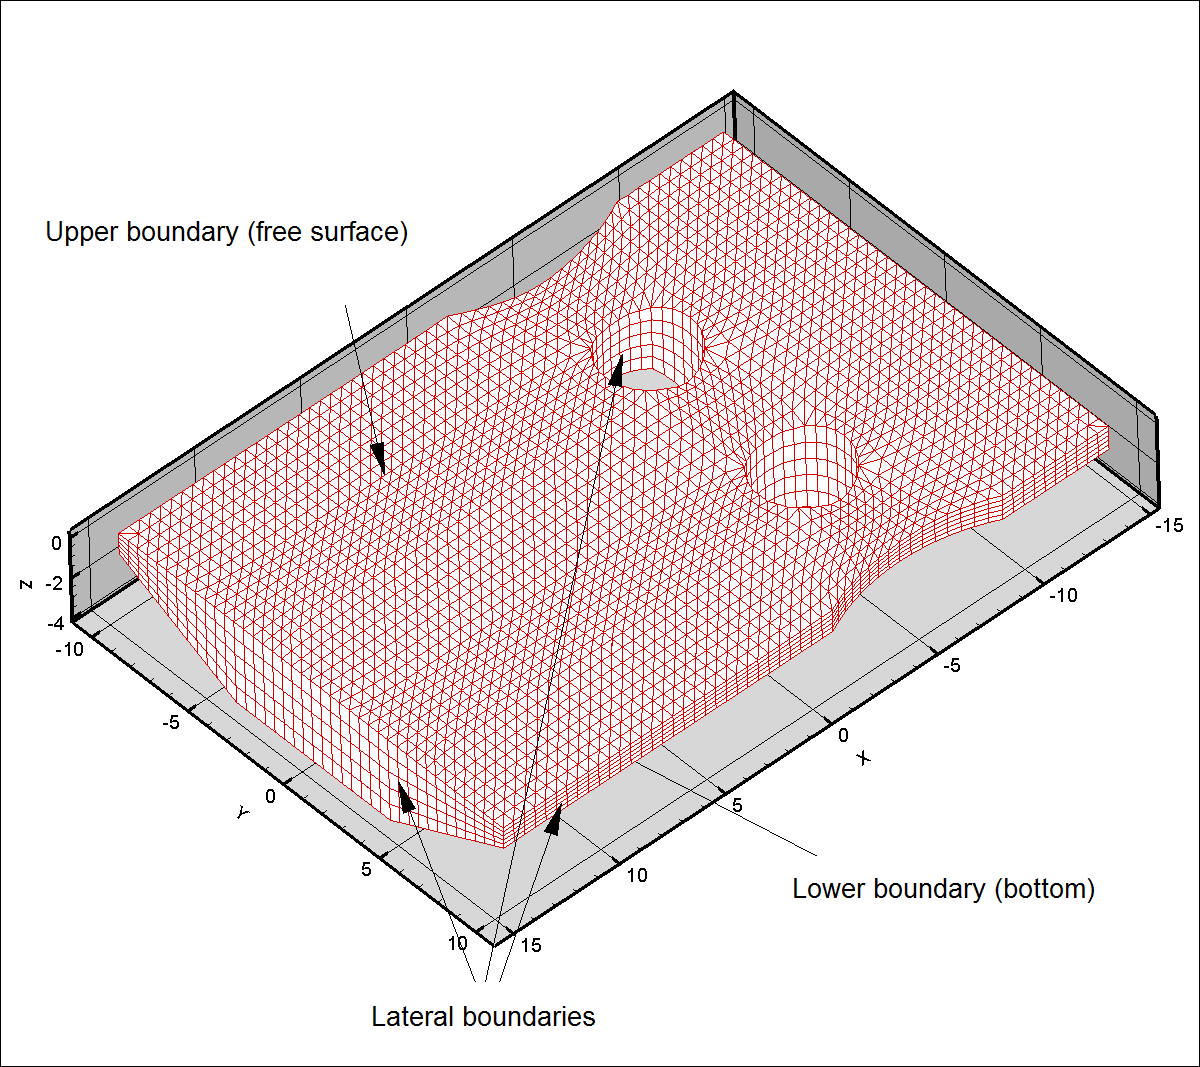
\includegraphics[width=0.7\textwidth]{./graphics/bnd}
%
\end{center}
\caption
[Boudnaries in \telemac{3D}]
{The various boundaries in \telemac{3D} (bridge piers case study).}
\label{fig:bnd}
\end{figure}

By default, \telemac{3D} automatically handles all the surface and bottom points
which do not belong to the side walls. The user, however, can modify them. This
can be done by modifying the FORTRAN sources.

All the remaining points (on the lateral boundaries) are linked to the
two-dimensional mesh boundaries at each horizontal level. Thus, they will be
processed in a similar fashion as in \telemac{2D}. The number of required data,
however, increases so much that a full external handling (either through the
steering file or the boundary conditions file) would become excessively
complex. That is why the range of options offered to the user for dealing with
these boundary conditions is narrower than in \telemac{2D} and definitely implies
programming the sources of the user-available software. The next following
subsections describe the way the boundary nodes are handled.


\subsection{The boundary-related types}

The boundary condition type for $H$, $U$, $V$ and $T$ of the edge points is
read in the boundary conditions file. It can be either modified or directly
defined by the user in the \telfile{LIMI3D} subroutine.

The various types of boundary conditions can be combined in order to prescribe
the conditions of different physical kinds (liquid inflow or outflow in
supercritical conditions, open sea, wall, etc.). Some combinations, however,
are not physical (refer to subsection \ref{sec:descr_bnd} hereinafter).

Some boundary conditions are applicable to such facts as friction at the walls
or wall impermeability. However, the wall definition is ambiguous if one only
retains a definition of point wise boundary conditions. The following
convention is then observed in order to determine the nature of a segment lying
between two different kinds of points: a liquid segment is a segment linking
two liquid-types points. Thus, under that convention, the connecting point
between the shore and the marine boundary (or between the river and the bank)
is preferably of the liquid type. Therefore, liquid + solid = solid

Any sequential arrangement of the boundary types may exist along an outline
(for instance, one may have a liquid boundary with a prescribed depth followed
by a liquid boundaryliquid boundary with a prescribed velocity). The only
condition to be met is that a boundary should consist of at least two points
(it is a computational requirement, a number of at least four points being
highly advisable from a physical point of view).


\subsection{Description of the various types}
\label{sec:descr_bnd}

The type of boundary condition at a given point is provided, in the boundary
conditions file, in the form of four integers which are referred to as
\telfile{LIHBOR}, \telfile{LIUBOR}, \telfile{LIVBOR} and \telfile{LITBOR},
with values which can range from 0 to 6.

The available options are as follows:

\begin{itemize}
\item Depth condition:

\begin{itemize}
\item Prescribed depth liquid boundary: \telfile{LIHBOR}=5,

\item Free depth liquid boundary: \telfile{LIHBOR}=4,

\item Solid boundary (wall): \telfile{LIHBOR}=2.
\end{itemize}
\end{itemize}

It is noteworthy that a depth/rate law is considered as a prescribed depth
condition. The flow rate value should then explicitly be computed, according to
the water depth, by programming the Q3 subroutine.

\begin{itemize}
\item Rate or velocity condition:

\begin{itemize}
\item Prescribed flow rate liquid boundary: \telfile{LIUBOR/LIVBOR}=5,

\item Prescribed velocity liquid boundary: \telfile{LIUBOR/LIVBOR}=6,

\item Free velocity liquid boundary: \telfile{LIUBOR/LIVBOR}=4,

\item Solid boundary with sliding or friction: \telfile{LIUBOR/LIVBOR}=2,

\item Solid boundary with one or two zero velocity components: \telfile{LIUBOR} and/or
\telfile{LIVBOR}=0.
\end{itemize}

\item Tracer condition:

\begin{itemize}
\item Prescribed tracer liquid boundary: \telfile{LITBOR}=5,

\item Free tracer liquid boundary: \telfile{LITBOR}=4,

\item Solid boundary (wall): \telfile{LITBOR}=2.
\end{itemize}
\end{itemize}


\subsection{The boundary conditions file}
\label{sec:bndfile}
That file is provided as standard by MATISSE, Janet, Blue Kenue or \stbtel, but
it can be created or amended by means of FUDAA-PREPRO or a text editor. Each
line of that file is dedicated to one point at the two-dimensional mesh
boundary. The boundary point numbering is the same as that of the file lines,
it first describes the domain outline in the counter clockwise direction, then
the islands in the opposite direction.

The convention being observed in TELEMAC implies that the first liquid boundary
is that which is defined, within the boundary conditions file, by the first two
liquid-typed consecutive numbers. In the example below (channel case study),
the first liquid boundary is defined by the nodes 42-47 (edge numbering) and
corresponds to a prescribed depth (codes 5 4 4 at the beginning of lines). The
second boundary begins at number 76 and ends at number 1 and corresponds to a
prescribed rate (codes 4 5 5).

\begin{lstlisting}[language=bash]
 4 5 5  0.000  0.000  0.000  0.0   2  0.000  0.000  0.000      1     1
 2 2 2  0.000  0.000  0.000  0.0   2  0.000  0.000  0.000      5     2
 2 2 2  0.000  0.000  0.000  0.0   2  0.000  0.000  0.000      6     3
...
 2 2 2  0.000  0.000  0.000  0.0   2  0.000  0.000  0.000     44    41
 5 4 4  0.000  0.000  0.000  0.0   2  0.000  0.000  0.000      2    42
 5 4 4  0.000  0.000  0.000  0.0   2  0.000  0.000  0.000     45    43
 5 4 4  0.000  0.000  0.000  0.0   2  0.000  0.000  0.000     86    44
...
 5 4 4  0.000  0.000  0.000  0.0   2  0.000  0.000  0.000      3    47
 2 2 2  0.000  0.000  0.000  0.0   2  0.000  0.000  0.000     87    48
...
 2 2 2  0.000  0.000  0.000  0.0   2  0.000  0.000  0.000     73    74
 2 2 2  0.000  0.000  0.000  0.0   2  0.000  0.000  0.000     74    75
 4 5 5  0.000  0.000  0.000  0.0   2  0.000  0.000  0.000      4    76
 4 5 5  0.000  0.000  0.000  0.0   2  0.000  0.000  0.000     88    77
...
 4 5 5  0.000  0.000  0.000  0.0   2  0.000  0.000  0.000     89    85
\end{lstlisting}

For each point, and each line in the boundary conditions file, the following
values are entered:

\telfile{LIHBOR, LIUBOR, LIVBOR, HBOR, UBOR, VBOR, AUBOR, LITBOR, TBOR, ATBOR,
BTBOR, N, K}

\begin{itemize}
\item  \telfile{LIHBOR, LIUBOR, LIVBOR} and \telfile{LITBOR} are boundary-typed
integers for each of the variables.

\item \telfile{HBOR} (real) denotes the prescribed depth value when the
\telfile{LIHBOR} value is set to 5,

\item \telfile{UBOR} (real) denotes the prescribed $U$ velocity value when
the \telfile{LIUBOR} value is set to 6,

\item \telfile{VBOR} (real) denotes the prescribed $V$ velocity value when
the \telfile{LIVBOR} value is set to 6,

\item \telfile{AUBOR} denotes the value of the boundary friction coefficient when
the \telfile{LIUBOR} or \telfile{LIVBOR} value is set to 2.
The friction law is then written as:
%TODO: Space between equations
\begin{align}
\upsilon_{T} \frac{dU}{dn} = AUBOR \times U {\rm and/or }
\upsilon_{T} \frac{dV}{dn} = AUBOR \times V
\end{align}
\end{itemize}
The \telfile{AUBOR} coefficient is applicable to the segment included between
the edge point being considered and the next point (in the counter clockwise
direction for the outside outline and in the clockwise direction for the islands).
By default, the \telfile{AUBOR} value is 0.
A friction corresponds to a negative value.
With the $k$-$\epsilon$ model, the value of \telfile{AUBOR} is automatically
computed by \telemac{3D}, the indications in the boundary conditions file will
then be ignored.

\begin{itemize}
\item \telfile{TBOR} (real) denotes the prescribed tracer value when the
\telfile{LITBOR} value is set to 5,

\item \telfile{ATBOR} et \telfile{BTBOR} denote the coefficient values of the
flux law which is written as:
\begin{align}
\upsilon _{T} \frac{dT}{dn} = ATBOR \times T + BTBOR
\end{align}
\end{itemize}
The \telfile{ATBOR} and \telfile{BTBOR} coefficients are applicable to the
segment included between the edge point considered and the next point
(in the counter clockwise direction for the outside outline and in the
clockwise direction for the islands).

\begin{itemize}
\item \telfile{N} denotes the edge point global number,

\item \telfile{K} denotes the point number in the edge point numbering. This
number also represents a node colour (as an integer). This number named
\telfile{BOUNDARY\_COLOR},
can be used in parallel simulations to simplify the implementation of specific
cases. Without particular modification, this value is the rank of the border
point in the global numbering.
For example, a test like \telfile{IF (I.EQ.144) THEN} can be replaced by
\telfile{IF (BOUNDARY\_COLOUR\%I(I).EQ.144) THEN} which is compatible with
the parallel mode. However, this only concerns the 2D mesh (Table
\telfile{BOUNDARY\_COLOUR} is only given for level 1).
Be careful not to modify the last column of the boundary conditions file
that contains this \telfile{BOUNDARY\_COLOUR} table,
when using tidal harmonic constants databases (cf. [6]).
\end{itemize}

As regards the horizontal velocities, all the points in one water column will
have the same type of boundary condition defined by \telfile{LIUBOR} or
\telfile{LIVBOR}.
That principle is intrinsic to the \telemac{3D} formulation. Prescribing a
different type of boundary condition in the vertical direction (e.g. for a
subterranean stream) may, indeed, induce severe inconsistencies with the
hydrostaticity hypothesis and generate, for instance, unrealistic vertical
velocities. It is then advisable that the user will follow that principle.
Nonetheless, the boundary condition type in the vertical direction can be
altered through direct programming in the \telfile{LIMI3D} subroutine.

The so-called \telfile{LIHBOR}, \telfile{LIUBOR} and \telfile{LIVBOR} integers
(which define the boundary type) can assume a value ranging from 0 to 6.
The available options are as follows:

\begin{itemize}
\item Depth-related condition:

\begin{itemize}
\item Prescribed depth liquid boundary: \telfile{LIHBOR=5},

\item Free depth liquid boundary: \telfile{LIHBOR=4},

\item Solid boundary (wall): \telfile{LIHBOR=2},
\end{itemize}

\item Velocity-related condition:

\item Prescribed velocity liquid boundary: \telfile{LIUBOR/LIVBOR=6},

\item Prescribed rate liquid boundary: \telfile{LIUBOR/LIVBOR=5},

\item Free velocity liquid boundary: \telfile{LIUBOR/LIVBOR=4},

\item Solid boundary with sliding or friction: \telfile{LIUBOR/LIVBOR=2},

\item Solid boundary with one or two zero velocity components: \telfile{LIUBOR} and/or
\telfile{LIVBOR=0}.
\end{itemize}

The boundary conditions of physical nature are defined by the relationship
among the types of variables. In most cases, the boundary type can be set by a
mesh generator (e.g. MATISSE or Janet) in the TELEMAC chain. The table
below summarizes the physical relationship among the boundary types.


\begin{tabular}{|p{0.5in}|p{0.5in}|p{0.5in}|p{0.5in}|p{2.0in}|} \hline
LIHBOR & LIUBOR & LIVBOR & LITBOR &  \\ \hline
2 & 2 & 2 & 2 & Solid wall. \\ \hline
2 & 0 & 2 & 2 & Solid wall with zero $U$. \\ \hline
2 & 2 & 0 & 2 & Solid wall with zero $V$. \\ \hline
2 & 0 & 0 & 2 & Solid wall with zero $U$ and $V$. \\ \hline
4 & 4 & 4 & 4 & Free $H$, free velocities, free $T$. \\ \hline
5 & 4 & 4 & 4 & Prescribed $H$, free velocities, free $T$. \\ \hline
5 & 4 & 0 & 4 & Prescribed $H$, free $U$, zero $V$, free $T$. \\ \hline
5 & 0 & 4 & 4 & Prescribed $H$, zero $U$, free $V$, free $T$. \\ \hline
1 & 1 & 1 & 4 & Incident wave, free tracer. \\ \hline
4 & 5 & 5 & 5 & Free $H$, prescribed $Q$, prescribed $T$. \\ \hline
4 & 5 & 0 & 5 & Free $H$, prescribed $Q$ with zero $V$, prescribed $T$. \\ \hline
4 & 0 & 5 & 5 & Free $H$, prescribed $Q$ with zero $U$, prescribed $T$. \\ \hline
4 & 6 & 6 & 5 & Free $H$, prescribed velocities, prescribed $T$.
\\ \hline
5 & 5 & 5 & 5 & Prescribed $H$ and $Q$, prescribed $T$. \\ \hline
5 & 6 & 6 & 5 & Prescribed $H$ and velocities, prescribed $T$. \\
\hline
\end{tabular}


\subsection{Programming the boundary conditions type}

The \telfile{LIMI3D} subroutine can be programmed to handle specific boundary
conditions, for the edge points as well as the surface and bottom points.

That subroutine is called upon each time step. Therefore, it can be used to
change the boundary condition type in time, if required.


\subsection{Prescribing values through keywords}

In most simple cases, the boundary conditions will be prescribed by means of
keywords. However, if the values to be prescribed are variable in time, it is
necessary to program the adequate functions or to use the liquid boundaries
file.

The appropriate keywords to prescribe the boundary values are as follows:

\begin{itemize}
\item \telkey{PRESCRIBED ELEVATIONS}: provided to set the
elevation value of a prescribed height liquid boundary. It is an array which
can contain up to 100 reals, and therefore up to 100 boundaries of that kind
can be handled. The values defined by that keyword overwrite the depth values
read from the boundary conditions file,

\begin{WarningBlock}{Warning:}
The free surface level is set with this keyword, whereas the water depth is set
in the boundary conditions file.
\end{WarningBlock}

\item \telkey{PRESCRIBED FLOWRATES}: provided to set the flow rate value of a
prescribed flow at a liquid boundary. It is an array which can contain up to
100 reals, and therefore up 100 boundaries of that kind can be handled. A
positive value corresponds to a domain inflow rate. The values defined by that
keyword overwrite the velocity values read from the boundary conditions file,

\item \telkey{PRESCRIBED VELOCITIES}: provided to set the velocity value of a
prescribed velocity liquid boundary. The scalar value is the wall normal
velocity. A positive value corresponds to a domain inflow. It is an array which
can contain up to 100 reals, and therefore up 100 boundaries of that kind can
be handled. The values defined by that keyword overwrite the values read from
the boundary conditions file.
\end{itemize}

In addition, several simple rules should be observed:

The boundary type as specified in the boundary conditions files should
obviously be in accordance with the keywords in the steering file (do not
insert the keyword \telkey{PRESCRIBED FLOWRATES} if there are no boundary
points the \telfile{LIUBOR} and \telfile{LIVBOR} of which are set to
5). The keyword, however, is ignored if no type matches it.

For each keyword, the number of specified values should be equal to the whole
number of liquid boundaries, whatever their types may be. When a boundary is
inconsistent with the keyword, then the specified value is ignored (a 0.0 value
or, on the contrary, a very high value such as 999.0 may be systematically
inserted).

For example, in the channel test case, the first boundary (downstream boundary)
is of prescribed level type whereas the second one (upstream boundary) is of
prescribed flow rate type. The steering file contains a sequence of the
following type:

\begin{lstlisting}[language=TelemacCas]
PRESCRIBED ELEVATIONS = 0.5, 0.0
PRESCRIBED FLOWRATES  = 0.0, 50.0
\end{lstlisting}

\subsection{Boundary condition on the bottom}

By default, the boundary condition on the bottom is an impermeable slip
boundary (Neumann condition of the same type as vertical conditions).

However, bottom velocities can be set to zero by using value 2 of the keyword
\telkey{BOUNDARY CONDITION ON THE BOTTOM} (Default value of 1 correspond to a
slip condition). This option is valid only if the vertical mesh is refined at
bottom level.

Since version 7.1, it is possible to prescribe a flux on the bed in TELEMAC-3D
(e.g.: a flow rate on several liquid boundaries placed on the bed).
To do so, it is necessary to define the imposed flow rates using the keywords
\telkey{OPEN BOUNDARY CONDITIONS ON THE BED} set to YES (default value = NO)
and \telkey{PRESCRIBED FLOWRATES ON THE BED} with values following the same
structure as for other prescribed flow rates in the TELEMAC-MASCARET system.
It should be a list of numbers separated by a semi-colon, one number per
liquid boundary on the bed must be given.
The maximum number of boundaries on the bed is set to 30 by default
but it can be changed by the user with the keyword \telkey{MAXIMUM NUMBER OF
BOUNDARIES ON THE BED}.
At the moment, the \telkey{BOUNDARY CONDITIONS FILE} only deals with horizontal
boundaries, therefore the user has to define the liquid boundary on the bed by hand.
This can be done by modifying the subroutine LIMI3D in the \telkey{FORTRAN FILE}.
For example to add a circular boundary of radius 5~m centred around coordinate
(2~000, 2~000)~m, the following modifications can be done:
\begin{lstlisting}[language=TelFortran]
...
!     BOUNDARY CONDITIONS ON VELOCITIES
!     *********************************
!
!     BOTTOM
!     ======
!
!     DEFAULT: IMPERMEABILITY AND LOG LAW (SEE ALSO BORD3D)
!
      IF(BC_BOTTOM.EQ.1) THEN
!
        DO IPOIN2 = 1,NPOIN2
          LIUBOF%I(IPOIN2) = KLOG
          LIVBOF%I(IPOIN2) = KLOG
          LIWBOF%I(IPOIN2) = KLOG
!         USEFUL ? SHOULD NOT BE USED ANYWAY
          UBORF%R(IPOIN2)  = 0.D0
          VBORF%R(IPOIN2)  = 0.D0
          WBORF%R(IPOIN2)  = 0.D0
          IF(SQRT((X(IPOIN2)-2000.D0)**2
     &           +(Y(IPOIN2)-2000.D0)**2)
     &       .LE.50.D0) THEN
            !5: IMPOSED FLOW RATE
            LIUBOF%I(IPOIN2) = 5
            LIVBOF%I(IPOIN2) = 5
            LIWBOF%I(IPOIN2) = 5
            NLIQBED%I(IPOIN2) = 1
            WRITE(LU,*) '========================'
            WRITE(LU,*) 'FOR POINT ',IPOIN2
            WRITE(LU,*) 'BEDFLO',BEDFLO(1)
          ENDIF
        ENDDO
!
...
\end{lstlisting}

In this example, it should be noted that \telfile{NLIQBED\%I(IPOIN2)} = 1
defines the position for the first liquid boundary defined in the steering file.
This is all that needs to be defined by the user to deal with fluxes on the bed.
However, in version 7.1, only constant velocity profile is available.
It should also be noted that it has not been possible to prescribe a tracer
or turbulence yet.

\subsection{Using the liquid boundaries file}
\label{sec:liqbnd}
In case of time variable values, which are nonetheless constant in space along
the relevant liquid boundary, the prescription can be made using the liquid
boundaries file (as an alternative to programming).

It is a user-edited text file the name of which should be given by the keyword
\telkey{LIQUID BOUNDARIES FILE}. That file has the
following format:

\begin{itemize}
\item The optional line(s) begin(s) with the sign $\#$ (1st character on the
line) will be treated as comments,

\item It should contain a header line beginning with \telfile{T} for identifying
the supplied time dependent value(s) within that file. The identification is
performed through mnemonic means which are identical to the variable names:
\telfile{Q} for the flow rate, \telfile{SL} for the level, \telfile{U} and
\telfile{V} for the velocities and \telfile{TR} for the
tracer. These characters are directly followed by an integer in between
brackets which is used to specify the current boundary. That line is
necessarily followed by another line indicating the unit of the variables
(lines of comments can be inserted, but the line of units should be present).
The units are given for information only and \telemac{3D} does not handle the
conversion of units (thus, the user has to enter the values using the standard
unit),

\item The values to be prescribed are provided through a sequence of lines the
format of which should be consistent with the identification line. The time
value should be increasing and the last time value supplied should be higher
than or equal to the value of the last time step, otherwise the computation is
suddenly interrupted.
\end{itemize}

Upon the retrieval of that file, \telemac{3D} performs a linear interpolation in
order to compute the value prescribed at a particular time step. The value
which is actually prescribed by the code is printed on the check listing.

An example of a liquid boundaries file is given below.

\begin{lstlisting}[language=bash]
#  Example of liquid boundaries file
#  2 boundaries are managed
#
T Q(1) SL(2)
s m3/s m
0. 0. 135.0
25. 15. 135.2
100. 20. 136.
500. 20. 136.
\end{lstlisting}

In that example, the flow rate is prescribed at the first boundary and the free
surface is prescribed at the second boundary.


\subsection{Prescribing values through programming}

Still in the case of time variable values that are constant in time along the
liquid boundary processed, the prescription can be made simply by programming
particular functions:

\begin{itemize}
\item \telfile{VIT3} function for prescribing a velocity,

\item \telfile{Q3} function for prescribing a flow rate,

\item \telfile{SL3} function for prescribing an elevation.
\end{itemize}

Functions \telfile{Q3, VIT3} and \telfile{SL3} are similarly programmed.
In each case, the user knows the time, the boundary rank (e.g. to determine
whether the first or the second prescribed flow rate boundary is processed).
By default, the functions prescribe values that are read from the boundary
conditions file or provided by the keywords.

For instance, the body of function \telfile{Q3} used to prescribe a flow rate
ramp for the first 1,000 seconds from 0 to 400~m${}^{3}$/s can take such a form as:

\begin{lstlisting}[language=TelFortran]
IF (AT.LT.1000.D0) THEN
  Q3 = 400.D0 * AT/1000.D0
ELSE
  Q3 = 400.D0
ENDIF
\end{lstlisting}

Or

\begin{lstlisting}[language=TelFortran]
Q3 = 400.D0 * MIN(1.D0,AT/1000.D0)
\end{lstlisting}

\subsection{Stage-discharge curves}
\label{sec:discharge}
\telemac{3D} allows managing liquid boundaries for which the prescribed water
elevation value is a function of local flow rate. This situation is encountered
particularly in river hydraulics.

First, it is necessary to specify which boundaries are concerned with the
keyword \telkey{STAGE-DISCHARGE CURVES}. This keyword provides an integer value
for each boundary. This value can be:

\begin{itemize}
\item 0: no stage-discharge curves (default),

\item 1: elevation as a function of local flow rate.
\end{itemize}

The keyword \telkey{STAGE-DISCHARGE CURVES FILE} provides the name of the text
file containing information about the curves. An example is shown below:

\begin{lstlisting}[language=bash]
#
#  STAGE-DISCHARGE CURVE BOUNDARY 1
#
Q(1)      Z(1)
m3/s      m
61.       0.
62.       0.1
63.       0.2
#
#  STAGE-DISCHARGE CURVE BOUNDARY 2
#
Z(2)      Q(2)
m         m3/s
10.       1.
20.       2.
30.       3.
40.       4.
50.       5.
\end{lstlisting}

The order of curves has no significance. The column order can be reversed, as
is the case for the second boundary in the example.
Lines beginning with \telfile{\#} are comments.
The lines defining the units are mandatory but the units are not checked.
The number of points of each curve is completely free and need not be
the same for each curve.

Warning: at initial conditions, the flow at the exit can be null. The initial
level must correspond to that of the calibration curve otherwise a sudden
change is imposed. To avoid extreme situations, the curve should be limited to
a certain level of flow rate. In the example of boundary 1 above, the flow
rates below 61~m${}^{3}$/s generate a water elevation of 0~m above the flow of
63~m${}^{3}$/s to produce an elevation equal to 0.2~m.

\subsection{Prescribing complex values}

If the values to be prescribed vary in both space and time, then a programming
in the \telfile{BORD3D} subroutine becomes necessary, since that subroutine can
be used to prescribe the values in a node wise way.

That subroutine describes all the liquid boundaries (loop on \telfile{NPTFR2}).
For each boundary point, it determines the boundary type in order to prescribe
the adequate value (velocity, elevation or flow rate).
\telfile{BORD3D} programming to prescribe a flow rate, however, hardly makes
any sense, since the flow rate value is generally known for the whole boundary
rather than on each boundary segment.

If a prescribed flow rate inlet is surrounded by walls with an adherence, then
the corner velocities are cancelled.

Note that, the \telfile{BORD3D} subroutine also makes it possible to prescribe
the complex boundary values of the tracers.

\subsection{Prescribing a profile}


\paragraph{Horizontal profile}

When processing a prescribed flow rate or prescribed velocity boundary, the
user has the keyword \telkey{VELOCITY PROFILES} to specify which "horizontal"
velocity profile should be prescribed by \telemac{3D}. The following options are
possible:

\begin{itemize}
\item 1: The profile is normal and homogeneous along the boundary (default
option),

\item 2: The values of $U$ and $V$ are read from the boundary
conditions file (\telfile{UBOR} and \telfile{VBOR} values).
In case of a prescribed flow rate, these values are multiplied by a constant
in order to get the desirable flow rate,

\item 3: The velocity vector is normal to the boundary and its norm is read
from the boundary conditions file as the \telfile{UBOR} value. In case of a
prescribed flow rate, that value is multiplied by a constant in order to get
the desirable flow rate,

\item 4: The velocity vector is normal to the boundary and its norm is
proportional to the square root of the water depth,

\item 5: The velocity vector is normal to the boundary and its norm is
proportional to the square root of a virtual water depth computed from lowest
point of the free surface on the boundary.
\end{itemize}

\paragraph{ Vertical profile}

When processing a prescribed flow rate or prescribed velocity boundary, the
user has the keyword \telkey{VELOCITY VERTICAL PROFILES} to specify which
"vertical" velocity profile should be prescribed by \telemac{3D}. The options for
that keyword are:

\begin{itemize}
\item 0: programmed by the user,

\item 1: constant (default value for all the liquid boundaries),

\item 2: logarithmic.
\end{itemize}

The user programming is done within the \telfile{VEL\_PROF\_Z} subroutine.

Activating the keyword \telkey{DYNAMIC BOUNDARY CONDITION} (default value =
FALSE) also enables to prescribe a velocity at the free surface coherent with
the dynamic boundary condition.

\subsection{Thompson conditions}

In some cases, not all the necessary information concerning the boundary
conditions is available. This is usual for coastal domains where only the
values of the sea level on several points are known. This kind of model is
referred to as an ``under-constrained'' model.

To solve this problem, the Thompson method uses the characteristics method to
calculate the missing values. For example, \telemac{3D} will compute the velocity
at the boundary in the case of a prescribed elevation.

This method can also be used for ``over-constrained'' models. In this case,
the user specifies too much information at the boundary. If the velocity
information and the level information are not consistent, too little or too
much energy is going into the model. For this, the Thompson method computes a
new value for the velocity and performs small adjustments to cancel the
inconsistencies in the information.

For this, the user can use the keyword \telkey{OPTION FOR LIQUID BOUNDARIES},
which offers two values (the user must specify 1 value for every open
boundary):

\begin{itemize}
\item 1: strong setting (default value for all boundaries),

\item 2: Thompson method.
\end{itemize}

Taking a simplified view, it may be said that, in the case of the first
option, the values are ``imposed'', in the case of the second option, the
values are ``suggested''.

However it is important to note that, given the two-dimensional aspect, the
Thompson method can only be used in the case of a zero velocity gradient
imposed on the vertical (uniform velocity along the vertical).


\subsection{Tidal harmonic constituents databases}
\label{sec:tide}


\subsubsection{General parameters}

To prescribe the boundary conditions of a coastal boundary subject to tidal
evolution, it is generally necessary to have the information characterizing
this phenomenon (harmonic constants). One of the most common cases is to use
the information provided by large scale models.

4 databases of harmonic constants are interfaced with \telemac{3D}:

\begin{itemize}
\item The JMJ database resulting from the LNH Atlantic coast TELEMAC model
by Jean-Marc JANIN,

\item The global TPXO database and its regional and local variants from
the Oregon State University (OSU),

\item The regional North-East Atlantic atlas (NEA) and the global atlas
FES (e.g. FES2004 or FES2012...) coming from the works of Laboratoire
d'Etudes en Géophysique et Océanographie Spatiales (LEGOS),

\item The PREVIMER atlases.
\end{itemize}

However it is important to note that, in the current version of the code, the
latter 2 databases are not completely interfaced with \telemac{3D} and their use
is recommended only for advanced users.

The keyword \telkey{OPTION FOR TIDAL BOUNDARY CONDITIONS} activates the use of
one of the available database when set to a value different from 0
(the default value 0 means that this function is not activated). 
Since version 7.1, this keyword is an array of integers separated by semicolons
(one per liquid boundary) so that the user can describe whether tidal boundary
conditions should be computed or not (e.g. a weir) on a liquid boundary. 
When this keyword is activated, every tidal
boundary is treated using the prescribed algorithms for the boundaries with
prescribed water depths or velocities, with the same option for tidal boundary
conditions (the values not equal to 0 have to be the same).
The databases provide only a single value of the
depth-averaged velocity, thus \telemac{3D} prescribes the same value of the
velocity at each point along the vertical (for more information, see
Méthodologie pour la simulation de la marée avec la version 6.2 de \telemac{2D}
et \telemac{3D}, C.-T. Pham et al., EDF report H-P74-2012-02534-FR
\cite{Pham2012}).

The database used is specified using the keyword \telkey{TIDAL DATA BASE} which
can take the values:

\begin{itemize}
\item 1: JMJ,

\item 2: TPXO,

\item 3: MISCELLANEOUS (LEGOS-NEA, FES20XX, PREVIMER...).
\end{itemize}

Depending on the database used, some keywords have to be specified.

\begin{itemize}
\item If using the JMJ database, the name of the database (typically bdd\_jmj)
is given by the keyword \telkey{ASCII DATABASE FOR TIDE} and the corresponding
mesh file is specified using the keyword \telkey{TIDAL MODEL FILE},

\item If using the TPXO database, the name of the water level database is given
by the keyword \telkey{BINARY DATABASE 1 FOR TIDE} (for example h\_tpxo7.2) and
the name of the velocity database is given by the keyword \telkey{BINARY
DATABASE 2 FOR TIDE} (for example u\_tpxo7.2). Moreover, it is possible to
activate an interpolation algorithm of minor constituents from data read in the
database using the logical keyword \telkey{MINOR CONSTITUENTS INFERENCE},
activation not done by default.
\end{itemize}

The keyword \telkey{OPTION FOR TIDAL
BOUNDARY CONDITIONS} specifies the type of tide to prescribe. The default value
0 means no prescribed tide or that the tide is not treated by standard
algorithms. Value 1 corresponds to prescribing a real tide considering the time
calibration given by the keywords \telkey{ORIGINAL DATE OF TIME} (YYYY~; MM~;
DD format) and \telkey{ORIGINAL HOUR OF TIME} (HH~; MM~; SS format). Other
options are the following, available for every tidal database (JMJ,
TPXO-type from OSU, LEGOS-NEA, FES, PREVIMER \ldots).
They are called “schematic tide” for values from 2 to 6:

\begin{itemize}
\item 2: exceptional spring tide (French tidal coefficient approximately equal
110),

\item 3: mean spring tide (French tidal coefficient approximately equal 95),

\item 4: mean tide (French tidal coefficient approximately equal 70),

\item 5: mean neap tide (French tidal coefficient approximately equal to 45),

\item 6: exceptional neap tide (French tidal coefficient approximately equal
to 30),

\item 7: real tide (before 2010 methodology, only available with JMJ).
\end{itemize}

In the case of options 2 to 6 (schematic tides), the boundary conditions are
imposed so that the reference tide is approximately respected.
In order to shift the phases of the waves of the tidal constituents so that
the computation starts close to a High Water, two keywords are available.
If using a TPXO-type tidal database from Oregon State University, the keyword
\telkey{GLOBAL NUMBER OF THE POINT TO CALIBRATE HIGH WATER} has to be filled
with the global number of the point (between 1 and the number of boundary
nodes in the 2D mesh) with respect to which the phases are shifted
to start with a high water (mandatory, otherwise the computation stops).
This point has to be a maritime boundary node.
If using one of the other tidal databases (JMJ, NEA/FES, PREVIMER) the keyword
\telkey{LOCAL NUMBER OF THE POINT TO CALIBRATE HIGH WATER} should be filled in
with the local number between 1 and the number of tidal boundary points of the
\telkey{HARMONIC CONSTANTS FILE}; If not filled in (default value = 0), a value
is then automatically calculated. However, it is usually necessary to
wait for the second or third modelled tide in order to overcome the
transitional phase of start-up of the model. It is also necessary to warn the
user that the French tidal coefficients shown are approximate.

During a simulation, data contained in the tidal database are interpolated on
boundary points. When using the JMJ database, this spatial interpolation can
be time consuming if the number of boundary points is important, and is not yet
available in case of parallel computing. It is therefore possible to generate a
file containing harmonic constituents specific to the model treated. The
principle is at a first step, to perform a calculation on a single time step
whose only goal is to extract the necessary information and to generate a file
containing for each boundary point of the model, the harmonic decomposition of
the tidal signal. Subsequent calculations directly use that specific file
rather than directly addressing to the global database. The harmonic constants
specific file is specified using the keyword \telkey{HARMONIC CONSTANTS FILE},
this file is an output file in the first calculation, and an input file in
subsequent calculations.


\subsubsection{Horizontal spatial calibration}

In order to perform the spatial interpolation of the tidal data, it is
imperative to provide to \telemac{3D} information on the spatial positioning of
the mesh model relative to the grid of the tidal database. To do this, the user
has two keywords:

The first keyword specifies the geographic system used to establish the
coordinates of the 2D mesh of \telemac{3D}. This keyword \telkey{GEOGRAPHIC
SYSTEM}, which has no default value, may take the following values:

\begin{itemize}
\item 0: User Defined,

\item 1: WGS84 longitude/latitude in real degrees,

\item 2: WGS84 UTM north,

\item 3: WGS84 UTM south,

\item 4: Lambert,

\item 5: Mercator projection.
\end{itemize}

The second keyword is used to specify the area of the geographic system used to
establish the coordinates of the 2D mesh of \telemac{3D}. This keyword
\telkey{ZONE NUMBER IN GEOGRAPHIC SYSTEM} which has no default value, may take
the following values:

\begin{itemize}
\item 1: Lambert 1 north,

\item 2: Lambert 2 center,

\item 3: Lambert 3 south,

\item 4: Lambert 4 Corsica,

\item 22: Lambert 2 extended,

\item 93: Lambert 93,

\item $X$: UTM zone value of the WGS84 ($X$ is the number of the
zone).
\end{itemize}

If using the Lambert 93 projection, the user has to copy the file provided
in the tide examples of \telemac{2D} called gr3df97a.txt which is used
for the conversion in the Lambert 93 projection.
The keyword \telkey{LAMBERT 93 CONVERSION FILE} has to indicate the path
and the name of the gr3df97a.txt file.

\subsubsection{Calibration of the information}

The transfer of information between a large scale model and the boundaries of
a more local model generally requires calibration.

To do this, the user has three keywords:

\begin{itemize}
\item The keyword \telkey{COEFFICIENT TO CALIBRATE SEA LEVEL} (default real
value 0.0) is used to calibrate the mean tide level (the harmonic decomposition
of information provided by the various databases are used to generate the tidal
signal oscillating around mean tide level). The calibration of the mean tide
level must obviously be made depending on the altimetric reference used in the
model,

\item The keyword \telkey{COEFFICIENT TO CALIBRATE TIDAL RANGE} (default real
value 1.0) is used to specify a calibration coefficient applied on the
amplitude of the tidal wave. This coefficient is applied to the amplitude of
the overall signal, and not on the amplitude of each of the elementary waves,

\item The keyword \telkey{COEFFICIENT TO CALIBRATE TIDAL VELOCITIES} (default
real value 999,999.0) is used to specify the coefficient applied on velocities.
The default value (999, 999.0) means that the square root of the value
specified by the keyword \telkey{COEFFICIENT TO CALIBRATE TIDAL RANGE} tidal is
used.
\end{itemize}

For more information, the reader may refer to methodological guide for tide
simulation with version 6.2 \cite{Pham2012}.



%----------------------------------------------------------------------------------------
%	CHAPTER 5: Physical setup
%----------------------------------------------------------------------------------------

\chapter{Physical setup of the hydrodynamic computation}

In addition to the general setup given in the steering file, a number of
physical parameters may or should be specified upon a simulation.


\section{Hydrostatic pressure hypothesis}

Firstly, it should be specified whether one wants to use the hydrostatic
pressure hypothesis or not. That choice is made using the keyword
\telkey{NON-HYDROSTATIC VERSION} which, by default, has been set to YES since
version 8.0.
As a reminder, the hydrostatic pressure hypothesis
(\telkey{NON-HYDROSTATIC VERSION} = NO)
consists in simplifying the
$W$ vertical velocity, ignoring the diffusion, advection and other
terms. Therefore, the pressure at a point is only related to the weight of the
overlying water column and to the atmospheric pressure at the surface. Without
the hydrostatic pressure hypothesis (\telkey{NON-HYDROSTATIC VERSION} = YES),
\telemac{3D} solves a $W$ vertical velocity equation which is similar to
the $U$ and $V$ equations, with the additional gravity term.


\section{Modelling turbulence}

The Reynolds numbers ($Re = U.L/\upsilon$) reached for tidal
flows or in an estuary are excessively high and illustrate basically turbulent
flows ($L$, the scale of eddies, for example, assumes the value of water
depth $h$ for a vertically homogeneous flow). For such a kind of flow,
the turbulence-induced momentum prevails (in relation to the molecular
diffusion). That diffusion is strictly defined by a tensor which could be
anisotropic.

The concept of eddy scale, however, is spatially constrained by the horizontal
and vertical scales of the modelled domain. At sea, for example, a one
kilometre long cape can generates eddies the dimensions of which are
horizontally related to that scale. Vertically, however, the eddy size is
constrained by the water depth or even more by possible effects of
stratifications. Synthetically, a common practice consists in separating the
vertical and horizontal turbulence scales which are not relevant to the same
dynamics for the standard applications of \telemac{3D}. That involves defining
horizontal as well as vertical viscosities rather than a single viscosity. On
the open sea, for instance, the horizontal and vertical viscosities differ by
several orders of magnitude.

Thus, the implementation of \telemac{3D} requires defining two models of
horizontal and vertical turbulence (\telkey{HORIZONTAL TURBULENCE MODEL},
\telkey{VERTICAL TURBULENCE MODEL}).

Turbulence modelling is an awkward task and \telemac{3D} offers the user several
approach options which are different, but also increasingly complex, and are
applicable to velocities as well as to active and passive tracers.

The Von Karman constant and Prandtl number (ratio between eddy viscosity and
eddy diffusivity) can be changed with the keywords \telkey{KARMAN CONSTANT}
(default value = 0.4) and \telkey{PRANDTL NUMBER} (default value = 1.).

\subsection{Constant viscosity}

The simplest turbulence model consists in using a constant viscosity
coefficient (option for parameters: 1="CONSTANT VISCOSITY", default value). In
that case, the latter includes the effects of molecular viscosity and
dispersion (refer to Theoretical note \cite{Hervouet2007}).
The horizontal and vertical
turbulent viscosities are then constant throughout the domain. The global
(molecular + turbulent) viscosity coefficients are provided by the user by
means of the keywords \telkey{COEFFICIENT FOR HORIZONTAL DIFFUSION OF
VELOCITIES} and \telkey{COEFFICIENT FOR VERTICAL DIFFUSION OF VELOCITIES}, set
by default to $10^{-6}$.

The value of that coefficient has a definite effect on both size and shape of
the recirculations and eddies. A low value will tend to only dissipate the
small-sized eddies, a high value will tend to dissipates large-sized
recirculations. The user shall then carefully select that value according to
the case studied. Usually, that value becomes a model calibration data by
comparison with measurements. Besides, it is worth mentioning that a value
bringing about the dissipation of recirculations of a smaller than two mesh
cell extent has nearly no influence on the computation (i.e. there is a
threshold beyond which the viscosity or turbulence value has substantially no
effect).

\telemac{3D} makes it possible to get a space- and time-variable coefficient.
The \telfile{VISCOS} subroutine will necessarily be programmed.
Within that subroutine, geometrical information, basic hydrodynamic
information (water depth, velocity components) and time are made available
to the user.

That option theoretically aims at enabling the user to define the turbulent
viscosity by programming the  \telfile{VISCOS} subroutine.

\subsection{Mixing length (vertical model)}

The user also has the opportunity to use a vertical mixing length model
(\telkey{VERTICAL TURBULENCE MODEL}: 2="MIXING LENGTH"). The vertical
diffusivity of velocities is then automatically computed by \telemac{3D} by means
of the selected mixing length model taking or not taking the effects of density
into account. The mixing length model expresses the turbulent viscosity (or
diffusion coefficient) as a function of the mean velocity gradient and the
mixing length (Prandtl's theory):
%TODO:See how to handle where
\begin{align}
\nu =L_{m}^{2} \sqrt{2D_{ij} D_{ij}} \textrm{ where }  D_{ij} =\frac{1}{2}
\left(\frac{\partial \bar{U}_{i} }{\partial x_{j} }
      +\frac{\partial \bar{U}_{j}}{\partial x_{i} } \right)
\end{align}

Due to that choice, the user should enter the following options for the mixing
length model (\telkey{MIXING LENGTH MODEL}):

\begin{itemize}
\item  1: Prandtl (default). Standard Prandtl's model. That formulation suits
such flows with a strong barotropic component as the tidal flows,

\item  3: Nezu and Nakagawa. Nezu and Nakagawa model,

\item  5: Quetin \cite{Quetin1977}. Better representation of wind drift.
In windy weather, a surface boundary layer is formed and viscosity decreases,

\item  6: Tsanis \cite{Tsanis1989}. Better representation of wind drift.
\end{itemize}

The graph below shows the variations of the mixing length for the various models.

\begin{figure}[H]%
\begin{center}
%
  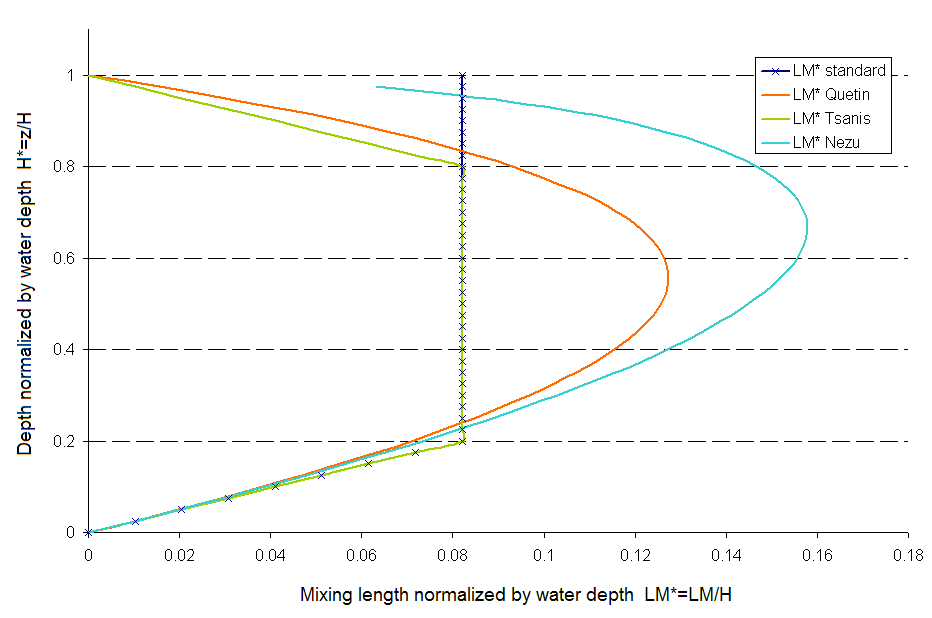
\includegraphics[width=\textwidth]{./graphics/mixing_lengths}
%
\end{center}
\caption
[Mixing lengths versus depth]
{Mixing lengths versus depth.}
\label{fig:mix_len}
\end{figure}

In the presence of a vertical density gradient, the environment stability
(respectively the instability) hinders (enhances) the vertical exchanges of
mass and momentum.

In order to quantify the effects of the gravity terms in the turbulent power
balance, the dimensionless Richardson number is commonly used. It is a local
number the value of which can obviously be different at each flow point.

In order to take the mixture reduction into a stable stratified flow into
account, a damping law is introduced into the turbulence model according to the
Richardson number. The user can set the damping function through the keyword
\telkey{DAMPING FUNCTION}. The available options are:

\begin{itemize}
\item  0: nothing (default value),

\item  1: user-performed; Law programming in the \telfile{DRIUTI} subroutine,

\item  2: Viollet,

\item  3: Munk and Anderson.
\end{itemize}

The graph below illustrates the variation of the Munk and Anderson damping
function according to the Richardson number for velocity and salinity. In the
case of a stable stratification, the pressure fluctuations more readily
transmit a momentum flux than a mass flux and the diffusion coefficient becomes
higher for the velocities than for the mass.

\begin{figure}[H]%
\begin{center}
%
  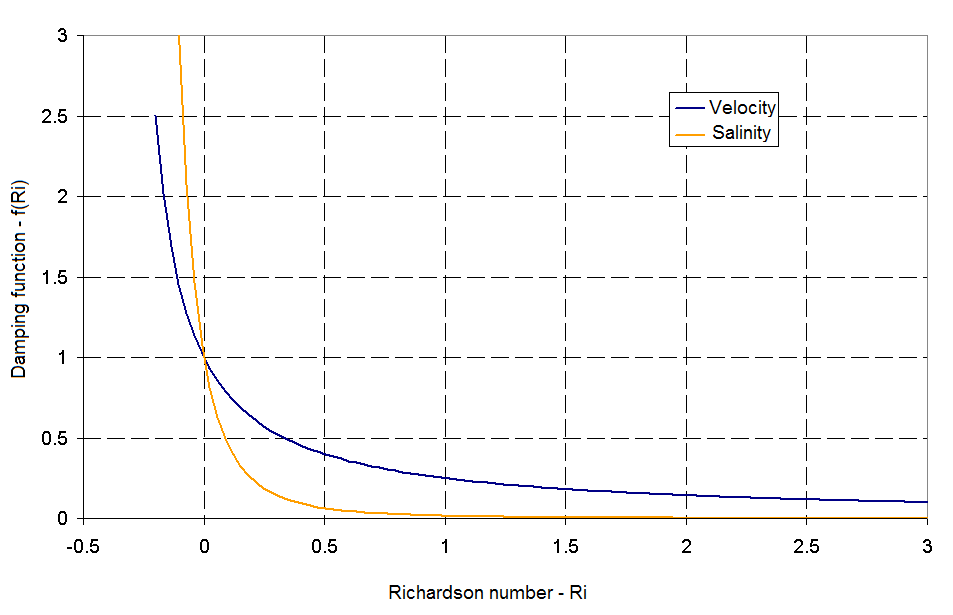
\includegraphics[width=\textwidth]{./graphics/munk_anderson}
%
\end{center}
\caption
[Munk and Anderson damping function]
{Munk and Anderson damping function.}
\label{fig:munk_anderson}
\end{figure}

When using the mixing length model, the user can also configure the calculation
of the vertical derivative of the velocities with the keyword \telkey{VERTICAL
VELOCITY DERIVATIVES}. Default value 1 corresponds
to a vertical derivative that is linear. Value 2 activates a logarithmic
computation between the bottom and 0.2 times the water depth. This allows
getting better results when modelling the velocity profile near the bottom.
This algorithm is implemented in the subroutine \telfile{VISCLM}.


\subsection{Smagorinsky}

That option is activated by setting the horizontal or vertical turbulence
model to 4 (Smagorinsky).

The Smagorinsky scheme is recommended, in particular, in the presence of a
highly non-linear flow \cite{Smagorinsky1963}.


\subsection{$k$-$\epsilon$}

\telemac{3D} gives an opportunity to use the so-called $k$-$\epsilon$
model as proposed by Rodi and Launder for solving the turbulence equations.
That model is activated by setting the keywords of turbulence models
(\telkey{HORIZONTAL TURBULENCE MODEL} and \telkey{VERTICAL TURBULENCE MODEL})
to the value 3.

The $k$-$\epsilon$ model is defined through a couple of equations
solving the balance equations for $k$ (turbulent energy) and $\epsilon$
(turbulent dissipation). Applying the $k$-$\epsilon$ model often
requires using a finer two-dimensional mesh than the constant viscosity model
and then increases the computation times.

For detailed information about the formulation of the mixing length and
$k$-$\epsilon$ models, the user can refer to the \telemac{3D} Theoretical
Note.

Strictly speaking, except for the constant viscosity model, the diffusion
coefficient should be equal to the molecular diffusion of water:

\begin{lstlisting}[language=TelemacCas]
COEFFICIENT FOR HORIZONTAL DIFFUSION OF VELOCITIES = 1.D-6
COEFFICIENT FOR VERTICAL DIFFUSION OF VELOCITIES = 1.D-6
\end{lstlisting}

The default value of that viscosity may have to be increased to ensure a minimum
diffusion, especially during the first time steps of the computation.

There are two options to compute the lateral boundary conditions of $k$ and
$\epsilon$ (in subroutine KEPCL3) with the keyword
\telkey{OPTION FOR THE BOUNDARY CONDITIONS OF K-EPSILON}:
\begin{itemize}
\item 1 = No turbulence ($k$ and $\epsilon$ takes the minimum values
\telfile{KMIN} and \telfile{EMIN} defined in subroutine \telfile{CSTKEP}),
which is the default value,
\item 2 = Hans and Burchard’s formula (introduced in version 7.0).
\end{itemize}

Since version 8.1, \telemac{3D} can be coupled with the GOTM library
(General Ocean Turbulence Model).
It enables to use a turbulence model library over the vertical by setting
the keyword \telkey{VERTICAL TURBULENCE MODEL} to 6="STANDARD GOTM"
and providing an ASCII file containing GOTM parameters with the keyword
\telkey{GOTM STEERING FILE}.
An example of such a file can be found in the \telemac{3D} example
stratification.
As GOTM is a 1DV water column model, the turbulence model can only be used over
the vertical and the user can choose another turbulence model in the $x$ and
$y$ directions with the keyword \telkey{HORIZONTAL TURBULENCE MODEL}.

\section{Setting up the friction}

The bottom or sidewall friction reflects the continuity of the constraint at
the fluid-solid interface. Knowing the constraint involves knowing the flow in
the vicinity of the bottom. The turbulence models provide a modelling for that
flow.

The constraint can be written in several forms:
\begin{align}
\vec{\tau } & = \mu \frac{\partial \vec{U}}{\partial n}
            = -\frac{1}{2} \rho C_{f} \sqrt{U^{2} +V^{2} } \vec{U}\\
            & = -\rho U^{*2}
\end{align}
where $U^{*}$ denotes the friction, $C_{f}$ - a dimensionless friction, $U$ -
the velocity of current recorded far enough from the wall.

The friction condition is then provided:

\begin{itemize}
\item  Either by a turbulence model which indicates the constraint through a
friction velocity formulation,

\item  Or by the knowledge of the friction coefficient $C_{f}$ and the related
velocity $U$ (here, the vertically-averaged velocity). That approach will then
use the Chézy, Strickler, Manning\dots  laws.
\end{itemize}

The same approach is adopted for both sidewalls and bottom.


\subsection{Bottom friction}

The friction law used for the bottom friction modelling is set by the keyword
\telkey{LAW OF BOTTOM FRICTION} which can assume the following values:

\begin{itemize}
\item  0: No friction,

\item  1: Haaland law,

\item  2: Chézy law,

\item  3: Strickler law,

\item  4: Manning law,

\item  5: Nikuradse law (default value since version 8.1).
\end{itemize}

As regards the 1-5 values, the value of the friction coefficient corresponds to
the selected law, and shall be given by means of the keyword \telkey{FRICTION
COEFFICIENT FOR THE BOTTOM}. Obviously, that only holds true if the friction is
constant in both space and time. The default value for that parameter is 0.01
which corresponds to 1~cm for a Nikuradse law (old default value = 60 for Chézy
law until version 8.0).

The computation of turbulent constraint at the bottom depends on the velocity
profile above the bottom (within the boundary layer). The profile depends on
the ratio of the wall asperity size to the viscous sub-layer thickness (for
further details, refer to the Theoretical Manual). When the asperities are
larger than the viscous sub-layer thickness, the latter cannot be established
and the friction regime is rough. On the other hand, when there is a viscous
sub-layer, the friction regime is smooth.

The computation of the turbulent constraint depends on the keyword
\telkey{TURBULENCE REGIME FOR THE BOTTOM}. The available options are:

\begin{itemize}
\item  1: smooth regime,

\item  2: rough (default value).
\end{itemize}

In smooth friction regime conditions,~the friction law is not used and the
constraint is computed from Reichard law of velocity profile (a law giving the
friction velocity value $U^{*}$.

In rough friction regime conditions and for the bottom friction laws 0, 2, 3
and 4, the constraint is computed from the friction velocity $U^{*}$ and its
relation to the $C_{f}$ coefficient. For law 5, the friction velocity is
computed from the velocity profile within the logarithmic layer and from the
asperity size $k_{s}$ (\telkey{FRICTION COEFFICIENT FOR THE BOTTOM}).


\subsection{Sidewall friction}

The friction law used to model the sidewall friction is set by the keyword
\telkey{LAW OF FRICTION ON LATERAL BOUNDARIES} which can take the following
values:

\begin{itemize}
\item  0: No friction (default value),

\item  5: Nikuradse law.
\end{itemize}

The size of asperities (which is used in the Nikuradse law) is given by the
\telkey{FRICTION COEFFICIENT FOR LATERAL SOLID BOUNDARIES} (default value
0.01~m since version 8.1, old default value = 60! until version 8.0).

The friction is activated using the keyword \telkey{TURBULENCE REGIME FOR
LATERAL SOLID BOUNDARIES}. The available options are:

\begin{itemize}
\item  1: smooth regime,

\item  2: rough (default value).
\end{itemize}

That option changes the formulation of the velocity profile and consequently,
the friction velocity. See previous section for more information.

\section{Punctual source terms}
\label{sec:srcfile}
\telemac{3D} offers an opportunity to place momentum sources or sinks in any
point of the domain.

The user has two options to place horizontally the various sources:
\begin{enumerate}
\item  using the keywords \telkey{ABSCISSAE OF SOURCES} and
\telkey{ORDINATES OF SOURCES}. They are arrays of reals giving the co-ordinates
of sources, in meters. Actually, \telemac{3D} will position a source at the
closest mesh point to the point as specified by these keywords. The software
will determine itself the number of sources according to the number of values
given to each keyword,
\item using the keyword \telkey{GLOBAL NUMBERS OF SOURCE NODES}.
This is an array of integers which contains the global numbers of nodes
in the 2D mesh that correspond to source point locations. The software
will determine itself the number of sources according to the number of values
given to the keyword.
\end{enumerate}

The vertical positioning of the sources is done using the keyword
\telkey{ELEVATIONS OF SOURCES}. \telemac{3D} places the sources on the nearest
mesh level. In this case, it is recommended to use fixed levels at sources
elevations in order to avoid unwanted vertical movement of the sources during
the simulation. Also note that the sources cannot be placed on the bottom level
(level number 1). This is to ensure an impermeable bottom boundary.

At each source, the user should specify the liquid flow rate. That liquid flow
rate is given (in m${}^{3}$/s) using the keyword \telkey{WATER DISCHARGE OF
SOURCES}.

In case of sources with variable characteristics, the user can then either use
specific programming in the \telfile{T3D\_DEBSCE} subroutine (and
\telfile{T3D\_TRSCE} in the presence of tracer), or use the source file whose
name is given by the keyword \telkey{SOURCES FILE}.
This file has exactly the same structure as the liquid
boundary file. An example is shown below with two sources and two tracers.
Between two specified times, the information used by \telemac{3D} at sources is
obtained by linear interpolation.

\begin{lstlisting}[language=TelemacCas]
#
#  FLOW RATES ANS TRACERS CONCENTRATIONS AT SOURCES 1 ET 2
#
#  T IS THE TIME
#
#  Q(1) IS FLOW RATE AT SOURCE 1
#  Q(2) IS FLOW RATE AT SOURCE 2
#
#  TR(1,1) IS TRACER 1 CONCENTRATIONS AT SOURCE 1
#  TR(1,2) IS TRACER 2 CONCENTRATIONS AT SOURCE 1
#  TR(2,1) IS TRACER 1 CONCENTRATIONS AT SOURCE 2
#  TR(2,2) IS TRACER 2 CONCENTRATIONS AT SOURCE 2
#
#
T     Q(1)     TR(1,1)    TR(1,2)    Q(2)      TR(2,1)   TR(2,2)
s     m3/s        C          C        m3/s        C         C
0.     0.        99.        20.       0.         30.       40.
2.     1.        50.        20.       2.         30.       20.
4.     2.        25.        80.       4.         30.       20.
\end{lstlisting}

Besides, \telemac{3D} is capable of taking into account an injection velocity (in
m/s) at the sources in the dynamic equations. By default, the injection takes
places without any momentum input. The user may prescribe a particular
velocity. If the latter is constant throughout the simulation, then its value
can be given using the keywords \telkey{VELOCITIES OF THE SOURCES ALONG X},
\telkey{VELOCITIES OF THE SOURCES ALONG Y} and
\telkey{VELOCITIES OF THE SOURCES ALONG Z}. Otherwise, the user
should program the SOURCE subroutine in order to amend \telfile{USCE} (for the
velocity at sources along $X$) and \telfile{VSCE} (for the velocity at sources
along $Y$). The user can use the time and all the parameters of the sources
within that subroutine.

From a theoretical point of view, complete mass conservation can only be ensured
if the source is treated as a Dirac function and not as a linear function.
The type of treatment is indicated by the user with the keyword
\telkey{TYPE OF SOURCES}, which can have a value of 1 (linear function,
default value) or 2 (Dirac function).
It should be noted that in the second case, the solutions are of course
less smoothed.
It is the same implementation as in \telemac{2D} and the Dirac option is
recommended with a big number of sources.
The maximum number of sources is set to 20 by default but it can be changed
by the user with the keyword \telkey{MAXIMUM NUMBER OF SOURCES}.
This avoids changing the previously hardcoded values (until version 7.0),
which required recompiling the whole package.

\section{Setting up the water-atmosphere exchanges}

\subsection{The wind}

\telemac{3D} can be used to simulate flow while taking into account the influence
of a wind blowing on the water surface. The logical keyword \telkey{WIND} is
used first of all for determining whether this influence is taken into account
and if so, the coefficient is then provided with the keyword
\telkey{COEFFICIENT OF WIND INFLUENCE} (default value =
$1.55 \times 10^{-6}$ since version 8.0). Lastly, if the
wind is constant in time and space, wind speed in directions X and Y is
supplied with the keywords \telkey{WIND VELOCITY ALONG X} and \telkey{WIND
VELOCITY ALONG Y}. Default values for these three coefficients are 0.

The coefficient of wind influence hides complex phenomena. In fact, the
influence of the wind depends on the smoothness (or, lack of it) of the free
surface and the distance over which it acts (called the ``fetch''). The
coefficient value can be obtained from many different formulas.

This is the formula used by the Institute of Oceanographic Sciences (United
Kingdom):

\begin{tabular}{ll}
if $\overrightarrow{U}_{vent} < 5$ m/s & $a_{vent}  = 0.565 \times 10^{-3}$ \\
if $5 < \overrightarrow{U}_{vent}  < 19.22$ m/s & $a_{vent} = (- 0.12 + 0.137\overrightarrow{U}_{vent} ) 10^{-3}$ \\
if $\overrightarrow{U}_{vent} > 19.22$ m/s & $a_{vent} = 2.513 \times 10^{-3}$ \\
\end{tabular}

This formula can be activated by setting the keyword
\telkey{COEFFICIENT OF WIND INFLUENCE VARYING WITH WIND SPEED} to YES
(default value is NO).

The parameter \telkey{COEFFICIENT OF WIND INFLUENCE} asked for by \telemac{3D}
is: $a_{vent} (\rho_{air} / \rho)$ and not only $a_{vent}$.
$\rho_{air}$ is approximately 1.2 kg/m$^3$ and $\rho$
is approximately 1,000 kg/m$^3$. Thus it is necessary to divide the value of
$a_{vent}$ by 1,000 to obtain the value of the \telemac{3D} keyword.
The default value of \telkey{COEFFICIENT OF WIND INFLUENCE} has been set to
$1.55 \times 10^{-6}$ since version 8.0.

The whole formulation used to consider the wind effects, through the keyword
\telkey{COEFFICIENT OF WIND INFLUENCE} (refer to the Theoretical Note for the
definition of that coefficient), on the surface flows is fully stated in the
\telfile{BORD3D} subroutine.

If the wind velocity is space- or time-variable, the user should modify the
\telfile{METEO} subroutine.

\begin{WarningBlock}{Warning:}
The \telfile{METEO} subroutine is provided to define the wind velocity and
direction even though they are space- or time-variable.
The \telfile{BORD3D} subroutine describes the law of wind-induced drift
of water bodies.
\end{WarningBlock}

If there are tidal flats or dry zones in the domain, the wind may trigger
unphysical velocities as it becomes the only driving term in the equations. To
avoid this, the influence of the wind is cancelled below a threshold value of
depth, with the key-word \telkey{THRESHOLD DEPTH FOR WIND} (default value at
1~m).


\subsection{The temperature}

Air temperature may be specified using the keyword \telkey{AIR TEMPERATURE} if
it is constant in time and space.


\subsection{The pressure}

The influence of air pressure is taken into account from the moment when the
keyword \telkey{AIR PRESSURE} is set to YES (the default value is
NO). The value of that pressure is directly set in the \telfile{METEO} subroutine.
By default, the latter initializes a pressure of $10^5$ Pa ($\approx$ 1 atm) over
the whole domain.


\subsection{Rain or evaporation}

The modelling of the influence of precipitation or evaporation is activated
with the logical keyword \telkey{RAIN OR EVAPORATION}. The value of the
contribution or the loss of water at the surface is specified using the keyword
\telkey{RAIN OR EVAPORATION IN MM PER DAY} which default value is 0. (a
negative value reflects an evaporation).

In case of calculation with consideration of tracers, it is possible to specify
the contribution related to the rain with the keyword \telkey{VALUES OF TRACERS
IN THE RAIN} (default value is 0.). It is important to note that, in the case
of evaporation, no tracer is taken into account in the water loss, which is
incorrect if the tracer is the temperature.

\subsection{Atmosphere-water exchange models}

Before version 7.0, heat exchange between water and atmosphere could have been
done with a linearised formula of the balance of heat exchange fluxes at the
free surface. An example of an exchange with a constant atmosphere temperature
and a constant sea salinity was given as standard (as comments) through a
direct programming in the \telfile{BORD3D} subroutine.

A much more elaborated model has been introduced in \telemac{3D}.
Since version 7.2, this model has been integrated in \waqtel and
\telemac{3D} has to be coupled with \waqtel to activate it
(\telkey{COUPLING WITH} = 'WAQTEL'), with
\telkey{WATER QUALITY PROCESS} = 11 (since version 8.0, 5 previously)
in the \waqtel steering file.
This module calculates the complete balance of exchanged fluxes involved:

\begin{itemize}
\item  The solar radiation,

\item  The atmospheric radiation,

\item  The water radiation,

\item  The latent heat due to evaporation,

\item  The sensitive heat of conductive origin.
\end{itemize}

It takes into account the solar radiation penetration in the water column.

The choice of the heat exchange model can be done with the keyword
\telkey{ATMOSPHERE-WATER EXCHANGE MODEL} in the \waqtel steering file
(default value = 0: no exchange
model). Value 1 will use with the linearised formula at the free surface,
whereas value 2 will use with the model with complete balance.

These calculations require additional data (wind magnitude and direction, air
temperature, atmospheric pressure, relative humidity, nebulosity and rainfall,
all these variables may vary in time) in a standard format, rather defined
in the \telkey{ASCII ATMOSPHERIC DATA FILE} of the \telemac{3D} steering file,
see the example "heat\_exchange".
The format may be changed but the user has to change the
implementation of the reading and the interpolation of the meteorological data.
When using the complete module, evaporation is calculated by \telemac{3D}, but
the user has to provide rainfall data with units homogeneous with length over
time.

The main developments of this module are implemented in the module
\telfile{EXCHANGE\_WITH\_ATMOSPHERE}.

Some physical parameters or formulae can be changed with the helps of some
keywords in the \waqtel steering file (default values are the mean values): e.g.
the type of sky related to the luminosity of the site with the \waqtel keyword
\telkey{LIGHTNESS OF THE SKY} (1: very pure sky, 2: mean pure sky or 3:
industrial zone sky) or the \telkey{FORMULA OF ATMOSPHERIC RADIATION}
(1: Idso and Jackson (1969), 2: Swinbank (1963) which is the default formula,
3: Brutsaert (1975) or 4: Yajima Tono Dam (2014)).
Some other physical parameters have been hard-coded in the module, often
imposed as the mean value: e.g. the type of cloud (cirrus,
cirro stratus, alto cumulus, alto stratus, stratus), but these values can be
changed in the module \telfile{EXCHANGE\_WITH\_ATMOSPHERE}).

Because the site of a study may not be equipped with local wind measurements
and these kinds of data are available at a different location, possibly far
from the studied site, a wind function is used. This is a linear function with
a single coefficient of calibration $b:f(U_{2}) = b(1+U_{2}$) where $U_{2}$ is
the wind velocity at 2~m high.

To get the wind velocity at 2~m high from classical wind data at 10~m high, a
roughness length of ${z}_{0}~=~0.0002$~m has been chosen in the code,
that leads to $U_{2} \approx 0.85 U_{10}$. This value
of 0.85 (or the roughness length) may be changed by the user if needed.

Examples of solar radiation penetration are given in the
\telfile{CALCS3D\_THERMICV} subroutine. Two laws are suggested: the first one
uses the \emph{in situ} measurements of Secchi length and is
recommended if available; the second one uses two exponential laws that may be
difficult to calibrate and require an estimation of the type of water from
turbidity.

Except for the coefficient to model the penetration of solar radiation in the
water column, the parameter $b$ that appears in the wind function is the
single calibration parameter of this module. Its value is given by the keyword
\telkey{COEFFICIENT TO CALIBRATE THE ATMOSPHERE-WATER EXCHANGE MODEL}
in the \waqtel steering file (default
value = 0.0025 but recommended values are between 0.0017 and 0.0035). This
keyword is both used for the linearised formula at the free surface and the
model with complete balance (values 1 and 2 for the keyword
\telkey{ATMOSPHERE-WATER EXCHANGE MODEL} in the \waqtel steering file).


\section{Astral potential}

When modelling large maritime areas, it is sometimes necessary to take into
account the effect of astral forces generating tide inside the area. For this,
the user has several keywords at his disposal.

First of all, the logical keyword \telkey{TIDE GENERATING FORCE} (default value
NO) allows these phenomena to be taken into account.

The keyword \telkey{LONGITUDE OF ORIGIN POINT} must be positioned at the right
value.

Lastly, the two keywords \telkey{ORIGINAL DATE OF TIME} (format YYYY;MM;DD) and
\telkey{ORIGINAL HOUR OF TIME} (format HH;MM;SS) must be used to give the
beginning time of the simulation.  This information is necessary for \telemac{3D}
to compute the respective position of the moon and the sun.

\section{Consideration of wave driven currents}

It is possible to take into account the wave driven currents by retrieving
information calculated by a wave propagation module of the TELEMAC modelling
system (mainly \tomawac but also \artemis). In the current version,
only taking into account a steady state is possible. The procedure is as
follows:

\begin{itemize}
\item  Perform a calculation of wave propagation on the same mesh as the
\telemac{3D} calculation requesting the storage of the driving forces. In the
case of \tomawac, the variables \telfile{FX} and \telfile{FY},

\item  Get the wave results file and provide its name through the keyword
\telkey{BINARY DATA FILE 1},

\item  Activate the keyword \telkey{WAVE DRIVEN CURRENTS},

\item  Fill the keyword \telkey{RECORD NUMBER IN WAVE FILE}. This value
corresponds to the iteration number stored in the wave file which must be taken
into account by \telemac{3D}. Usually, this is the last iteration stored, by
default this number is set to 1. The name of the variables to read is "FORCE
FX" and "FORCE FY", but this can be changed within the TRISOU subroutine.
\end{itemize}

In the current version of \telemac{3D}, this driving force is considered as being
constant over the vertical.

If the user wishes to take into account several results of the wave propagation
module (e.g. to take into account changes in the level of the sea), FORTRAN
programming is required.

\section{Other physical parameters}

When modelling large domains, the influence of the Coriolis force of inertia
has to be taken into account. This is done by activating the logical keyword
\telkey{CORIOLIS} (which is set to NO by default). In such a case, the value of
the Coriolis coefficient (refer to the Theoretical Note) is defined by the
keyword \telkey{CORIOLIS COEFFICENT} (default value is 0.). The latter should
be computed according to latitude l through the formula:

\begin{itemize}
\item  $2\, \omega \, \sin \, \left(\lambda \right)$ where $\omega$ is the
Earth's rotational velocity of $7.27 \times {10}^{-5}$ rad/s and $\lambda$ is the
average latitude of the model.
\end{itemize}

In the case of very large domains such as portions of oceans, it is necessary
to carry out a simulation with spherical coordinates, in which case the
Coriolis coefficient is adjusted automatically at each point of the domain (see
10.3), by activating the keyword \telkey{SPHERICAL COORDINATES}.

\telemac{3D} additionally offers the opportunity to set the acceleration due to
gravity (keyword \telkey{GRAVITY ACCELERATION} which, by
default, is set to 9.81~m/s${}^{2}$).


%----------------------------------------------------------------------------------------
%	CHAPTER 6: Numerical setup
%----------------------------------------------------------------------------------------

\chapter{Numerical setup of the computation}

The numerical setup is comparatively common to a hydrodynamic computation alone
or with a tracer. Thus, in the following sections of this chapter, the
numerical parameters as applied to the solution of a tracer equation are
integrated into the hydrodynamic parameters.

\section{General setup}

\telemac{3D} solves the Navier-Stokes equations in several stages, possibly
through the three stages of the fractional step method (see the theoretical
note). The first stage consists in finding out the advected velocity components
by only solving the convection terms of the momentum equations. The second
stage computes, from the advected velocities, the new velocity components by
taking into account both diffusion and source terms of the momentum equations.
These two solutions enable to get an intermediate velocity field. The third
stage computes the water depth from the vertical integration of the continuity
equation and momentum equations only including the pressure-continuity terms.
This step is called the propagation step.

The user can activate or deactivate, either globally or individually, some of
these stages.


\subsection{Advection step}
\label{sec:advstep}
Whether the convection terms will be considered or not will be determined by
means of the logical keyword \telkey{ADVECTION STEP} (default
value YES). However, even though that keyword is set to YES, then some
advection terms can be deactivated by means of the following complete keywords
(value 0 = "NO ADVECTION "):

\begin{itemize}
\item \telkey{SCHEME FOR ADVECTION OF VELOCITIES}: for the advection of
velocities,

\item \telkey{SCHEME FOR ADVECTION OF DEPTH}: for taking the advection of
depth into account (default value = 5 which is the single choice and now
mandatory),

\item \telkey{SCHEME FOR ADVECTION OF K-EPSILON}: for the advection of power
and turbulent dissipation,

\item \telkey{SCHEME FOR ADVECTION OF TRACERS}: for the advection of tracers
(one value per tracer).
\end{itemize}

See section \ref{sec:advection} for more information on the possible choices.

\subsection{Diffusion step}
\label{sec:difstep}

%Deleted keyword in v7.3
%Whether the diffusion terms are taken into account or not is established by
%means of the logical keyword \telkey{DIFFUSION STEP} (default value YES).
%However, even though that keyword is set to YES, then
Some diffusion terms can be deactivated by means of the following complete
keywords by the following keywords:

\begin{itemize}
\item \telkey{SCHEME FOR DIFFUSION OF VELOCITIES},

\item \telkey{SCHEME FOR DIFFUSION OF TRACERS} (one value common to all tracers),

\item \telkey{SCHEME FOR DIFFUSION OF K-EPSILON}.
\end{itemize}

The 0 value at each keyword cancels the diffusion, whereas the 1 value
(default value) leads to the implicit calculation of diffusion.

%Deleted keyword in v7.3
%For the treatment of the diffusion, two choices are possible for the keyword
%\telkey{OPTION FOR THE DIFFUSION}. The default value 1 means an implicit
%treatment whereas the value 2 means an uncoupled treatment between the
%horizontal diffusion and the vertical diffusion.


\subsection{Propagation step}

%Deleted keyword in v7.3
%The velocity and water depth propagation processes are taken into account by
%the logical keyword \telkey{PROPAGATION STEP} (default value YES).

Since the version 6.0 of TELEMAC, the propagation step (for velocity and water
depth) is necessarily treated with \telemac{2D} "wave equation" option.

The propagation step can be linearized by activating the keyword
\telkey{LINEARIZED PROPAGATION} (default value = NO) particularly when one
conducts a case study for which an analytical solution in the linearized case
is available. It is then necessary to set the water depth around which the
linearization is performed by means of the keyword \telkey{MEAN DEPTH FOR
LINEARIZATION} (default value 0.).

With the "wave equation" option, the keyword
\telkey{FREE SURFACE GRADIENT COMPATIBILITY} can be used.
A value lower than 1. (which is the default value) makes
it possible to delete the spurious oscillations of the free surface, but
slightly alters the consistency between the water depth and the velocities in
the continuity equation.

When using the non-hydrostatic version, it is possible to enable the dynamic
pressure term in treatment of the wave equation. This option is enabled by the
logical keyword \telkey{DYNAMIC PRESSURE IN WAVE EQUATION} but it leads a
dilemma:

\begin{itemize}
\item If the keyword is set to YES, the dynamic pressure gradient is taken
into account when calculating the evolution of the water depth (advantage), but
the evolution of the water depth is not known when calculating the dynamic
pressure (disadvantage),

\item If the keyword is set to NO (which is the default value), the dynamic
pressure is calculated taking into account the evolution of the water depth
(advantage) but it is not taken into account in the calculation of the water
depth (disadvantage).
\end{itemize}

Therefore, when the effect of the dynamic pressure is important (nonlinear
waves), it is recommended to set this keyword to YES in combination with
setting sub-iterations for nonlinearities (see test case NonLinearWave).


\section{The advection scheme}
\label{sec:advection}
The procedure for taking the advection terms into account is individualized
for each of the variables liable to be processed. It has previously been
explained that the zero option corresponds to a deactivation of the term.


\subsection{Advection of the three-dimensional variables}

The advection schemes of the three-dimensional variables (i.e.
all the variables except the water depth) are (for further details about these
options, the reader shall refer to the Theoretical Note):

\begin{itemize}
\item 0: Deactivation,

\item 1: Method of characteristics. That method involves mutually independent
advection and diffusion steps. The method consists in writing that the value of
the advected variable is equal to the value of the same variable in the
previous instant traced back on the path travelled during the time step,

\item 2: Explicit scheme + SUPG (Streamline Upwind Petrov Galerkin). That
method uses test functions which are deformed in the direction of the current
for the variational method,

\item 3: Explicit Leo Postma scheme,

\item 4: Explicit scheme + MURD (Multidimensional Upwind Residual
Distribution) N scheme,

\item 5: Explicit scheme + MURD PSI scheme,

\item 13: Explicit Leo Postma scheme for tidal flats,

\item 14: Explicit scheme + MURD (Multidimensional Upwind Residual
Distribution) N scheme for tidal flats.
\end{itemize}

The latter five schemes are primarily recommended for the tracers, since they
are advantageous in being conservative and monotonic, i.e. they do not generate
any numerical oscillation. On the other hand, they are more diffusive than
SUPG. In that respect, scheme 5 is an improvement to scheme 4, being less
diffusive perpendicularly to the flow but quite obviously somewhat more
computation time-consuming. Nevertheless, it is still globally less
time-consuming than SUPG.

Distributive schemes (options 3, 4, 5, 13 or 14) are schemes whose stability is
conditioned by a Courant number less than 1. When using one of these schemes,
at each time step, \telemac{3D} performs a test for checking the Courant number
point by point. In case it exceeds the value 1, \telemac{3D} will automatically
execute sub-iterations to satisfy the stability criterion. However, if the
number of sub-iterations exceeds 100, \telemac{3D} considers that the treatment
of the advection term is problematic and the calculation is interrupted,
printing an error message in the list control.

The default value for both
\telkey{SCHEME FOR ADVECTION OF VELOCITIES} and
\telkey{SCHEME FOR ADVECTION OF K-EPSILON}
is 5 since version 8.1
(old value until version 8.0 was 1 i.e. method of characteristics). 
Combined with the new default values of the keywords
\telkey{SCHEME OPTION FOR ADVECTION OF VELOCITIES} = 4
and \telkey{SCHEME OPTION FOR ADVECTION OF K-EPSILON} = 4,
that means that a LIPS scheme is used (see \ref{sec:MURD}).
That value is advisable, since it is satisfactory in many instances.
% and is by far the fastest.
The default value for the tracers is still 5 and also with the default value of
\telkey{SCHEME OPTION FOR ADVECTION OF TRACERS} equal to 4. It is the
most reliable scheme, since the "mass" conservation of the active tracers is a
frequently essential point in \telemac{3D}.

Since version 6.0, the value concerning the water depth advection scheme is
ignored by \telemac{3D}. The optimum advection scheme is automatically selected
by the software (conservative scheme).

According to the schemes used, the mass conservation can be improved by
performing sub-iterations. That consists in an updating, for one given time
step, both advective field and propagative field during several sub-iterations.
Upon the first sub-iteration, the field of velocities is yielded by the results
achieved during the previous time steps. Through that procedure, the
non-linearities can be taken into account in a better way and the mass
conservation can be significantly improved in the cases of schemes 2 and 3. The
number of sub-iterations is set by the keyword \telkey{NUMBER OF SUB ITERATIONS
FOR NON LINEARITIES}, the default value of which is 1 (also refer to the
Theoretical Note).

The SUPG scheme can be configured using specific keywords (see \ref{sec:supg}).

The MURD schemes present several options described in \ref{sec:MURD}.

\subsection{Configuration of the SUPG scheme}
\label{sec:supg}
When using the SUPG method, the user must determine the type of upwinding
desired using the keyword \telkey{SUPG OPTION} which is an array of
4 integers related, to the velocity, the water depth, tracers and
$k$-$\varepsilon $ model respectively.
Default value = (1;0;1;1).

The possible values are:

\begin{itemize}
\item 0: no upwinding,

\item 1: upwinding with the conventional SUPG method, that is to say, the
upwinding is 1,

\item 2: upwinding with the modified SUPG method, that is to say, the
upwinding is equal to the Courant number.
\end{itemize}

In theory, option 2 is more accurate when the Courant number is less than 1,
but should not be used when the latter is important. Thus, option 2 should be
used in models for which the Courant number remains low. If the Courant number
cannot be estimated, it is strongly recommended to use option 1 (which can be
considered as the most universal).

\subsection{Configuration of the MURD schemes}
\label{sec:MURD}
The N and PSI residual distribution schemes present different options that allow
to increase the accuracy of the numerical scheme or to deal with tidal flats.
The keyword \telkey{SCHEME OPTION FOR ADVECTION OF VELOCITIES} (which can be
found also for $k$-$\epsilon$ and tracers) specifies the desired option and must
be used coupled with the keyword
\telkey{SCHEME FOR ADVECTION OF VELOCITIES} = 4 (or 5).
It can be set to:
\begin{itemize}
 \item 1: explicit scheme,
 \item 2: first order predictor-corrector scheme,
 \item 3: second order predictor-corrector scheme,
 \item 4: locally semi-implicit predictor-corrector scheme
(for tidal flats): LIPS (default value since version 8.1).
\end{itemize}
The default value for \telkey{SCHEME OPTION FOR ADVECTION OF VELOCITIES} is
4 (i.e. LIPS) since version 8.1 which works with tidal flats (old value = 1
i.e. explicit scheme until version 8.0).
If there are no tidal flats in the domain, using option 2 (first order
predictor-corrector scheme) may accelerate the computation but it does not
work with tidal flats.

Like in \telemac{2D}, the predictor-corrector schemes need an additional
parameter which represents the number of iterations for every time step
(or sub-time step) to converge to the solution.
The keyword \telkey{NUMBER OF CORRECTIONS OF DISTRIBUTIVE SCHEMES}
(default value = 1) plays this role and it is useful for unsteady cases.
For quasi-steady flows, the number of corrections does not have a large impact
on the solution, so it can be set to 0.
On the other hand, for unsteady flows, it is suggested to set the keyword
\telkey{NUMBER OF CORRECTIONS OF DISTRIBUTIVE SCHEMES} = 2 (at least),
which is a good compromise between accuracy and computational time.
Indeed, by increasing the number of corrections, the scheme is more accurate but
the CPU time rapidly increases.\\
The keyword \telkey{NUMBER OF SUB-STEPS OF DISTRIBUTIVE SCHEMES} can be
activated only for locally semi-implicit predictor-corrector schemes (LIPS).
The default value is 1.
As the keyword mentions, it allows to subdivide the time step given by the user
in the steering file, into several sub-steps.
Again, it produces an effect on the precision of the scheme and it is convenient
to set this keyword in order to have Courant numbers not too large (around 1).

\subsection{Configuration of the weak characteristics}

When choosing the method of characteristics, two forms can be used with the
keyword \telkey{OPTION FOR CHARACTERISTICS}:

\begin{itemize}
\item 1: the strong form (by default),

\item 2: the weak form.
\end{itemize}

None of them are recommended for the advection of tracers because they are not
mass conservative. The weak form will decrease the diffusion. If the keyword
\telkey{MASS-LUMPING FOR WEAK CHARACTERISTICS} = 1. (default value = 0. i.e. no
mass-lumping), monotonicity of the scheme appears. This weak form should be
more conservative than the strong form. The \telkey{NUMBER OF GAUSS POINTS FOR
WEAK CHARACTERISTICS} defines the number of Gauss points used to compute the
weak characteristics. One single choice is possible for \telemac{3d}: 6 points
(default value).
%The bigger the number is, the more conservative the scheme is, but the higher the
%computational costs are.


\section{Specific parameters in the non-hydrostatic version}

The application of the software \telkey{NON-HYDROSTATIC VERSION} (default = YES)
requires that complementary keywords be defined.

An equation for vertical velocity is initially solved in a same way as the
$U$ and $V$ components. That equation is only written with the
hydrostatic pressure which, under that hypothesis, is cancelled out with the
gravity term. The convection scheme in that equation is identical to that
chosen for $U$ and $V$ (keyword \telkey{SCHEME FOR ADVECTION OF
VELOCITIES}).
%The solution of the linear system (for the diffusion step
%integrating the advection terms or not) is managed by the various following
%keywords:
%
%\begin{itemize}
%\item \telkey{SOLVER FOR VERTICAL VELOCITY} refer to subsection \ref{sec:solver} below,
%
%\item \telkey{MAXIMUM NUMBER OF ITERATIONS FOR VERTICAL VELOCITY} refer to
%subsection \ref{sec:accuracy} below,
%
%\item \telkey{ACCURACY FOR VERTICAL VELOCITY} refer to subsection \ref{sec:accuracy} below,
%
%\item \telkey{PRECONDITIONING FOR VERTICAL VELOCITY} refer to subsection \ref{sec:precond}
%below.
%\end{itemize}

Afterwards, \telemac{3D} solves a Poisson equation for the dynamic pressure. The
dynamic pressure gradient plays the part of a correction providing the required
zero divergence on velocity. The solution of the linear system in that equation
is managed by the following keywords:

\begin{itemize}
\item \telkey{SOLVER FOR PPE} refer to subsection \ref{sec:solver} below,

\item \telkey{MAXIMUM NUMBER OF ITERATIONS FOR PPE} refer to subsection \ref{sec:accuracy}
below,

\item \telkey{ACCURACY FOR PPE} refer to subsection \ref{sec:accuracy} below,

\item \telkey{OPTION OF SOLVER FOR PPE} refer to subsection \ref{sec:solver} below,

\item \telkey{PRECONDITIONING FOR PPE} refer to subsection \ref{sec:precond} below.
\end{itemize}

Once that pressure is computed, all the velocity components are updated with
the dynamic pressure gradient which will ensure the zero divergence condition.
Updating that "solenoidal" velocity does not require that a linear system be
solved.

\section{Implicitation}

Apart from the terms of the time derivative, the unknowns $f$ (the velocity and
water depth components) can be considered in both extreme instants $t^{n}$ (the
equation is then referred to as explicit) or $t^{n+1}$ (the equation is then
referred to as implicit). Strictly speaking, and for a 2-order solution in
time, an approach consists in considering the terms in the intermediate
instant$(f^{n} +f^{n+1})/2$. Practically, the latter approach is unstable and
it becomes necessary to define an implicitation coefficient for which the
unknowns are actually discretized in time in the following form:
\[\theta f^{n+1} +(1-\theta )f^{n} .\]
The implicitation coefficients are theoretically always higher than 0.5 (0.55
or 0.6 will generally yield good results).

The user can use the keyword \telkey{IMPLICITATION FOR VELOCITIES} (default
value: 0.55 since version 8.1, old default value = 1. until version 8.0)
which defines the value of the $\theta_{u}$ coefficient for the
velocity components. The keyword \telkey{IMPLICITATION FOR DEPTH} (default
value: 0.55) is provided to set the value of "propagation height" multiplying
coefficient $\theta_{h}$ Lastly, in order to make the construction of the
various numerical schemes more versatile, a diffusion-specific coefficient
$\theta_{u}^{d}$ is provided (keyword \telkey{IMPLICITATION FOR DIFFUSION}
(default value: 1.) and can be different from $\theta_{u}$).


\section{Solution of the linear systems}

Both discretization and variational formulation of the equations lead to a
linear system which now has to be solved. The direct solution methods are often
not suitable and are overly expensive as soon as there are many unknowns.
Thus, the main ways developed in \telemac{3D} consist in solving the linear
systems by means of iterative solvers. Nevertheless for specific applications,
a direct solver can be used.


\subsection{Solvers}
\label{sec:solver}
According to the relevant numerical parameters, various linear systems are
liable to be solved. The solver used for solving one of these systems can be
selected by the user through the following keywords:

\begin{itemize}
\item \telkey{SOLVER FOR DIFFUSION OF VELOCITIES} (default value: 1),

\item \telkey{SOLVER FOR PROPAGATION} (default value: 7
  since version 8.1, old default value = 1 until version 8.0),

\item \telkey{SOLVER FOR PPE} (default value: 7
  since version 8.1, old default value = 1 until version 8.0),

%\item \telkey{SOLVER FOR VERTICAL VELOCITY} (default value: 7
%  since version 8.1, old default value = 1 until version 8.0),
%
\item \telkey{SOLVER FOR DIFFUSION OF TRACERS} (default value: 1, one value for
each tracer),

\item \telkey{SOLVER FOR DIFFUSION OF K-EPSILON }(default value: 1).
\end{itemize}

Each of these keywords can assume a value ranging from 1 to 8, which values
correspond to the following possibilities:

\begin{itemize}
\item 1: conjugate gradient method (when the matrix of the system to solve
is symmetric),

\item 2: conjugate residual method,

\item 3: conjugate gradient method on a normal equation,

\item 4: minimum error method,

\item 5: square conjugate gradient method,

\item 6: CGSTAB (stabilized conjugate gradient) method,

\item 7: GMRES (Generalised Minimum RESidual) method,

\item 8: direct solver.
\end{itemize}

The GMRES method is well suited for improperly conditioned systems. This method
requires that the dimension of the Krylov space be defined. That parameter is
set by means of the following keywords:

\begin{itemize}
\item \telkey{OPTION OF SOLVER FOR DIFFUSION OF VELOCITIES},

\item \telkey{OPTION OF SOLVER FOR PROPAGATION},

\item \telkey{OPTION OF SOLVER FOR PPE},

\item \telkey{OPTION OF SOLVER FOR DIFFUSION OF TRACERS},

\item \telkey{OPTION OF SOLVER FOR DIFFUSION OF K-EPSILON}.
\end{itemize}

The default values are set to 5 since version 8.1 (old default values
= 3 until version 8.0). The larger that parameter is, the higher the
memory requirements and the number of matrix-vector products per iteration (and
consequently the computational time as well) are, but the better the
convergence is.

\subsection{Accuracies}
\label{sec:accuracy}
The principle of iterative methods consists in getting gradually closer to the
exact solution during the iterations. The systems to be solved imply a relative
accuracy within a range from $10^{-4}$ to $10^{-10}$ with a restricted
number of iterations. Both accuracy and maximum number of iterations should be
set for each system.

Accuracy is specified by the following keywords:

\begin{itemize}
\item \telkey{ACCURACY FOR DIFFUSION OF VELOCITIES} (default value: 1.E-8
  since version 8.1, old default value = 1.E-5 until version 8.0),

\item \telkey{ACCURACY FOR PROPAGATION} (default value: 1.E-8
  since version 8.1, old default value = 1.E-6 until version 8.0),

\item \telkey{ACCURACY FOR PPE} (default value: 1.E-4
  since version 8.1, old default value = 1.E-4 until version 8.0),

%\item \telkey{ACCURACY FOR VERTICAL VELOCITY} (default value: 1.E-8
%  since version 8.1, old default value = 1.E-6 until version 8.0),
%
\item \telkey{ACCURACY FOR DIFFUSION OF TRACERS} (default value: 1.E-8
since version 8.0, one value common to all tracers),

\item \telkey{ACCURACY FOR DIFFUSION OF K-EPSILON} (default value: 1.E-8
  since version 8.1, old default value = 1.E-6 until version 8.0).
\end{itemize}

The maximum number of iterations is specified by the following keywords:

\begin{itemize}
\item \telkey{MAXIMUM NUMBER OF ITERATIONS FOR DIFFUSION OF VELOCITIES
}(default value: 60),

\item \telkey{MAXIMUM NUMBER OF ITERATIONS FOR PROPAGATION} (default value:
200),

\item \telkey{MAXIMUM NUMBER OF ITERATIONS FOR PPE} (default value: 100),

%\item \telkey{MAXIMUM NUMBER OF ITERATIONS FOR VERTICAL VELOCITY} (default
%value: 100),
%
\item \telkey{MAXIMUM NUMBER OF ITERATIONS FOR DIFFUSION OF TRACERS }(default
value: 60, one value common to all tracers),

\item \telkey{MAXIMUM NUMBER OF ITERATIONS FOR DIFFUSION OF K-EPSILON }(default
value: 200),

\item \telkey{MAXIMUM NUMBER OF ITERATIONS FOR ADVECTION SCHEMES }(default
value: 10) only for schemes 13 and 14.
\end{itemize}

The user automatically gets information about the solvers upon each listing
printout. The information provided in the listing can be of two types:

\begin{itemize}
\item Either the treatment converged before reaching the maximum allowable
number of iterations, and then \telemac{3D} will provide the number of actually
performed iterations, as well as the achieved accuracy,

\item Or the treatment did not converge early enough. \telemac{3D} will then
provide the message "\telfile{MAXIMUM NUMBER OF ITERATIONS IS REACHED}" and give
the actually achieved accuracy. In some cases, and if the maximum number of
iterations is already set to a high value (for instance over 100), convergence
can then be improved by reducing the time step or, quite often, by improving
the quality of the mesh.
\end{itemize}


\subsection{Preconditionings}
\label{sec:precond}
The iterative methods are sensitive to the "conditioning" of matrices, so that
a complementary preconditioning is necessary in order to reduce the number of
iterations for getting a prescribed accuracy.

\telemac{3D} offers several opportunities for preconditioning. The selection is
made by means of the following keywords:

\begin{itemize}
\item \telkey{PRECONDITIONING FOR DIFFUSION OF VELOCITIES},

\item \telkey{PRECONDITIONING FOR PROPAGATION},

\item \telkey{PRECONDITIONING FOR PPE},

%\item \telkey{PRECONDITIONING FOR VERTICAL VELOCITY},
%
\item \telkey{PRECONDITIONING FOR DIFFUSION OF TRACERS} (one value for each
tracer),

\item \telkey{PRECONDITIONING FOR DIFFUSION OF K-EPSILON}.
\end{itemize}

The available options are:

\begin{itemize}
\item 0:  no preconditioning,

\item 2:  diagonal preconditioning,

\item 3:  diagonal preconditioning with the condensed matrix,

\item 5:  diagonal preconditioning with absolute values,

\item 7:  Crout preconditioning per elementCrout (downgraded in parallel),

\item 11: Gauss-Seidel preconditioning per element (downgraded in parallel),

\item 13: preconditioning matrix is provided by the user,

\item 14: cumulated diagonal preconditioning and Crout preconditioning per
element,

\item 17:  preconditioning through direct solution along each vertical
direction,

\item 21:  cumulated diagonal preconditioning with the condensed matrix and
Crout preconditioning per element,

\item 34:  cumulated diagonal preconditioning with direct solution along each
vertical direction.
\end{itemize}

The default value is 2 for all the preconditionings. Some preconditionings can
be cumulated, namely the diagonal preconditionings with other ones. Since the
basic values are prime numbers, a couple of preconditionings are cumulated by
giving to the keyword the value of the product of the two preconditionings
which one wants to cumulate (e.g. numbers 14 and 21).

\section{Tidal flats}

\telemac{3D} offers several treatment options as regards the tidal areas.

First, if the user has ascertained that his/her model has no tidal area
throughout the simulation, the processing of such areas can be deactivated by
setting the keywords \telkey{TIDAL FLATS} to NO (the default value is YES).
That option makes it possible to save computational time (by deleting the tidal
flat testing).

The tidal flats can be treated in two different ways:

\begin{itemize}
\item In the first case, the equations are treated all over the domain and in
a thorough way. The tidal areas are detected and such terms as the free surface
gradient (in the absence of water, the free surface gradient becomes the bottom
gradient and generates spurious motive terms) are corrected in them,

\item In the second case, the tidal areas are withdrawn from the computation.
The exposed elements are always part of the mesh, but all their contributions
to the computations are cancelled by a so-called "masking" array. Thus, the
data structure and the computations remain formally unchanged, to within the
masking coefficient. That method, however, raises issues as regards the mass
conservation and the exposure and coverage dynamics.
\end{itemize}

The treatment will be selected by means of the keyword \telkey{OPTION FOR THE
TREATMENT OF TIDAL FLATS} which can be set either to 1 or 2, the default value
being 1.

The treatment of negative depths can be specified using the keyword
\telkey{TREATMENT OF NEGATIVE DEPTHS}. A value of 1 (default), consists in a
conservative smoothing of negative depths. The second option is to limit the
flux between the elements to ensure strictly positive water depths. This second
option should be used with advection schemes consistent with tidal flats (+
mass lumping option for height at value 1.). The value 0 means that no special
treatment is performed.

The keyword \telkey{MINIMAL VALUE FOR DEPTH} the default value of which is
-1,000 enables to set the threshold below which the smoothing is. For example,
\telkey{MINIMAL VALUE FOR DEPTH} set to 0.01 means the minimum depth is 1~cm.

The following three keywords are for setting, after coverage, the value of the
variable which has been masked:

\begin{itemize}
\item \telkey{TREATMENT ON TIDAL FLATS FOR VELOCITIES},

\item \telkey{TREATMENT ON TIDAL FLATS FOR TRACERS},

\item \telkey{TREATMENT ON TIDAL FLATS FOR K-EPSILON}.
\end{itemize}

The available options for these keywords are:

\begin{itemize}
\item 0: that option corresponds to a setting to zero of the variable on the
element (default value),

\item 1: that option sets to its prior-to-masking value.
\end{itemize}

The keyword \telkey{THRESHOLD FOR VISCOSITY CORRECTION ON TIDAL FLATS} (default
value is 0.2~m) allows to specify the minimum water depth from which the
viscosity is gradually reduced (see programming within the \telfile{VISCLIP}
subroutine).

When the three-dimensional mesh has crushed levels (null water depth or fixed
level "hitting" the bottom), it is recommended to activate a specific treatment
that prevents the transfer of very small amounts of water at the calculation
points which have no volume (this situation also tends to degrade the mass
conservation when using distributives PSI and N schemes). This algorithm is
activated with the keyword logical \telkey{BYPASS VOID VOLUMES}
(default value = NO). When using PSI
and N schemes compatible with tidal flats, the option is automatically enabled,
even if the keyword is set to NO.

\section{Hydrostatic inconsistencies}

Hydrostatic inconsistencies (linked to the truncature errors in the computation
of the buoyancy terms) are liable to occur on the nearly-zero volume prisms.
The keyword \telkey{HYDROSTATIC INCONSISTENCY FILTER} (default = NO) is
provided for the forces caused by the spurious horizontal pressure gradients
and the various diffusion coefficients on those prisms where at least one of
the lower base nodes has a higher elevation than one of the upper base nodes.

\section{Other parameters}

\subsection{Mass-lumping}

Upon the solution of the linearized system, \telemac{3D} makes it possible to
perform a mass-lumping on the mass matrices. That procedure consists in partly
or wholly returning the mass matrix to its diagonal and enables to
substantially shorten the computational times. The resulting solutions,
however, become smoothed, except for in steady flow conditions in which they
are unchanged. The mass-lumping rate is set by means of the keywords
\telkey{MASS-LUMPING FOR DEPTH}, \telkey{MASS-LUMPING FOR VELOCITIES},
\telkey{MASS-LUMPING FOR DIFFUSION} and \telkey{MASS-LUMPING FOR WEAK
CHARACTERISTICS}. Value 1. means maximum mass-lumping (the mass matrices are
diagonal), value 0. (default value) corresponds to the normal treatment without
any mass-lumping. For further details, the reader shall refer to the \telemac{3D}
Theoretical Note.

\subsection{Convergence aid}

Another way to speed up the system convergence when solving the propagation
step consists in acting upon the initial solution rather than the matrix
proper. To that purpose, the initial value being set for $h$ (actually,
the unknown $h^{n+1}$ is replaced by the incrementation $\delta h=h^{n+1} -h^{n}$)
is modified at the beginning of computation, the user can take action at the
keyword \telkey{INITIAL GUESS FOR DEPTH} which can assume the following values:

\begin{itemize}
\item 0: the initial value of $\delta h=h^{n+1} -h^{n} $ is zero,

\item 1: the initial value of $\delta h$ is equal to the value of $\delta h$
at the previous time step (default value),

\item 2: $\delta h=2h^{n} -\delta h^{n-1} $ where $\delta h^{n} $ is the value
of $\delta h$ at the previous time step, and $\delta h^{n-1} $ is the value of
$\delta h$ two time steps earlier. It is actually an extrapolation.
\end{itemize}


\subsection{Matrix storage}

\telemac{3D} provides a couple of procedures for storing the various matrices it
has to handle, namely the conventional EBE (Element By Element) method and the
segment-wise storage. The latter procedure is faster (by approx 20\%) in most
cases.

The choice among these two types of storage is made by means of the keyword
\telkey{MATRIX STORAGE} which can assume the following values:

\begin{itemize}
\item 1: classical EBE method,

\item 3: edge-based storage (default value).
\end{itemize}

\subsection{Velocities projection}

At the end of the time loop, it is possible to do a treatment which aim is to
cancel the component of the normal velocity at the bottom or the normal
velocity on the solid lateral walls. This check is activated with the logical
keywords \telkey{VELOCITY PROJECTED ON SOLID LATERAL BOUNDARIES} and
\telkey{VELOCITY PROJECTED ON BOTTOM}.

These two options are activated by default.


%----------------------------------------------------------------------------------------
%	CHAPTER 7: Tracer Transport
%----------------------------------------------------------------------------------------

\chapter{Tracer transport}

The \telemac{3D} software makes it possible to take into account the transport of
passive or active tracers (active tracers affect the hydrodynamics), being
either conservative or not.

This chapter discloses the tracer transport features.

The maximum number of tracers is set to 20 by default but it can be changed by
the user with the keyword \telkey{MAXIMUM NUMBER OF TRACERS}.
This avoids changing the previously hardcoded values (until version 7.0),
which required recompiling the whole package.

\section{General setup}

The number of tracers is defined by the keywords \telkey{NUMBER OF TRACERS}. If
that number is set to zero (default value), then the tracers will not be taken
into account by \telemac{3D}.
Additional modules which can be coupled with \telemac{3d}
(e.g. \waqtel or \gaia, see section \ref{sec:coupling})
can add extra tracers to the initial set defined in the \telemac{3d}
steering file.

In addition to the number of tracers, the user should enter the \telkey{NAMES
OF TRACERS}. A tracer name should be written with 32 characters
(16 for the name and 16 for the unit).

\begin{lstlisting}[language=TelemacCas]
NUMBER OF TRACERS: 2
NAMES OF TRACERS: 'TEMPERATURE      C             '; 'SALINITY                     G/L'
\end{lstlisting}


\subsection{Prescribing the initial conditions}

If the initial values of tracers are constant all over the domain, just insert,
into the steering file, the keyword \telkey{INITIAL VALUES OF TRACERS} with the
desired value(s) separated with ; if more than one.

In more complex cases, an action shall be taken directly at the \telfile{CONDIM}
subroutine, in the same fashion as described in subsection \ref{sec:prescr_IC}
dealing with the initial hydrodynamic conditions.

When resuming a computation, the initial condition of tracers corresponds to
the condition of the last time step which was stored into the restart file.
The tracer management sequence order during the previous computation needs to
be well known and the same sequence order shall be followed in the
computational suite in order to prevent on confusion. If the restart file
includes no information about the tracer, \telemac{3D} will use the value as set
by the keyword \telkey{INITIAL VALUES OF TRACERS}.


\subsection{Prescribing the boundary conditions}

The tracer boundary conditions are prescribed according to the same principle
as the hydrodynamic boundary conditions (see section \ref{sec:prescr_BC}).

The boundary condition type will be yielded by the value of \telfile{LITBOR} in
the boundary conditions file.

In case of an entering liquid boundary with a prescribed tracer (the value of
\telfile{LITBOR} of 5), then the tracer value can be yielded in various ways:

\begin{itemize}
\item  If that value is constant both along the boundary and in time, then it
is provided in the steering file by means of the keyword \telkey{PRESCRIBED
TRACERS VALUES}. The writing convention is as follows: value of tracer 1 at
boundary 1, value of tracer 2 at boundary 1, \dots , value of tracer N at
boundary 1, value of tracer 1 at boundary 2, value of tracer 2 at boundary,
\dots , value of tracer N at boundary 2, etc. The boundary order is the same as
in the case of hydrodynamic boundary conditions.

\item  If the value is constant in time but varies along the boundary, it will
be set directly by the \telfile{TBOR} variable in the
\telkey{BOUNDARY CONDITIONS FILE},

\item  If the value is constant along the boundary but varies in time, the user
may either use the \telkey{LIQUID BOUNDARIES FILE} or take action at the
function \telfile{TR3}. The latter will be programmed somewhat like the functions
\telfile{VIT3, Q3} and \telfile{SL3}.
Note that the liquid boundaries file will not be taken into account
if the keywords \telkey{PRESCRIBED ELEVATIONS} and \telkey{PRESCRIBED
FLOWRATES} do not appear in the steering file.
\end{itemize}

\begin{lstlisting}[language=bash]
T       SL(1)   TR(2,1)     TR(2,2)
s       m       C         C
0       0.47    24.7      38.0
1040400 0.57    28.0      36.7
\end{lstlisting}

In the above example of a liquid boundaries file, for the indices of tracers
values, the first value is the number of the liquid boundary and the second the
number of the tracer.

\begin{itemize}
\item  If the value varies in both time and space, the user should then modify
the \telfile{BORD3D} subroutine, at the part regarding the tracer.
\end{itemize}

The keyword \telkey{TREATMENT OF FLUXES AT THE BOUNDARIES} enables, during the
convection step (with the SUPG, PSI and N schemes), to set a priority among the
tracer flux across the boundary and tracer value at that wall. Option 2
("Priority to fluxes") will then induce a change in the tracer prescribed
value, but will bring about a good assessment of the "mass" of tracer passing
across the boundary. On the other hand, option 1 ("Priority to prescribed
values", default value) sets the tracer value without checking the fluxes.

Finally, in the case of an input boundary, it is possible to specify a
concentration profile in the vertical using the keyword \telkey{TRACERS
VERTICAL PROFILES}. The options are:

\begin{itemize}
\item  0: user programming (in \telfile{BORD3D}),

\item  1: constant profile (default),

\item  2: constant profile (tracer diluted) or Rouse profileRouse profile
(sediment),

\item  3: Rouse (normalised) and imposed concentration.
\end{itemize}

\section{Physical setup}

\subsection{Active tracers}

The active tracers affect the flow through the hydrostatic pressure gradient
term. As a rule, indeed, the pressure is written as:

\begin{align}
p=p_{h} +p_{d} =\rho g(Z_{s} -z)+\rho _{0} g\int _{z}^{Z_{s} }\frac{\Delta \rho
}{\rho _{0} }  dz+p_{d}
\end{align}

where $p_{h} $ and $p_{d} $ denote the hydrostatic pressure and the dynamic
pressure, respectively.

Thus, two elements should be defined, namely: $\rho_{0} $ and $\frac{\Delta
\rho }{\rho _{0} } $.

The term $\rho _{0} $ is defined by the keyword \telkey{AVERAGE WATER DENSITY}.
The default value is 1,025; it corresponds to sea (ocean) water.

The second term, which operates in the buoyancy source terms, directly depends
on the values of the active tracers and is defined by the keyword
\telkey{DENSITY LAW}.

The available values for that keyword \telkey{DENSITY LAW} are:

\begin{itemize}
\item  0: no interaction with the tracers (default value),

\item  1: variation of density according to temperature,

\item  2: variation of density according to salinity,

\item  3: variation of density according to temperature and salinity,

\item  4: variation as a function of the spatial expansion coefficients,

\item  5: variation of sediment only,

\item  6: Jackett et al. law (2006) with variation of density according to
          temperature and salinity using a 25 term formula.
\end{itemize}

With the 1-3 options, the variations are given by the law as defined in
\telemac{3D}. In such a case, the name of the salinity tracer (expressed in
kg/m${}^{3}$) shall necessarily begin with SALINIT and the name of the
temperature tracer (in ${}^\circ$C) shall begin with TEMPERATURE.

With option 4, the term $\frac{\Delta \rho }{\rho _{0} } $ is described by a
linear function of the $T_i$ tracer of the type:
\begin{align}
\frac{\Delta \rho }{\rho _{0} } =-\sum _{i}\beta _{i}  (T_{i} -T_{i}^{0} )_{i}
\end{align}
The $\beta_{i}$ coefficients (spatial expansion coefficients) are set by the
values of the keyword \telkey{BETA EXPANSION COEFFICIENT FOR TRACERS} (default
= 0.). They can be either positive (temperature) or negative (salinity,
suspended sediment). The values $T_{i}^{0}$ are defined by the values of the
keyword \telkey{STANDARD VALUES FOR TRACERS} (default = 0.).

The user shall enter the expansion coefficients, the standard values and the
tracer names in the same sequence order to ensure that each tracer will have
the correct parameters.

\subsection{Punctual source terms}

For each source, the user shall enter the tracer value at the sources by means
of the keyword \telkey{VALUE OF THE TRACERS AT THE SOURCES}. Thus, it is an
array of reals specifying the concentration of tracers at the source. The
writing convention is as follows: source value 1~of tracer 1; source value 1~of
tracer 2;~\dots , source value 1~of tracer~$n$; source value 2~of tracer
1; \dots ,~source value 2~of tracer $n$ etc. In case of time dependent
value, it is necessary to use the source file or a specific FORTRAN programming
(function \telfile{T3D\_TRSCE}).


\subsection{General source terms}

If one wants to take the tracer generation or disappearance source terms into
account, then this has to be implemented within the \telfile{SOURCE\_TRAC}
subroutine.

\section{Numerical setup}

As with hydrodynamics, the advection schemes \telkey{SCHEME FOR ADVECTION OF
TRACERS} (refer to subsection \ref{sec:advstep}) and the diffusion schemes
\telkey{SCHEME FOR DIFFUSION OF TRACERS} (refer to subsection
\ref{sec:difstep}) can be modified.

Otherwise, the horizontal and vertical diffusion of the tracers can be set with
the keywords \telkey{COEFFICIENT FOR HORIZONTAL DIFFUSION OF TRACERS } and
\telkey{COEFFICIENT FOR VERTICAL DIFFUSION OF TRACERS}. Their default values
are $10^{-6}$~m${}^{2}$/s.
These two keywords are arrays since version 7.1, with one value per tracer,
separated by semicolons, so that different values can be given for different
tracers.


%----------------------------------------------------------------------------------------
%	CHAPTER 8: drogues
%----------------------------------------------------------------------------------------

\chapter{Drogues}
\label{sec:drogues}

During a hydrodynamic simulation, \telemac{3D} offers an opportunity to follow the paths of a number of particles (drogues) which are released into the fluid from discharge points. The result is provided in the form of a formatted file which contains the various positions of the drogues. The default format for this file TECPLOT. Alternatively, PCL format can be chosen.

\section{Configuration of simulation}

Three parameters should be entered into the steering file. First, the user should mention the number of drogues by means of the keywords \telkey{MAXIMUM NUMBER OF DROGUES}, the default value of which is 0. Secondly, the user should enter the name of the file into which \telemac{3D} will store the successive positions of the drogues. This is defined through the keyword \telkey{ASCII DROGUES FILE} or \telkey{BINARY DROGUES FILE}.  Lastly, the user can configure the printout period within that file by means of the keyword \telkey{PRINTOUT PERIOD FOR DROGUES} (default value = 1). That value is expressed in a number of time steps and is quite independent from of the printout period of the other results in \telemac{3D}.

The subroutine \telfile{ADD\_PARTICLE} is called within the \telfile{USER\_FLOT3D} subroutine to set the initial values of variables \telfile{XFLOT, YFLOT, ZFLOT} and \telfile{TAGFLO}, which are the three-dimensional coordinates of the release point and an identifier of the particle for each drogue. The release time step is also to be amended. A commented example can be found within the subroutine \telfile{USER\_FLOT3D} or in the example ``particles''. This subroutine is to be inserted in the FORTRAN file.

The example below illustrates the programming of the steering file in the case
of two drogues being released at different times.

\begin{lstlisting}[language=TelemacCas]
MAXIMUM NUMBER OF DROGUES           = 2
ASCII DROGUES FILE                  = './drogues'
PRINTOUT PERIOD FOR DROGUES         = 10
\end{lstlisting}

\section{Visualisation of results}
\label{sec:droguesfile}
The format of the drogues output file is specified by the keyword \telkey{DROGUES FILE FORMAT}. The default value for the file format is TECPLOT. In this case, the drogues are written to the file given by the keyword \telkey{ASCII DROGUES FILE}. Alternatively, the file format can be BKINPCL.  In this case, the drogues are written to the file given by the keyword \telkey{BINARY DROGUES FILE}. The output file is a PCL file which can be read by the BlueKenue software.  The TECPLOT file is an ASCII file written in a format compatible with the TECPLOT software. If this tool is not available, it is quite easy to get the coordinates of the different drogue positions to export them to another viewer. It is also possible to develop a new drogue output format, but this must be done in the subroutine \telfile{UTIMP\_DROGUES}.

Within TECPLOT, in order to add the Tecplot \telkey{ASCII DROGUES FILE} to TELEMAC
result data already loaded, select ``Add to current data'' set in the
\textbf{Load Data File Warning dialogue} (cf. Figure \ref{fig:load_data}). The
Load Data File Warning dialogue will appear after the user has selected the
file and zones and/or variables to load.

\begin{figure}[H]%
\begin{center}
%
  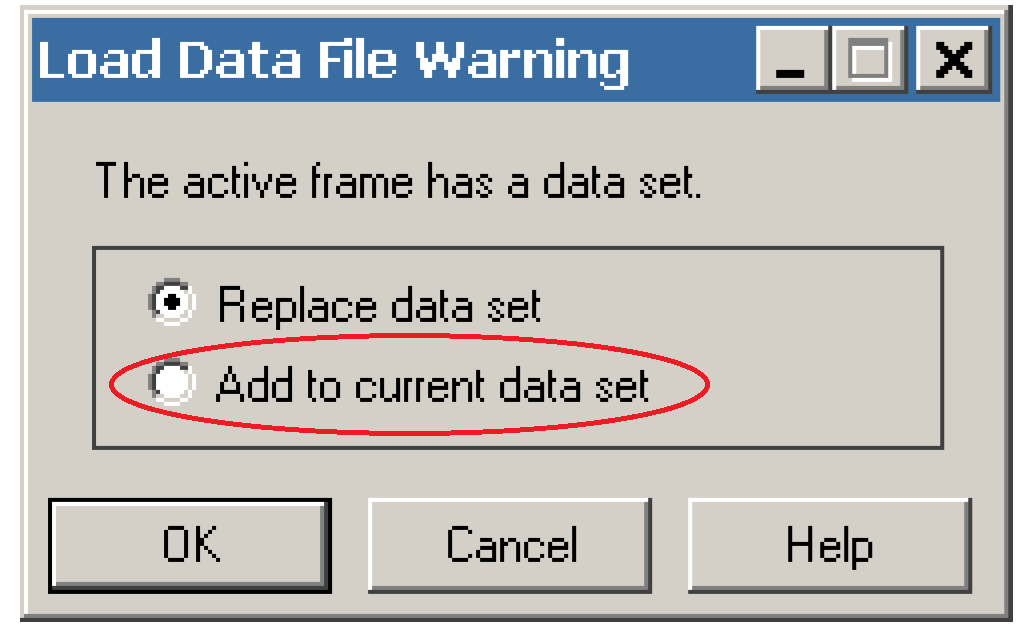
\includegraphics[width=0.6\textwidth]{./graphics/load_data}
%
\end{center}
\caption
[Load Data File Warning dialogue in TECPLOT]
{Load Data File Warning dialogue in TECPLOT.}
\label{fig:load_data}
\end{figure}

Once you have loaded your data with TECPLOT, the drogue positions will be
considered as ``Scatter plots'' by Tecplot Software. Scatter plots are plots of
symbols centered at the data points in a field. To add a scatter layer to your
plot, activate the ``Scatter'' toggle in the Sidebar. To be visible in your
plot, the Scatter layer which contains the Tecplot \telkey{ASCII DROGUES
FILE} must be turned on and the Scatter layer containing the \telkey{3D RESULT
FILE} data must be turned off. This is done by selecting ``Yes'' or ``No'' from
the [Scat Show] button drop-down menu on the Scatter page of the \textbf{Zone
Style dialogue} (cf. Figure \ref{fig:zone_style}).

\begin{figure}[H]%
\begin{center}
%
  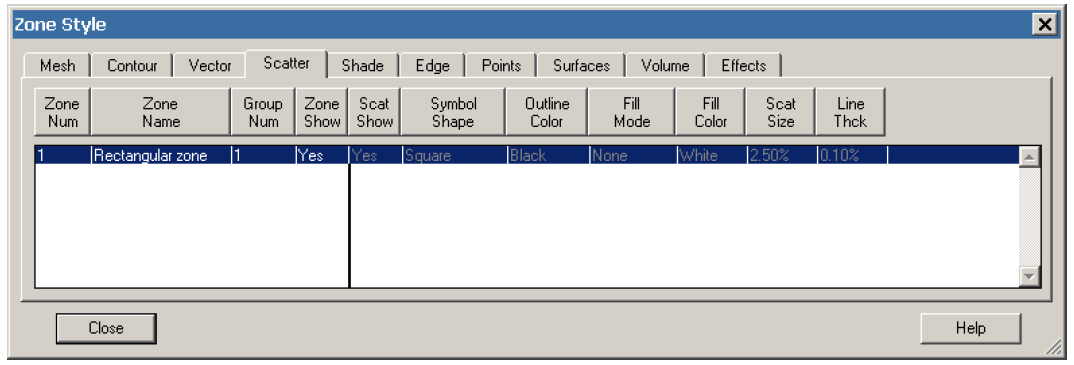
\includegraphics[width=0.7\textwidth]{./graphics/zone_style}
%
\end{center}
\caption
[Zone Style dialogue in TECPLOT]
{Zone Style dialogue in TECPLOT.}
\label{fig:zone_style}
\end{figure}

Then, you can modify your Scatter plot using the Scatter page of the
\textbf{Zone Style dialogue} and the Scatter submenu of the \textbf{Plot menu}.
You can control any of the following attributes for a zone or group of zones
from the Scatter page of the Zone Style dialogue. For complementary information
on the Tecplot procedure, the reader may refer to the Tecplot user guide.


%----------------------------------------------------------------------------------------
%	CHAPTER 9: Oil spill
%----------------------------------------------------------------------------------------

\chapter{Oil spill modelling}

During a hydrodynamic simulation, \telemac{3D} offers an opportunity to follow
the paths of an oil spill which is released into the fluid from a discharge
point.

The oil spill model introduced here combines an Eulerian and a Lagrangian
approach. The Lagrangian model simulates the transport of an oil spill near the
surface. The oil slick is represented by a large set of hydrocarbon particles.
Each particle is considered as a mixture of discrete non-interacting
hydrocarbon components. Particles are therefore represented by component
categories (soluble and unsoluble components), and the fate of each component
is tracked separately. Each particle has associated to it, amongst other
properties, an area, a mass, its barycentric coordinates within the element it
is located in, and the physico-chemical properties of each of its components.
The model accounts for the main processes that act on the spilled oil:
advection, effect of wind, diffusion, evaporation and dissolution. Though
generally considered to be a minor process, dissolution is important from the
point of view of toxicity. To simulate soluble oil component dissolution in
water, an Eulerian advection-diffusion model is used. The fraction of each
dissolved component is represented by a tracer whose mass directly depends on
the dissolved mass of oil particles. The hydrodynamic data required for either
Lagrangian and Eulerian transport approach are provided by the \telemac{3D}
hydrodynamic model. The oil spill theoretical background is explained in
\cite{JolyGoeury2013}.

The result of the oil spill modelling is provided in the form of a TECPLOT
formatted file which contains the various positions of the oil particles and a
\telemac{3D} result file (SERAFIN format) storing the oil dissolved components in
water column during the computation.


\section{Input files}

In addition to the minimum set of input files necessary to run a \telemac{3D}
case, an oil spill computation also needs an oil spill steering file.
Furthermore, to run an oil spill model the subroutine \telfile{OIL\_FLOT} needs
to be modified in the FORTRAN file.


\section{Steering file}

In addition to the necessary information for running the \telemac{3D}
hydrodynamic model the following essential information must be specified in the
\telemac{3D} steering file to run an oil spill propagation model:

\begin{itemize}
\item The use of the oil spill model must be declared: \telkey{OIL SPILL MODEL}
(= YES, default = NO),

\item The name of the oil spill steering file which contains the oil
characteristics: \telkey{OIL SPILL STEERING FILE} (\telkey{= name chosen by the
user}),

\item The number of oil releases during oil spill: \telkey{MAXIMUM NUMBER OF
DROGUES} (= number chosen by the user),

\item The frequency of the drogues printout period: \telkey{PRINTOUT PERIOD FOR
DROGUES} (= number chosen by the user),

\item The name of the tecplot oil file containing the oil displacement:
\telkey{ASCII DROGUES FILE} (= name chosen by the user, default = 1).
\end{itemize}

With the oil spill module, it is possible to take into account the transport of
soluble oil components in water (whose presence has no effect on the
hydrodynamics). These may or may not be diffused within the flow but their
characteristics have to be defined in the \telkey{OIL SPILL STEERING FILE}. If
these components are allowed to diffuse in the flow, they are then treated with
the tracer transport computations of \telemac{3D}. This implies that the
\telkey{NUMBER OF TRACERS} must be set to the number of the oil soluble
components. In addition the TRACER keywords, described in chapter 7, can be
specified.


\section{Oil spill steering file}

As seen previously, the \telkey{OIL SPILL STEERING FILE} name is given by the
user in the TELEMAC steering file. This file contains all the informations for
an oil spill calculations based on the composition considered by the user,
i.e.:

\begin{itemize}
\item The number of unsoluble components in oil,

\item The parameters of these components such as the mass fraction (\%) and
boiling point of each component (K),

\item The number of soluble components in oil,

\item The parameters of these components such as the mass fraction (\%),
boiling point of each component (K), solubility (kg.m${}^{-3}$) and the mass
transfer coefficient of the dissolution and volatilization phenomena
(m.s${}^{-1}$)

\item The oil density,

\item The oil viscosity (m${}^{2}$.s${}^{-1}$),

\item The volume of the spilled oil (m${}^{3}$),

\item The water surface temperature (K),

\item The spreading model chosen by the user:

\begin{itemize}
\item Fay's model,

\item Migr'Hycar model,

\item Constant area model.
\end{itemize}
\end{itemize}

\textbf{WARNING:}

\begin{WarningBlock}{Warning:}
\begin{itemize}
\item The parameters of soluble (or unsoluble) components need to be informed
only if the number of these components is not null

\item If the sum of all mass fraction components is not equal to 1, the run is
interrupted and the following error message is displayed:
\end{itemize}

\begin{lstlisting}[language=TelemacCas]
WARNING::THE SUM OF EACH COMPONENT MASS FRACTION IS NOT EQUAL TO 1.
PLEASE, MODIFY THE INPUT STEERING FILE
\end{lstlisting}
\end{WarningBlock}

An example of the oil spill steering file is given.

\begin{lstlisting}[language=bash]
NUMBER OF UNSOLUBLE COMPONENTS IN OIL
6
UNSOLUBLE COMPONENTS PARAMETERS (FRAC MASS, TEB)
5.1D-02       ,402.32D0
9.2D-02       ,428.37D0
3.16D-01      ,458.37D0
3.5156D-01    ,503.37D0
8.5D-02       ,543.37D0
9.4D-02       ,628.37D0
NUMBER OF SOLUBLE COMPONENTS IN OIL
4
SOLUBLE COMPONENTS PARAMETERS (FRAC MASS, TEB, SOL, KDISS, KVOL)
1.D-02   ,497.05D0,  0.018D0   , 1.25D-05 ,5.0D-05
3.2D-02  ,551.52D0,  0.00176D0 , 5.63D-06 ,1.51D-05
1.D-04   ,674.68D0,  2.0D-04   , 2.D-06   ,4.085D-07
2.D-05   ,728.15D0,  1.33D-06  , 1.33D-06 ,1.20D-07
OIL DENSITY
830.D0
OIL VISCOSITY
4.2D-06
OIL SPILL VOLUME
2.02D-05
WATER TEMPERATURE
292.05D0
SPREADING MODEL (1=FAY'S MODEL, 2=MIGR'HYCAR MODEL, 3=CONSTANT AREA)
2
\end{lstlisting}

If in the oil spill steering file, the SPREADING MODEL is set to 3, two lines
must be added to the previous example:

\begin{lstlisting}[language=bash]
CONSTANT AREA VALUE CHOSEN BY THE USER FOR EACH OIL PARTICLE
1 (example if the user wants area particle equal to 1 m2)
\end{lstlisting}


\section{The OIL\_FLOT subroutine}

After inserting the \telfile{OIL\_FLOT} subroutine in the FORTRAN file, it must
be modified it in order to indicate the release time step, together with the
coordinates of the release point. If the release point coordinates are outside
the domain, the run is interrupted and an error message is displayed. In
addition, if a particle leaves the domain during the simulation, it is of
course no longer monitored but its previous track remains in the results file
for consultation.

An example of modifications in the \telfile{OIL\_FLOT} subroutine is given.

The release time step in the first condition statement and the coordinates of
the release point must be changed:

\begin{lstlisting}[language=TelFortran]
...
IF(LT.EQ.10000)THEN
  NUM_GLO=0
  NUM_MAX=0
  NUM_LOC=0
  COORD_X=0.D0
  COORD_Y=0.D0
  NUM_MAX=INT(SQRT(REAL(NFLOT_MAX)))
  DO K=1,NUM_MAX
    DO J=1,NUM_MAX
      COORD_X=336000.D0+REAL(J)
      COORD_Y=371000.D0+REAL(K)
      NUM_GLO=NUM_GLO+1
      NFLOT_OIL=0
      CALL ADD_PARTICLEADD_PARTICLE(COORD_X,COORD_Y,0.D0,NUM_GLO,NFLOT_OIL,
&                       1,XFLOTXFLOT,YFLOTYFLOT,YFLOT,TAGFLOTAGFLO,
&                       SHPFLO,SHPFLO,ELTFLO,ELTFLO,MESH,1,
&                       0.D0,0.D0,0.D0,0.D0,0,0)
...
    END DO
  END DO
END IF
\end{lstlisting}


\section{Output files}

During an oil spill computation, the \telemac{3D} software produces at least two
output files:

\begin{itemize}
\item The \telkey{3D RESULT FILE},

\item The output \telkey{ASCII DROGUES FILE}.
\end{itemize}


\subsection{The 3d result file}

This is the file in which \telemac{3D} stores information during the computation.
It is normally in SERAFIN format. First of all, it contains information on the
mesh geometry, then the names of the stored variables. It then contains the
time for each time step and the values of the different variables for all mesh
points. For complementary information on the \telkey{3D RESULT FILE}, the
reader may refer to \ref{sec:3dres}.


\subsection{The output drogues file}

This is an ASCII file created by \telemac{3D} during the computation. It
stores drogue positions in TECPLOT format. To visualize the drogue positions
with Tecplot software, the user must:

\begin{itemize}
\item Use the File$>$Load Data File(s) command to load the \telkey{3D RESULT
FILE}

\item Use the File$>$Load Data File(s) command to load the Tecplot drogue file
\end{itemize}

See section \ref{sec:drogues} for more information as it is the same file as for drogues.



%----------------------------------------------------------------------------------------
%	CHAPTER 10: Other configurations
%----------------------------------------------------------------------------------------

\chapter{Others configurations}

\section{Modification of bottom topography (\telfile{CORFON})}

Bottom topography may be introduced at various levels, as stated in section
\ref{sec:topo}.

\telemac{3D} offers the possibility of modifying the bottom topography at the
beginning of a computation using the \telfile{T3D\_CORFON} subroutine. This is
called up once at the beginning of the computation and enables the value of
variable \telfile{ZF} to be modified at each point of the mesh. To do this, a number of
variables such as the point coordinates, the element surface value,
connectivity table, etc, are made available to the user.

By default, the \telfile{T3D\_CORFON} subroutine carries out a number of bottom
smoothings equal to \telfile{LISFON}, i.e. equal to the number specified by the keyword
\telkey{NUMBER OF BOTTOM SMOOTHINGS} for which the default value is 0 (no
smoothing).

The \telfile{T3D\_CORFON} subroutine is not called up if a computation is continued.
This avoids having to carry out several bottom smoothings or modifications to
the bottom topography during the computation.


\section{Modifying coordinates (\telfile{CORRXY})}

\telemac{3D} also offers the possibility of modifying the mesh point coordinates
at the beginning of a computation. This means, for example, that it is possible
to change the scale (from that of a reduced-scale model to that of the real
object), rotate or translate the object.

The modification is done in the \telfile{CORRXY} subroutine (\bief library), which
is called up at the beginning of the computation. This subroutine is empty by
default and gives an example of programming a change of scale and origin,
within commented statements.

It is also possible to specify the coordinates of the origin point of the mesh.
This is done using the keyword \telkey{ORIGIN COORDINATES} which specify 2
integers. These 2 integers will be transmitted to the results file in the
SERAFIN format, for a use by post-processors for superimposition of results
with digital maps (coordinates in meshes may be reduced to avoid dealing with
large real numbers). These 2 integers may also be used in subroutines under the
names \telfile{I\_ORIG} and \telfile{J\_ORIG}. Otherwise they do not have a use yet.


\section{Spherical coordinates (\telfile{LATITU})}

If a simulation is performed over a large domain, \telemac{3D} offers the
possibility of running the computation with spherical coordinates.

This option is activated when the keyword \telkey{SPHERICAL COORDINATES} is set
to YES (default value is NO). In this case, \telemac{3D} calls a subroutine named
\telfile{LATITU} through the subroutine \telfile{INBIEF} at the beginning of the
computation. This calculates a set of tables depending on the latitude of each
point. To do this, it uses the Cartesian coordinates of each point provided in
the geometry file, and the latitude of the point of origin of the mesh provided
by the user in the steering file with the keyword
\telkey{LATITUDE OF ORIGIN POINT}.

The spatial projection type used for the mesh is then specified with the
keyword \telkey{SPATIAL PROJECTION TYPE}. That can take the following values:
\begin{itemize}
\item 1 : Lambert Cartesian not geo referenced (default value -- cannot be used
in spherical)

\item 2 : Mercator;

\item 3 : Latitude/longitude (in degrees).
\end{itemize}

In this case of option 3, the coordinates of the mesh nodes should be
expressed with latitude and longitude in degrees. \telemac{3D} then converts with
the information with the help of the Mercator's projection.

The \telfile{LATITU} subroutine (\bief library) may be modified by the user to introduce
any other latitude-dependent computation.


\section{Adding new variables}
\label{sec:privarray}
A standard feature of \telemac{3D} is the storage of certain computed variables.
In certain cases, the user may wish to compute other variables and store them
in the results file (the number of variables is currently limited to four).

Since \telemac{3D} uses 2D and 3D variables, the treatments linked to these
variables may differ and call three subroutines:

\begin{itemize}
\item  \telfile{NOMVAR\_2D\_IN\_3D}: to manage 2D variables names,

\item  \telfile{NOMVAR\_TELEMAC3D}: to manage 3D variables names,

\item  \telfile{PRERES\_TELEMAC3D}: to compute new variables (2D and 3D).
\end{itemize}

\telemac{3D} has a numbering system in which, for example, the array containing
the Froude number has the number 7. The new variables created by the user may
have the numbers 25, 26, 27 and 28 (for 3D variables) and 27, 28, 29 and 30
(for 2D variables).

In the same way, each variable is identified by a letter in the keywords
\telkey{VARIABLES FOR 2D GRAPHIC PRINTOUTS} and
\telkey{VARIABLES FOR 3D GRAPHIC PRINTOUTS}.
The new variables are identified by the strings \telfile{PRIVE1, PRIVE2, PRIVE3}
and \telfile{PRIVE4} for 2D variables and \telfile{P1, P2, P3} and \telfile{P4}
for 3D variables.

At the end of the \telfile{NOMVAR\_XX} subroutine (XX = 2D or 3D), it is
possible to change the abbreviations (mnemonics) used for the keywords
\telkey{VARIABLES FOR GRAPHIC 2D PRINTOUTS} and \telkey{VARIABLES FOR GRAPHIC
3D}. Sequences of 8 letters may be used.
Consequently, the variables must be separated by spaces, commas or semi-colons
in the keywords, e.g.:

\begin{lstlisting}[language=TelemacCas]
VARIABLES FOR GRAPHIC PRINTOUTS : 'U, V, H, B'
\end{lstlisting}

In the software data structure, these four variables correspond to the tables
\telfile{PRIVE\%ADR(1)\%P\%R(X), PRIVE\%ADR(2)\%P\%R(X), PRIVE\%ADR(3)\%P\%R(X)}
and \telfile{PRIVE\%ADR(4)\%P\%R(X)} (in which \telfile{X} is the number of
nodes in the mesh). These may be used in several places in the programming,
like all TELEMAC variables.
For example, they may be used in the subroutines \telfile{CORRXY},
\telfile{CORSTR}, \telfile{BORD3D}, etc.  If a \telfile{PRIVE} table is used
to program a case, it is essential to check the value of the keyword
\telkey{NUMBER OF PRIVATE ARRAYS}.
This value fixes the number of tables used (0, 1, 2, 3 or 4)
and then determines the amount of memory space required. The user can also
access the tables via the aliases \telfile{PRIVE1, PRIVE2, PRIVE3} and
\telfile{PRIVE4}.

An example of programming using the second \telfile{PRIVE} table is given below.
It is initialised with the value 10.

\begin{lstlisting}[language=TelFortran]
DO I=1,NPOIN2
  PRIVE\%ADR(2)\%P\%R(I) = 10.D0
ENDDO
\end{lstlisting}

New variables are programmed in two stages:

\begin{itemize}
\item  Firstly, it is necessary to define the name of these new variables by
filling in the \telfile{NOMVAR\_TELEMAC3D} (or \telfile{NOMVAR\_2D\_IN\_3D})
subroutine. This consists of two equivalent structures, one for English and the
other for French. Each structure defines the name of the variables in the
results file that is to be generated and then the name of the variables to be
read from the previous computation if this is a restart. This subroutine
may also be modified when, for example, a file generated with the English
version of \telemac{3D} is to be continued with the French version. In this
case, the \telfile{TEXTPR} table of the French part of the subroutine must
contain the English names of the variables.

\item  Secondly, it is necessary to modify the \telfile{PRERES\_TELEMAC3D}
subroutine in order to introduce the computation of the new variable(s). The
variables \telfile{LEO, SORG2D} and \telfile{SORG3D} are also used to
determine whether the variable is to be printed in the printout file or in
the results file at the time step in question.
\end{itemize}

User arrays can be handled to store extra variables in 2D with the help of
two keywords to define the number and the name of the extra variables
in the 2D private arrays: \telkey{NUMBER OF 2D PRIVATE ARRAYS} (up to 4,
default value = 0) and \telkey{NAMES OF 2D PRIVATE VARIABLES}.
It is the names of the user arrays \telfile{PRIVE\%ADR(1)\%P, PRIVE\%ADR(2)\%P}
\ldots up to 4, that will be seen in the results files.
The great advantage is that these variables will be read if present in the
\telkey{GEOMETRY FILE}.

\section{Array modification or initialization}

When programming \telemac{3D} subroutines, it is sometimes necessary to
initialize a table or memory space to a particular value. To do that, the \bief
library furnishes a subroutine called \telfile{FILPOL} that lets the user modify or
initialize tables in particular mesh areas.

A call of the type \telfile{CALL FILPOL (F, C, XSOM, YSOM, NSOM, MESH)} fills
table \telfile{F} with the \telfile{C} value in the convex polygon defined by
\telfile{NSOM} nodes (coordinates \telfile{XSOM, YSOM}).
The variable \telfile{MESH} is needed for the \telfile{FILPOL} subroutine
but have no meaning for the user.


\section{Validating a computation (\telfile{VALIDA})}

The structure of the \telemac{3D} software offers an entry point for validating a
computation, in the form of a subroutine named \telfile{VALIDA}, which has to
be filled by the user in accordance with each particular case.
Validation may be carried out either with respect to a reference file (which is
therefore a file of results from the same computation that is taken as reference,
the name of which is supplied by the keyword \telkey{REFERENCE FILE}), or with
respect to an analytical solution that must then be programmed entirely by the user.

When using a reference file, the keyword \telkey{REFERENCE FILE FORMAT}
specifies the format of this binary file (SERAFIN by default).

The \telfile{VALIDA} subroutine is called at each time step when the keyword
\telkey{VALIDATION} has the value YES, enabling a comparison to be made with
the validation solution at each time step. By default, the \telfile{VALIDA}
subroutine only does a comparison with the last time step. The results of this
comparison are given in the output listing.


\section{Coupling}

The principle of coupling two (or in theory more) simulation modules involves
running the two calculations simultaneously and exchanging the various results
at each time step. For example, the following principle is used to couple a
hydrodynamic module and a sediment transport module:

\begin{itemize}
\item  The two codes perform the calculation at the initial instant with the
same information (in particular the mesh and bottom topography),

\item  The hydrodynamic code runs a time step and calculates the water depth
and velocity components. It provides this information to the sediment transport
code,

\item  The sediment transport code uses this information to run the solid
transport calculation over a time step and thus calculates a change in the
bottom,

\item  The new bottom value is then taken into account by the hydrodynamic
module at the next time step, and so on.
\end{itemize}

Two modules can be coupled in the current version of the code: the sedimentary
transport module SISYPHE and the sea state computational module \tomawac. The
time step used for the two calculations is not necessarily the same and is
managed automatically by the coupling algorithms and the keyword
\telkey{COUPLING PERIOD FOR SISYPHE} and \telkey{COUPLING PERIOD FOR TOMAWAC}
with default values 1 (coupling at every iteration).

This functionality requires two keywords. The keyword \telkey{COUPLING WITH}
indicates which simulation code is to be coupled with \telemac{3D}. The values of
this keyword can be:

\begin{itemize}
\item  \telkey{COUPLING WITH}= `SISYPHE' for coupling with the \sisyphe module,

\item  \telkey{COUPLING WITH}= `TOMAWAC' for coupling with the \tomawac module,

\item  \telkey{COUPLING WITH}= `SISYPHE, TOMAWAC' for coupling with both.
\end{itemize}

Depending on the module(s) used, the keywords \telkey{SISYPHE STEERING
FILE} and \telkey{TOMAWAC STEERING FILE} indicate the names of the steering files
of the coupled modules.

The keyword \telkey{COUPLING WITH} is also used if the computation has to
generate the appropriate files necessary to run a water quality simulation with
DELWAQ. In that case, it is necessary to specify \telkey{COUPLING WITH=
}'DELWAQ'. Please refer to Appendix \ref{sec:delwaq} for all informations
concerning communications with DELWAQ.

\section{Checking the mesh (\telfile{CHECKMESH})}

The subroutine \telfile{CHECKMESH} of the \bief library is available to look for
errors in the mesh, e.g. superimposed points \ldots
The keyword \telkey{CHECKING THE MESH} (default value = NO) should be activated
to YES to call this subroutine.

%----------------------------------------------------------------------------------------
%	CHAPTER 11: Parallelism
%----------------------------------------------------------------------------------------

\chapter{Parallelism}

For simulations requiring a high computational power, it can be advisable to
run the computations in multi-processor machines, or in clusters of
workstations. \telemac{3D} is available in a parallel version in order to take
advantage of that kind of computational architecture.

The \telemac{3D} parallel version uses the MPI library which has to be installed
beforehand to be implementable. The interface between \telemac{3D} and that MPI
library is achieved through the \telfile{parallel} library which is common to all
the TELEMAC system modules.

Lots of pieces of information concerning the implementation of the parallel
version can be found in the system's installation literature.

The user shall initially specify the number of processors used by means of the
keyword \telkey{PARALLEL PROCESSORS}. That integer type keyword can take the
following values:

\begin{itemize}
\item  0: Use of the conventional \telemac{3D} version (default),

\item  1: Use of the parallel \telemac{3D} version on one processor,

\item  2 ...: Use of the parallel \telemac{3D} version using the
specified number of processors.
\end{itemize}

Different partitioning tools may be used if installed.
They can be selected by the keyword \telkey{PARTITIONING TOOL} (default value
is METIS). The possible choices are:
\begin{itemize}
\item METIS,
\item SCOTCH,
\item PARMETIS,
\item PTSCOTCH \ldots
\end{itemize}


\appendix

%----------------------------------------------------------------------------------------
%	APPENDIX A: Launchin a simulation
%----------------------------------------------------------------------------------------

\chapter{Launching the computation}

A computation is launched through the \telfile{telemac3d.py} command.
That command activates the execution of a script which is common to all the
computation modules in the \tel system.
Depending on the platform, some options may be unavailable.

The syntaxes in that command are as follows:

\begin{lstlisting}[language=bash]
telemac3d.py [cas]   [--options]
\end{lstlisting}

\begin{itemize}
\item cas: name of the steering file,

\item --ncsize=NCSIZE: specifies the number of processors forced in parallel
mode, default = the number defined in the steering file,

\item -c CONFIGNAME or --configname=CONFIGNAME: specifies the configuration
name, default is randomly found in the configuration file,

\item -f CONFIGFILE, --configfile=CONFIGFILE: specifies the configuration
file, default = systel.cfg,

\item -s, --sortiefile: specifies whether there is a sortie file, default is
no,

\item -t or --tmpdirectory: the temporary work directory is not destroyed on
completion of computation.
\end{itemize}

By default, the procedure runs the computation in an interactive mode and
displays the control listing on the monitor.

The operations performed by that script are as follows:

\begin{itemize}
\item Creation of a temporary directory
(\telfile{name\_cas\_YYYY-MM-DD\_HHhMMminSSs}),

\item Duplication of the dictionary and the input files into that directory,

\item Execution of the \damo software in order to determine the work file names,

\item Creation of the computation launching script,

\item Allocation of the files,

\item Compilation of the FORTRAN file and link editing (as required),

\item Launching of the computation,

\item Retrieval of the results files and destruction of the temporary directory.
\end{itemize}

The procedure takes place with slight differences according to the selected
options.

The detailed description of that procedure can be obtained through the help
command:

\begin{lstlisting}[language=bash]
telemac3d.py --help
telemac3d.py -h
\end{lstlisting}



%----------------------------------------------------------------------------------------
%	APPENDIX B: List user subroutine
%----------------------------------------------------------------------------------------

\chapter{List of user subroutines}
\label{sec:usrsub}
Even though all subroutines can be modified by the user, some subroutines have
been specifically designed to define complex simulation parameters. They are
listed below:\\
\begin{tabular}{p{2.5in}p{4.0in}}
CALCOT       & Preparation of the array of mesh elevations between the bottom and the free surface\\
%CONDIN       &  Management of the initial conditions\\
CONDI3DH     &  Management of the initial conditions for water depth\\
CONDI3DTRAC  &  Management of the initial conditions for tracer(s)\\
CONDI3DUVW   &  Management of the initial conditions for velocity components\\
CONDIS       &  Initialization of the arrays of the physical sedimentological quantities\\
CORRXY       & Modification of the mesh node co-ordinates\\
CORSTR       & Correction of the bottom friction coefficient when it is time-variable\\
DECLARATIONS\_TELEMAC3D & Statement of the \telemac{3D} structures\\
DRIUTI       &  User damping function\\
DRSURR       &  Computation of density (equation of state)\\
FLOT3D       &  Initial conditions of the drogues\\
LIMI3D       &  Management of the boundary conditions\\
MESH\_TRANSF &  Definition of the mesh transformation (distribution of the horizontal planes)\\
NOMVAR\_TELEMAC3D & Management of the names of variables for the graphic printouts\\
PRERES\_TELEMAC3D & Computation of the output variables (free surface, flow rate\dots )\\
Q3     &  Management of the flow rates in a boundary condition\\
%SCOPE  &  Creation of 1D sections\\
SL3    &  Management of the open surface in a boundary condition\\
SOURCE &  User source term in the hydrodynamic equation\\
SOURCE\_TRAC & User source term in the equations of tracers\\
T3D\_CORFON  &  Modification of bottoms\\
TR3    & Management of the tracers in a boundary condition\\
TRISOU &  Source terms for the velocity components\\
USER\_BORD3D &  Management of the boundary conditions\\
UTIMP  &  Additional variable writing\\
VEL\_PROF\_Z & Definition of the vertical velocity profile\\
VISCLM  & Computation of the viscosity in the mixing length models\\
VISCOS  &  Computation and initialization of the constant viscosity\\
VIT3    &  Management of the velocities in a boundary condition\\
\end{tabular}


%----------------------------------------------------------------------------------------
%	APPENDIX C: Serafin format
%----------------------------------------------------------------------------------------

\chapter{The SELAFIN format}\label{sec:srffmt}

Note: for unclear historical reasons this format is also sometimes called SERAFIN

This is a binary file.

This format can be `SERAFIN `, for single precision storage, or `SERAFIND' for
double precision storage.  Double precision storage can be used for cleaner
restarts, but may not be understood by all post-processors.

All string in the SERAFIN file must be utf-8 encoded (See for
\url{https://en.wikipedia.org/wiki/UTF-8} for the exact list).

The records are listed below. Records are given in the FORTRAN sense. It means
that every record corresponds to a FORTRAN WRITE:

1 record containing the title of the study (80 characters), The last 8
characters must contain the format of the file (SERAFIN or SERAFIND)

1 record containing the two integers NBV(1) and
NBV(2) (NBV(1) the number of variables, NBV(2)
with the value of 0),

NBV(1) records containing the names and units of each variable (over 32
characters),

1 record containing the integers table IPARAM (10 integers, of which only 4 are
currently being used).

If IPARAM (3) is not 0: the value corresponds to the x-coordinate of the origin
in the mesh

If IPARAM (4) is not 0: the value corresponds to the y-coordinate of the origin
in the mesh

These coordinates in metres may be used by post-processors to retrieve
geo-referenced coordinates, while the coordinates of the mesh are relative to
keep more digits.

If IPARAM (7) is not 0: the value corresponds to the number of planes on the
vertical (in prisms.)

If IPARAM (8) is not 0: the value corresponds to the number of boundary points
(in parallel).

If IPARAM (9) is not 0: the value corresponds to the number of interface points
(in parallel).

if IPARAM (10) = 1: a record containing the computation starting date in 6
integers: year, month, day, hour, minute, second

1 record containing the integers NELEM,NPOIN,NDP,1 (number of elements, number
of points, number of points per element and the value 1),

1 record containing table IKLE (integer array of dimension (NDP,NELEM) which is
the connectivity table. Beware: in \telemac{2D}, the dimensions of this array
are (NELEM,NDP)),

1 record containing table IPOBO (integer array of dimension NPOIN); the value
is 0 for an internal point, and gives the numbering of boundary points for the
others. This array is never used (its data can be retrieved by another way). In
parallel the table KNOLG is given instead, keeping track of the global numbers
of points in the original mesh.

1 record containing table X (real array of dimension NPOIN containing the
abscissas of the points),

1 record containing table Y (real array of dimension NPOIN containing the
ordinates of the points),

Next, for each time step, the following are found:
\begin{itemize}
  \item 1 record containing time T (real),
  \item NBV(1)+NBV(2) records containing the results arrays for each variable
    at time T.
\end{itemize}



%----------------------------------------------------------------------------------------
%	APPENDIX D: Delwaq
%----------------------------------------------------------------------------------------

\chapter{Generating output files for DELWAQ}
\label{sec:delwaq}
The \telemac{3d} software is able to generate the appropriate files necessary to
run a DELWAQ water quality simulation. This generation is managed only
through the following keywords:

\begin{tabular}{l}
\telkey{BOTTOM SURFACES DELWAQ FILE}\\
\telkey{DELWAQ PRINTOUT PERIOD}\\
\telkey{DELWAQ STEERING FILE}\\
\telkey{DIFFUSION FOR DELWAQ}\\
\telkey{DIFFUSIVITY DELWAQ FILE}\\
\telkey{EXCHANGE AREAS DELWAQ FILE}\\
\telkey{EXCHANGES BETWEEN NODES DELWAQ FILE}\\
\telkey{NODES DISTANCES DELWAQ FILE}\\
\telkey{SALINITY DELWAQ FILE}\\
\telkey{SALINITY FOR DELWAQ}\\
\telkey{TEMPERATURE DELWAQ FILE}\\
\telkey{TEMPERATURE FOR DELWAQ}\\
\telkey{VELOCITY DELWAQ FILE}\\
\telkey{VELOCITY FOR DELWAQ}\\
\telkey{VERTICAL FLUXES DELWAQ FILE}\\
\telkey{VOLUMES DELWAQ FILE}\\
\end{tabular}

More information about these keywords can be found in the \telemac{3d} reference
manual. For more information, please refer to the DELWAQ user documentation.


%----------------------------------------------------------------------------------------
%	APPENDIX E: some recommendations
%----------------------------------------------------------------------------------------

\chapter{Some recommendations for TELEMAC-3D simulations}

If it is not too bad for you to increase your computational time,
here are some recommendations about the options to use.

\section{Advection}
\begin{itemize}
\item use the predictor-corrector distributive scheme with local implicitation for tidal flats,
based on the PSI scheme, for the velocity and all tracers, including $k$ and $\epsilon$
if you have them:\\
  / PSI scheme\\
  \telkey{SCHEME FOR ADVECTION OF VELOCITIES} = 5\\
  \telkey{SCHEME FOR ADVECTION OF K-EPSILON} = 5\\
  \telkey{SCHEME FOR ADVECTION OF TRACERS} = 5\\
  / predictor-corrector with local implicitation implicite\\
  \telkey{SCHEME OPTION FOR ADVECTION OF VELOCITIES} = 4\\
  \telkey{SCHEME OPTION FOR ADVECTION OF K-EPSILON} = 4\\
  \telkey{SCHEME OPTION FOR ADVECTION OF TRACERS} = 4\\
These are the new default values since version 8.1.\\
\item without tidal flats, use the predictor-corrector without tidal flats treatment to gain some time\\
  / Predictor-corrector without tidal flats treatment\\
  \telkey{SCHEME OPTION FOR ADVECTION OF VELOCITIES} = 2\\
  \telkey{SCHEME OPTION FOR ADVECTION OF K-EPSILON} = 2\\
  \telkey{SCHEME OPTION FOR ADVECTION OF TRACERS} = 2\\
\end{itemize}
\section{Friction}
\begin{itemize}
\item use the Nikuradse law, which is the only one that is really 3D compatible:
the other options have been implemented to ensure an easy correspondance between 2D and 3D simulations,
but their use is not recommended for fully 3D studies:\\
  \telkey{LAW OF BOTTOM FRICTION} = 5,\\
\item use a friction coefficient that is representative of the physics of your case:
with the Nikuradse law, the friction coefficient corresponds to the characteristic height of the roughness \\
  \telkey{FRICTION COEFFICIENT FOR THE BOTTOM} = 3 $\times$ d90.\\
  For a natural bed with sediment of characteristic size d90 and without riddles or dunes,
its value should be taken from van Rijn, equal to 3 $\times$ d90.
In the presence of dunes, van Rijn proposes another formula,
\item depending on the nature of the lateral walls, either use a Nikuradse law or no friction \\
  \telkey{LAW OF FRICTION ON LATERAL BOUNDARIES} = 0 or 5,
\item as for the bed, use a physical value for \telkey{FRICTION COEFFICIENT FOR LATERAL SOLID BOUNDARIES},
\item remark: contrary to the friction coefficients used with the laws derived
from the shallow water context (Manning, Strickler, Chézy, Haaland),
the friction coefficient with the Nikuradse law does not "hide" physical effects
like diffusion-dispersion, like it does with the shallow-water equations.
Thus, it is less prone to being used as a calibration parameter in the studies.
\end{itemize}

\section{Mass-lumping}
\begin{itemize}
\item avoid using mass-lumping, unless you really have a strong constraint on computational time
(this is the default behaviour of TELEMAC-3D): it introduces artificial dispersion in the results.
\end{itemize}

\section{Semi-implicitation}
\begin{itemize}
\item do not change the default value for\\
  \telkey{IMPLICITATION FOR DEPTH} ( = 0.55)\\
  and use \\
  \telkey{IMPLICITATION FOR VELOCITIES} = 0.55, new default value since version 8.1. \\
%instead of the default value of 1.
Warning: never use a value lower or equal to 0.5 for these coefficients,
otherwise the scheme becomes unconditionnally unstable. Avoid using the value 1 too, we have observed a
strange behaviour of the scheme in this case: it seems to introduce quite a lot of spurious diffusion,
even though 0.99 does not... We should perform more testing and analysis to better understand this behaviour.
\item the keyword \telkey{IMPLICITATION FOR DIFFUSION} can be left to its value by default, 1.
\end{itemize}

\section{Linear solvers}
\begin{itemize}
\item use the GMRES solver (= 7) for the matrices inversion, except diffusion
(\telkey{SOLVER FOR PPE, SOLVER FOR PROPAGATION}).
For the diffusion, the conjugate gradients should be good enough (solver number = 1).
These are the new default values since version 8.1,
\item use an accuracy equal to $10^{-8}$ or lower for all solvers
(\telkey{ACCURACY FOR PPE, ACCURACY FOR PROPAGATION, ACCURACY FOR DIFFUSION OF VELOCITIES,
ACCURACY FOR DIFFUSION OF K-EPSILON, ACCURACY FOR DIFFUSION OF TRACERS, ACCURACY FOR DIFFUSION OF SEDIMENT}).
These are the new default values since version 8.1,
\item be careful to always check in your listing that your solvers have actually converged,
otherwise the simulation may complete but with wrong results.
In case you do not reach the accuracy you asked for with these options,
try increasing the value of \telkey{OPTION OF SOLVER FOR [...]} to 10.
It sets the size of the Krylov subspaces used in the GMRES solver.
You can also try using conjugate gradients or Bi-CGSTAB,
or increasing the maximum number of iterations of the solvers,
or try using the preconditionning number 34 to make the matrix inversions faster.
\end{itemize}

\section{Fractional steps method}
\begin{itemize}
\item the keyword \telkey{DYNAMIC PRESSURE IN WAVE EQUATION} can be left to its value by default NO,
but setting it to YES may slightly reduce the numerical diffusion
(altough we need to test it further to really characterize the behaviour of these two choices).
\end{itemize}

\section{Free surface}
\begin{itemize}
\item if you observe free-surface instabilities (wiggles) in your results,
you can try using a lower value for the\\
\telkey{FREE SURFACE GRADIENT COMPATIBILITY}\\
than the one by default, for example 0.9.
\end{itemize}

\section{Liquid boundaries}
\begin{itemize}
\item we would suggest trying not to use the Thompson boundary conditions,
because they are actually only valid in the shallow water context.
However, they may help stabilise the simulations involving liquid boundaries,
so it is not always that easy not to use them.
You should try without it before trying to use it.
\end{itemize}

\section{Tidal flats}
\begin{itemize}
\item use \telkey{TREATMENT OF NEGATIVE DEPTHS} = 2 if possible,
\item use \telkey{TREATMENT ON TIDAL FLATS FOR TRACERS} = 1 to ensure conservation.
\end{itemize}

\section{Turbulence}
\begin{itemize}
\item trying to use the $k$-$\epsilon$ model (= 3) on the vertical and the horizontal directions,
or the Spalart-Allmaras one (= 5), also in both directions,
instead of the mixing length model which is not flexible, since it is a zero-equation model.
However, for stratification simulations, the mixing length model
may provide better results than any other (the $k-\epsilon$ model tends to mix too much).
\end{itemize}

\section{Other numerical options}
\begin{itemize}
\item do not change the matrix storage, simply do not include it from the steering file.
\end{itemize}



%---------------------------------------------------------------------------
% Bibliography
%---------------------------------------------------------------------------
\bibliographystyle{plainnat}
\bibliography{../../data/biblio}
\addcontentsline{toc}{chapter}{Bibliography}

\end{document}
